%% 使用 njuthesis 文档类生成南京大学学位论文的示例文档
%%
%% 作者:胡海星,starfish (at) gmail (dot) com
%% 项目主页: http://haixing-hu.github.io/nju-thesis/
%%
%% 本样例文档中用到了吕琦同学的博士论文的提高和部分内容,在此对他表示感谢。
%%
\documentclass[phd, macfonts]{njuthesis}
%% njuthesis 文档类的可选参数有:
%%   nobackinfo 取消封二页导师签名信息。注意,按照南大的规定,是需要签名页的。
%%   phd/master/bachelor 选择博士/硕士/学士论文

% 使用 blindtext 宏包自动生成章节文字
% 这仅仅是用于生成样例文档,正式论文中一般用不到该宏包
% \usepackage[math]{blindtext}
\usepackage{graphicx, caption, url, footnote, afterpage, epigraph}
\usepackage{tabularx, multicol, amssymb, bm, amsmath}
%\usepackage{tocbibind, tocloft, xpatch}
\usepackage[figuresright]{rotating}
\usepackage[list=true,listformat=simple]{subcaption}
\newcommand{\tif}{\mathrm}
\renewcommand{\labelenumi}{\roman{enumi}.}
\newcommand{\vect}[1]{\boldsymbol{#1}}
\renewcommand\labelenumi{\theenumi.}
\newcommand*{\citen}{}% generate error, if `\citen` is already in use
\DeclareRobustCommand*{\citen}[1]{%
  \begingroup
    \romannumeral-`\x % remove space at the beginning of \setcitestyle
    \setcitestyle{numbers}%
    \cite{#1}%
  \endgroup
}
\newcommand{\RN}[1]{%
  \textup{\uppercase\expandafter{\romannumeral#1}}%
}
\newcommand*\cleartoleftpage{%
  \clearpage
  \ifodd\value{page}\hbox{}\newpage\fi
}
%%%%%%%%%%%%%%%%%%%%%%%%%%%%%%%%%%%%%%%%%%%%%%%%%%%%%%%%%%%%%%%%%%%%%%%%%%%%%%%
% 设置《国家图书馆封面》的内容,仅博士论文才需要填写

% 设置论文按照《中国图书资料分类法》的分类编号
\classification{0175.2}
% 论文的密级。需按照GB/T 7156-2003标准进行设置。预定义的值包括:
% - \openlevel,表示公开级:此级别的文献可在国内外发行和交换。
% - \controllevel,表示限制级:此级别的文献内容不涉及国家秘密,但在一定时间内
%   限制其交流和使用范围。
% - \confidentiallevel,表示秘密级:此级别的文献内容涉及一般国家秘密。
% - \clasifiedlevel,表示机密级:此级别的文献内容涉及重要的国家秘密 。
% - \mostconfidentiallevel,表示绝密级:此级别的文献内容涉及最重要的国家秘密。
% 此属性可选,默认为\openlevel,即公开级。
\securitylevel{\openlevel}
% 设置论文按照《国际十进分类法UDC》的分类编号
% 该编号可在下述网址查询:http://www.udcc.org/udcsummary/php/index.php?lang=chi
\udc{004.72}
% 国家图书馆封面上的论文标题第一行,不可换行。此属性可选,默认值为通过\title设置的标题。
\nlctitlea{巡天时域光变序列分析与}
% 国家图书馆封面上的论文标题第二行,不可换行。此属性可选,默认值为空白。
\nlctitleb{太阳系外热类木星统计}
% 国家图书馆封面上的论文标题第三行,不可换行。此属性可选,默认值为空白。
\nlctitlec{}
% 导师的单位名称及地址
\supervisorinfo{南京大学天文与空间科学学院~~南京市仙林大道~163~号~~210089}
% 答辩委员会主席
\chairman{A~~教授}
% 第一位评阅人
\reviewera{B~~教授}
% 第二位评阅人
\reviewerb{C~~副教授}
% 第三位评阅人
\reviewerc{D~~教授}
% 第四位评阅人
\reviewerd{E~~研究员}

%%%%%%%%%%%%%%%%%%%%%%%%%%%%%%%%%%%%%%%%%%%%%%%%%%%%%%%%%%%%%%%%%%%%%%%%%%%%%%%
% 设置论文的中文封面

% 论文标题,不可换行
%\title{}
% 如果论文标题过长,可以分两行,第一行用\titlea{}定义,第二行用\titleb{}定义,将上面的\title{}注释掉
\titlea{巡天时域光变序列分析与}
\titleb{太阳系外热类木星统计}
% 论文作者姓名
\author{孟泽洋}
% 论文作者联系电话
\telphone{15950459632}
% 论文作者电子邮件地址
\email{mengzy1989@gmail.com}
% 论文作者学生证号
\studentnum{DG1326007}
% 论文作者入学年份(年级)
\grade{2013}
% 导师姓名职称
\supervisor{周济林~~教授}
% 导师的联系电话
\supervisortelphone{13512540416}
\cosupervisor{林潮~~教授}
% 论文作者的学科与专业方向
\major{天文学}
% 论文作者的研究方向
\researchfield{太阳系外行星的探测与统计}
% 论文作者所在院系的中文名称
\department{天文与空间科学学院}
% 论文作者所在学校或机构的名称。此属性可选,默认值为``南京大学''。
\institute{南京大学}
% 论文的提交日期,需设置年、月、日。
\submitdate{2017年5月10日}
% 论文的答辩日期,需设置年、月、日。
\defenddate{2017年6月1日}
% 论文的定稿日期,需设置年、月、日。此属性可选,默认值为最后一次编译时的日期,精确到日。
%% \date{2013年5月1日}
%%%%%%%%%%%%%%%%%%%%%%%%%%%%%%%%%%%%%%%%%%%%%%%%%%%%%%%%%%%%%%%%%%%%%%%%%%%%%%%
% 设置论文的英文封面

% 论文的英文标题,不可换行
\englishtitle{Light Curve Analysis of Optical Surveys and Statistics of Hot Jupiters}
% 论文作者姓名的拼音
\englishauthor{Meng Ze-Yang}
% 导师姓名职称的英文
\englishsupervisor{Professor Zhou Ji-Lin (NJU)}
\englishcosupervisor{Professor Douglas Lin (UCSC) \& Alice Quillen (UofR)}
% 论文作者学科与专业的英文名
\englishmajor{Astronomy}
% 论文作者所在院系的英文名称
\englishdepartment{Department of Astronomy and Space Science}
% 论文作者所在学校或机构的英文名称。此属性可选,默认值为``Nanjing University''。
\englishinstitute{Nanjing University}
% 论文完成日期的英文形式,它将出现在英文封面下方。需设置年、月、日。日期格式使用美国的日期
% 格式,即``Month day, year'',其中``Month''为月份的英文名全称,首字母大写;``day''为
% 该月中日期的阿拉伯数字表示;``year''为年份的四位阿拉伯数字表示。此属性可选,默认值为最后
% 一次编译时的日期。
\englishdate{May 1, 2017}
%%%%%%%%%%%%%%%%%%%%%%%%%%%%%%%%%%%%%%%%%%%%%%%%%%%%%%%%%%%%%%%%%%%%%%%%%%%%%%%
% 设置论文的中文摘要
% 设置中文摘要页面的论文标题及副标题的第一行。
% 此属性可选,其默认值为使用|\title|命令所设置的论文标题
\abstracttitlea{巡天时域光变序列分析与}
% 设置中文摘要页面的论文标题及副标题的第二行。
% 此属性可选,其默认值为空白
\abstracttitleb{太阳系外热类木星统计}
%%%%%%%%%%%%%%%%%%%%%%%%%%%%%%%%%%%%%%%%%%%%%%%%%%%%%%%%%%%%%%%%%%%%%%%%%%%%%%%
% 设置论文的英文摘要
% 设置英文摘要页面的论文标题及副标题的第一行。
% 此属性可选,其默认值为使用|\englishtitle|命令所设置的论文标题
\englishabstracttitlea{Light Curve Analysis of Optical Surveys and}
% 设置英文摘要页面的论文标题及副标题的第二行。
% 此属性可选,其默认值为空白
\englishabstracttitleb{Statistics of Hot Jupiters} 
%%%%%%%%%%%%%%%%%%%%%%%%%%%%%%%%%%%%%%%%%%%%%%%%%%%%%%%%%%%%%%%%%%%%%%%%%%%%%%%
\begin{document}
%%%%%%%%%%%%%%%%%%%%%%%%%%%%%%%%%%%%%%%%%%%%%%%%%%%%%%%%%%%%%%%%%%%%%%%%%%%%%%%

% 制作国家图书馆封面(博士学位论文才需要)
\makenlctitle
% 制作中文封面
\maketitle
% 制作英文封面
\makeenglishtitle


%%%%%%%%%%%%%%%%%%%%%%%%%%%%%%%%%%%%%%%%%%%%%%%%%%%%%%%%%%%%%%%%%%%%%%%%%%%%%%%
% 开始前言部分
\frontmatter
%%%%%%%%%%%%%%%%%%%%%%%%%%%%%%%%%%%%%%%%%%%%%%%%%%%%%%%%%%%%%%%%%%%%%%%%%%%%%%%
% 论文的中文摘要
%%%%%%%%%%%%%%%%%%%%%%%%%%%%%%%%%%%%%%%%%%%%%%%%%%%%%%%%%%%%%%%%%%%%%%%%%%%%%%%
%%  
%% 文档类 NJU-Thesis 用户手册
%%
%% 作者:胡海星,starfish (at) gmail (dot) com
%% 项目主页: https://github.com/Haixing-Hu/nju-thesis
%%
%% This file may be distributed and/or modified under the conditions of the
%% LaTeX Project Public License, either version 1.2 of this license or (at your
%% option) any later version. The latest version of this license is in:
%%
%% http://www.latex-project.org/lppl.txt
%%
%% and version 1.2 or later is part of all distributions of LaTeX version
%% 1999/12/01 or later.
%%
%%%%%%%%%%%%%%%%%%%%%%%%%%%%%%%%%%%%%%%%%%%%%%%%%%%%%%%%%%%%%%%%%%%%%%%%%%%%%%%


% 设置论文的中文摘要
% 设置中文摘要页面的论文标题及副标题的第一行。
% 此属性可选,其默认值为使用|\title|命令所设置的论文标题
%% \abstracttitlea{}
% 设置中文摘要页面的论文标题及副标题的第二行。
% 此属性可选,其默认值为空白
%% \abstracttitleb{}

% 论文的中文摘要

\begin{abstract}
% 中文关键词。关键词之间用中文全角分号隔开,末尾无标点符号。
\keywords{}
\end{abstract}
%%%%%%%%%%%%%%%%%%%%%%%%%%%%%%%%%%%%%%%%%%%%%%%%%%%%%%%%%%%%%%%%%%%%%%%%%%%%%%%
% 论文的英文摘要
%%%%%%%%%%%%%%%%%%%%%%%%%%%%%%%%%%%%%%%%%%%%%%%%%%%%%%%%%%%%%%%%%%%%%%%%%%%%%%%
%%  
%% 文档类 NJU-Thesis 用户手册
%%
%% 作者:胡海星,starfish (at) gmail (dot) com
%% 项目主页: https://github.com/Haixing-Hu/nju-thesis
%%
%% This file may be distributed and/or modified under the conditions of the
%% LaTeX Project Public License, either version 1.2 of this license or (at your
%% option) any later version. The latest version of this license is in:
%%
%% http://www.latex-project.org/lppl.txt
%%
%% and version 1.2 or later is part of all distributions of LaTeX version
%% 1999/12/01 or later.
%%
%%%%%%%%%%%%%%%%%%%%%%%%%%%%%%%%%%%%%%%%%%%%%%%%%%%%%%%%%%%%%%%%%%%%%%%%%%%%%%%


% 设置论文的英文摘要
% 设置英文摘要页面的论文标题及副标题的第一行。
% 此属性可选,其默认值为使用|\englishtitle|命令所设置的论文标题
%% \englishabstracttitlea{}
% 设置英文摘要页面的论文标题及副标题的第二行。
% 此属性可选,其默认值为空白
%% \englishabstracttitleb{}
% 论文的英文摘要


\begin{englishabstract}

% 英文关键词。关键词之间用英文半角逗号隔开,末尾无符号。
\englishkeywords{}
\end{englishabstract}
%%%%%%%%%%%%%%%%%%%%%%%%%%%%%%%%%%%%%%%%%%%%%%%%%%%%%%%%%%%%%%%%%%%%%%%%%%%%%%%
% 论文的前言,应放在目录之前,中英文摘要之后
%% Zeyang Meng PhD Thesis 2017.
%%
\begin{preface} 

\epigraph{... Der bestirnte Himmel über mir, und das moralische Gesetz in mir.}{\textit{Immanuel Kants}}

\vspace{1cm}

自诞生以来,人类就从未停止向外界探索以及反思自我。从技术层面上看,在望远镜
分辨率与灵敏度被推向极限的同时,科学家们也在考究着生命与宜居行星存在的合理
性。现如今太阳系外行星(简称:系外行星)科学领域,与传统的行星科学相比,虽
然诞生并未满半个世纪,但也正尝试以「它山之石」 -- 其它恒星周围的行星们,来内
窥太阳系行星系统以及生命本身。
\\ \par
近二十年来,随着观测技术的迭代更新,被探测到的系外行星样本也在正加速地扩大,
以往得到的基于太阳系行星系统的传统行星形成理论也随之不停地被改进、更正。正
当行星的形成阶段一次次地被观测到(如行星形成早期的原行星盘),一些看似与太
阳系大不同的系外行星系统(如周期小于十天的热木星)也不断地完善并细化着已知
的行星系统动力学作用理论。系外行星领域也正随之如此恰似涓涓细流般启发着人类
对太阳系起源与系外生命的认知。
\\ \par
而以上这一切里程碑,正离不开高精度数据预处理与前卫的理论分析和计算,如基于
地面的高精度光谱仪 HIRES 和 $Kepler$ 太空望远镜等仪器的数据处理流程。此册博
士论文也借此尝试从高精度数据处理入手(「中国之星」 中的「鬼像」处理),去探
寻可能的系外原始行星盘(搜索大麦哲伦云星系中的掩食盘候选体),并且从统计上
对现有的热木星系统的形成与潮汐演化作出部分限制(平衡潮汐模型下,热木星轨道
法向与宿主恒星自转轴取向不一致性在统计上的物理性质)。
\\ \par
作为一门跨学科领域,如今系外行星也正通往着融合了天体生物和行星大气等多科学
的方向发展。Spitzer 太空望远镜也已观测到数十颗系外行星大气存在的证据。在不久
的将来,光合化学与有机分子化学也会被有效地应用到如何将观测到的光信号转化成
生命存在的证据。科学家们也正在摸索中走出一条通往太阳系的起源与太阳系外生命
之路,而此刻的人类是否已蓄势待发准备好迎接新的纪元...


\vfill

\hfill 孟泽洋

\hfill 丁酉年正月廿七

\hfill 南京大学

\end{preface}

%%%%%%%%%%%%%%%%%%%%%%%%%%%%%%%%%%%%%%%%%%%%%%%%%%%%%%%%%%%%%%%%%%%%%%%%%%%%%%%
% 生成论文目次
\tableofcontents
%%%%%%%%%%%%%%%%%%%%%%%%%%%%%%%%%%%%%%%%%%%%%%%%%%%%%%%%%%%%%%%%%%%%%%%%%%%%%%%
% 生成插图清单。如无需插图清单则可注释掉下述语句。
\listoffigures
%%%%%%%%%%%%%%%%%%%%%%%%%%%%%%%%%%%%%%%%%%%%%%%%%%%%%%%%%%%%%%%%%%%%%%%%%%%%%%%
% 生成附表清单。如无需附表清单则可注释掉下述语句。
\listoftables
%%%%%%%%%%%%%%%%%%%%%%%%%%%%%%%%%%%%%%%%%%%%%%%%%%%%%%%%%%%%%%%%%%%%%%%%%%%%%%%

%\listofequations   ????????????????????????????

% 开始正文部分
\mainmatter
%%%%%%%%%%%%%%%%%%%%%%%%%%%%%%%%%%%%%%%%%%%%%%%%%%%%%%%%%%%%%%%%%%%%%%%%%%%%%%%
% 学位论文的正文应以《绪论》作为第一章
\chapter{绪论} \label{chapter:intro}

%\epigraph{... the ways by which men arrive at knowledge of the celestial things are hardly less wonderful than the nature of these things themselves}{\textit{Johannes Kepler}}

\section{引言}
\subsection{地球与人类,无独有偶?}

由古至今,人类在宇宙中的所处的位置就一直魂牵梦绕着人们的思绪。这个难题既
包括了人类居住的地球在空间上究竟是否独特,另一方面也包含人类(或生命)在宇
宙中的唯一性与否。而正因人类拥有了实证与思考的能力,因而在这个问题上的观测
与探索也从未曾停歇。

首先,行星科学(Planetology)是一门古老的以观测为基础的科学。早在公元前,古
希腊等各大文明已有天文学家(如伊巴谷)统计了相当可观的夜空发光天体的运行与
方位\cite{Xuan1992, wikipedia_astronomer}。而在以托勒密为代表所提倡的
地心说主导了这个星球一千多年后,文艺复兴时期的哥白尼等人也通过观测提出了日
心说\cite{Copernicus1543}。自此地球在空间位置谜团便开始层层被揭开,
地球的面貌(图 \ref{fig:rwalone})也愈发完整地展现在了人类面前。

\afterpage{
\begin{savenotes}
\begin{figure}[ht]
\centering
\begin{subfigure}[b]{.45\textwidth}
\captionsetup{width=0.9\textwidth}
\centering
\includegraphics[width=0.95\textwidth]{figures/chapter1/fig1a_Apollo17_BlueMarble.jpg}
\caption[Apollo 17 号船员拍摄的南半地球,拍摄时间 1972 年 12 月 7 日。(图片版权:NASA)]{Apollo 17 号船员拍摄的南半地球\footnotemark[1],拍摄日期为 1972 年 12 月 7 日。(图片版权:NASA)}
\label{fig:apollo17earth}
\setcounter{footnote}{1}
\addtocounter{footnote}{+0}\footnotetext{\url{https://www.nasa.gov/content/blue-marble-image-of-the-earth-from-apollo-17}}
\end{subfigure}
\begin{subfigure}[b]{.45\textwidth}
\captionsetup{width=0.9\textwidth}
\centering
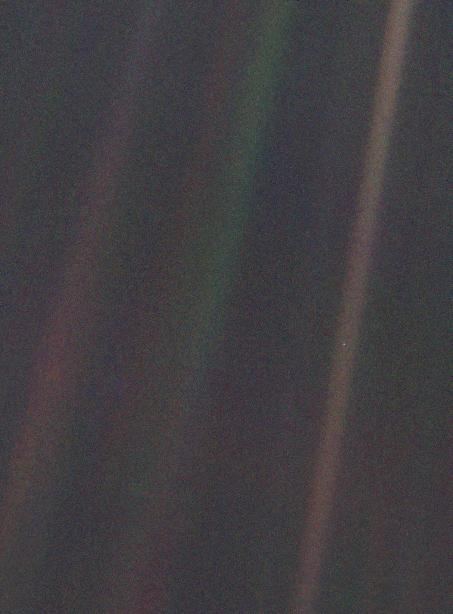
\includegraphics[width=0.95\textwidth]{figures/chapter1/fig1b_Voyager_PaleBlueDot.jpg}
\caption[Voyager 1 于 1996 年 9 月 12 日拍摄到的多色合成地球肖像照。(图片版权:NASA/JPL-Caltech)]{Voyager 1 于 1996 年 9 月 12 日拍摄到的多色合成地球肖像照\footnotemark[2]。(图片版权:NASA/JPL-Caltech)}
\label{fig:voyagerearth}
\addtocounter{footnote}{+1}\footnotetext{\url{http://photojournal.jpl.nasa.gov/catalog/PIA00452}}
\end{subfigure}
\caption{人类从太空看到的赖以居住和生存的母亲行星 --- 地球。\textbf{(a)} Apollo 17 号飞船航向月球的途中宇航员们回望并拍摄到的地球。这张图被称作「蓝宝石」,图中可以清晰的看到南半球的大气云层与被冰雪覆盖的南极点,另外还可看到非洲与亚洲大陆。\textbf{(b)} Voyager 1 航天器在距离太阳四十亿公里外拍摄到的地球。在最右侧的太阳散射光柱中,地球就只是不到一个像素的小白点,而在这颗蔚蓝的星球上曾居住并流逝着所有的人类足迹。 }
\label{fig:rwalone} 
\end{figure}
\end{savenotes}
}

此外,人们往往会从哲学角度来思考地球与生命在宇宙中普遍与否。比如原子论的宇宙
描述早已开端于古希腊与古印度。随后,意大利哲学家 Bruno 亦于 1584 年提出无穷宇
宙论:太阳与地球在宇宙中并不特殊,不计其数的其他星体也和地球相差无几(文献\citen{Bruno1584})

\begin{quote}
Onde possiamo stimare che de stelle innumerabili sono altre tante lune, altre tanti globi terrestri, altre tanti mondi simili a questo.
\end{quote}

历史一脉相承至今,随着人们对太阳系内行星与地球的运动探求愈来愈充分,也许便不难
理解搜索系外行星与系外生命为何如此举足轻重。而且从技术层面上,人类也已经有足够
的能力将「第二颗地球」与「地外生命」放入可见的未来计划中\cite{WoolfAngel1998}。

\subsection{系外行星的定义}
    
二十一世纪以前,由于对冥王星的测量并不充分,科学界从传统层面上也似乎没有必要争
论如何去界定行星。尔后,随着更多的海外天体(Trans-Neptunian Objects,简称 TNOs)
被发现,冥王星是否还是太阳系第九大行星的争辩也愈演愈烈\cite{SternMitton2005}。
终于,国际天文学联合会(International Astronomical Union,简称 IAU)于 2006 年在
「B5 决议\footnotemark[3]」中给太阳系内的行星做出如下定义:
\setcounter{footnote}{3}
\footnotetext{\url{https://www.iau.org/static/resolutions/Resolution_GA26-5-6.pdf}}

\begin{enumerate}[leftmargin=1\parindent]
\item 必须拥有围绕太阳的轨道;
\item 质量应充分大,使得其自引力足够克服刚性力,以形成(近)球外形;
\item 另外,行星必须清空轨道临近的其它天体。
\end{enumerate}

根据此定义,冥王星不再属于行星范畴,而被称作一颗矮行星。那如今观测到的近 3500 颗
\footnote{来源 NASA Exoplanet Archive \url{http://exoplanetarchive.ipac.caltech.edu/index.html},
数据库更新至 2017 年 2 月 14 日}系外行星呢?从词源学上,行星(planet)一词取名自希腊语,
那么系外行星(exoplanet)自然也该遵循上述 2006-B5 决议。然而部分系外气态巨行星
(Gas Giant)质量已经大于十个木星质量($M_\tif{J}$),此类行星的质量上限在 IAU 决议中
也并未给出。实际上,早于冥王星争辩,IAU 系外行星工作小组就已规定真实质量小于 13 
$M_\tif{J}$(或行星内部氘元素热核反应的质量下限\cite{Baraffe2003})的行星才被称作系外
行星\footnote{请查看链接 \url{http://home.dtm.ciw.edu/users/boss/IAU/div3/wgesp/}}。在本文
亦一律遵循以上两者来定义系外行星。


\subsection{系外行星扼要史} 

人类从诞生之始就默默地注视着夜空的「神行者」--- 行星。而作为专注于研究系外行星系统
的科学(Exoplanetology),其研究对象则跳脱出传统可观测的太阳系各大行星,转向了银河
系内太阳周围临近的恒星。回顾历史,这门领域的兴起也并非一蹴即成,而是融入许多先人不
停探索、试错与更新的艰辛历程。

近代系外行星搜索开始于十九世纪中页,Jacob 在对 70 Ophiuchi 的天体测量数据中找到类似
行星的信号\cite{Jacob1855},然而 Moulton 后续观测立即证否了这颗行星\cite{Moulton1899}。
在随后的一个世纪内,对木星质量的系外行星探索逐渐变得活跃,如 van de Kamp 于 1963 年
将仪器系统信号误认为一颗围绕巴纳德恒星的行星(文献 \citen{vandeKamp1963})。

另外一面,Struve 在1952 年提出短周期类木系外行星可同时通过视向速度与测光探测的设想
\cite{Struve1952}。然而科学界当时理所应当都认为木星只能处在距离主星 5 AU 轨道上,因此
需要太长的时间跨度来确认探测\footnote{一般来说,由于引力所造成的周期信号被连续确认三
个周期以上便被认为是真实的天体信号。}。不过,恒星光谱学依然在其间飞速发展,HD 114762 
被发现拥有一颗非常接近系外行星质量上限的褐矮伴星\cite{Latham1989}。

此时,来自美国的二人团队 Wolszczan 和 Frail 于 1992 年利用射电脉冲信号的周期变化率在
脉冲星 PSR1257+12 周围率先成功探测到包含两颗约 3 $M_\oplus$ 行星的行星系统
\cite{WolszczanFrail1992}。而 Walker 等人则在对主序恒星长达 12 年的视向速度监测中,
宣布没有迹象表明他们嗅探到系外木星信号\cite{Walkeretal1995}。

同一年,来自瑞士日内瓦天文台的 Mayor 和 Queloz 做出了系外行星领域里程碑式的发现(文
献\citen{MayorQueloz1995}): 他们利用坐落在法国 Haute-Provence 天文台的 ELODIE 光谱
仪从 150 颗恒星样本中成功探测到第一颗类太阳恒星周围的行星  --- 51 Peg b(见图 
\ref{fig:51pegsi})。这颗轨道周期只有 4.23 天的类木行星于同一年被美国 Marcy 和 Butler 团
组证实,随后便引起了对此类行星(即热木星)形成理论机制广泛而又深远的讨论
(\S \ref{sec:pltfrmatntheory}),一直延续至今。

\begin{figure}[ht]
\centering
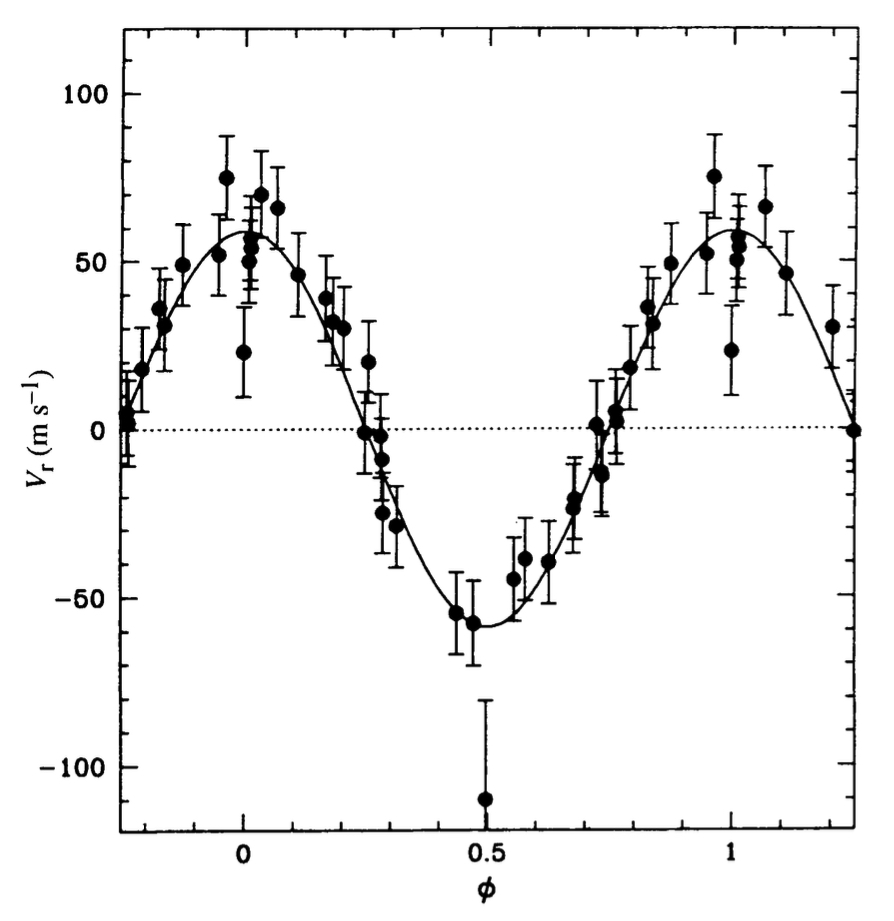
\includegraphics[width=0.95\textwidth]{figures/chapter1/fig2_51pegsi.jpg}
\caption[1995 年,日内瓦天文台天文学家 Mayor 和 Queloz 连续观测恒星 51 Pegsi 得到的视向速度曲线图,观测点已全数叠加至其伴星的周期 4.23 天。该系统主星是一颗类太阳恒星,因此视向速度曲线振幅所对应的最小质量为 0.47 $M_\tif{J}$ ,系人类首次发现到类太阳恒星周围的短周期类木行星。]{日内瓦天文台天文学家 Mayor 和 Queloz 连续观测恒星 51 Pegsi 得到的视向速度曲线图,观测点已全数叠加至其伴星的周期 4.23 天。该系统主星是一颗类太阳恒星,因此视向速度曲线振幅所对应的最小质量为 0.47 $M_\tif{J}$ ,系人类首次发现到类太阳恒星周围的短周期类木行星。图片取自他们于 1995 年发表在自然杂志的文献 \citen{MayorQueloz1995}。}
\label{fig:51pegsi}
\end{figure}

紧随其后的二十年内,系外行星领域各大新奇发现此起彼伏。图 \ref{fig:pltdiscyear} 为年度新
发现系外行星数目柱状图,该数目明显呈现出指数式增长,尤其是 2009 年 Kepler 太空望远
镜\cite{Boruckietal2010} 的发射新带来了大批通过凌星法发现的系外行星。图\ref{fig:pltdiscyear} 
中所展现的愈加多样化的样本也极大地丰富了我们对系外行星的认知。

\begin{figure}[hb]
\centering
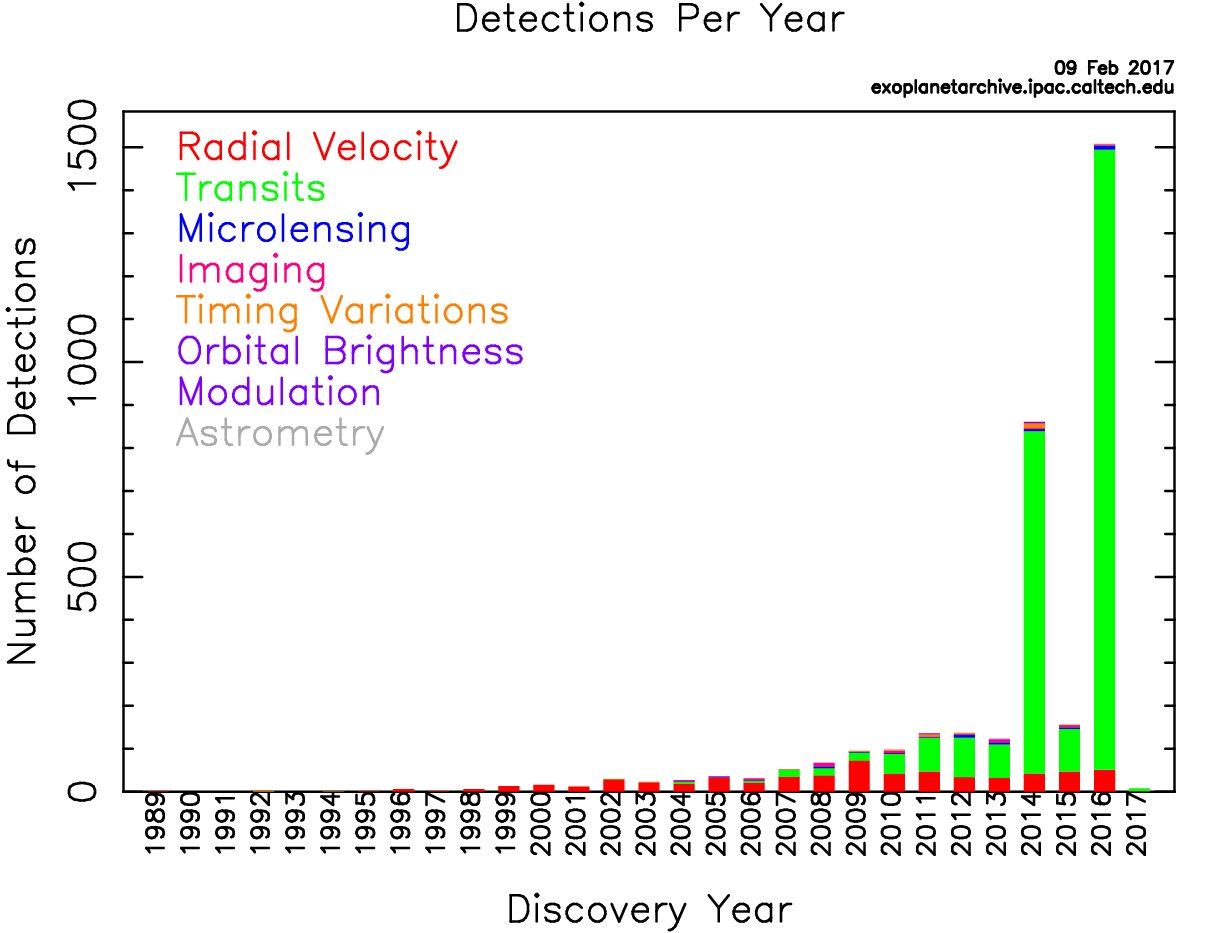
\includegraphics[width=0.95\textwidth]{figures/chapter1/fig3_nasaexo_dischist.jpg}
\caption{系外行星发现数量趋势图,不同颜色代表不同的探测方法(参照 \S \ref{sec:detmeth}),可以看出该数目呈现指数式增长。(图片取自 NASA Exoplanet Archive)}
\label{fig:pltdiscyear}
\end{figure}



\section{探测方法} \label{sec:detmeth}

天文学所研究的天体普遍离地球遥远,因而观测手段也主要集中在分析天体发射的光子上。
观测系外行星相较与恒星或太阳系内行星,通常要求非常高分辨率、灵敏度和稳定性的仪器,
也因而会遇到诸多困难,甚至还得排除恒星自身活动的干扰。比如测量围绕类太阳的系外地球
需要精度为 1 m s$^{-1}$的视向速度测量,相当于使用分辨率为 R = 100,000 的光谱仪器探测
主星光谱约 $10^{-6} \AA$ 的移动大小。参考书籍 \citen{Perryman2014exohb},本文大
致罗列目前主要探测系外行星的方法如下:

\subsection{视向速度}

假使恒星周围存在行星,那么它们便会同时绕着公共的质心(COM)做开普勒运动。在观测中,
这种三维运动可分解为视线平面内的二维运动与视线方向上的运动。视向速度(Radial Velocity,
简称 RV)法就是通过测量视线方向上恒星谱线的多普勒红(蓝)移来探测周围行星的存在。

在简单的二体运动中,可以得到一颗轨道半长径为 $a$,质量为 $M_\tif{p}$ 的行星,可对质量
为 $M_\tif{s}$ 的宿主恒星造成如下大小的半振幅视向速度 $K_1$(单位:米每秒):

\begin{equation}  \label{eq:rvk} 
K_1 \simeq \frac{28.4 }{\sqrt{1-e^2}} \frac{M_\tif{p}\sin i}{M_\tif{J}} \, \bigg(\frac{M_\tif{p}+M_\tif{s}}{M_\odot}\bigg)^{-1/2} \big(\frac{a}{1 \tif{AU}}\big)^{-1/2}
\end{equation}  %\myequations{视向速度法探测系外行星}


其中各物理量的意义参见附录\ref{apdx:twobodyproblem}。由上式可知,视向速度方法最重要的缺
陷即它只能测量(或拟合)出行星的最小质量(Minimum Mass,即$M_\tif{p}\sin i$)因为行星的轨
道倾角 $i$ 或视线方向夹角无法被测量。但与此同时,视向速度最明显优势是它可以精确测量行星
的轨道偏心率 $e$(图 \ref{fig:rvcurve} )。

\begin{figure}[h!]
\centering
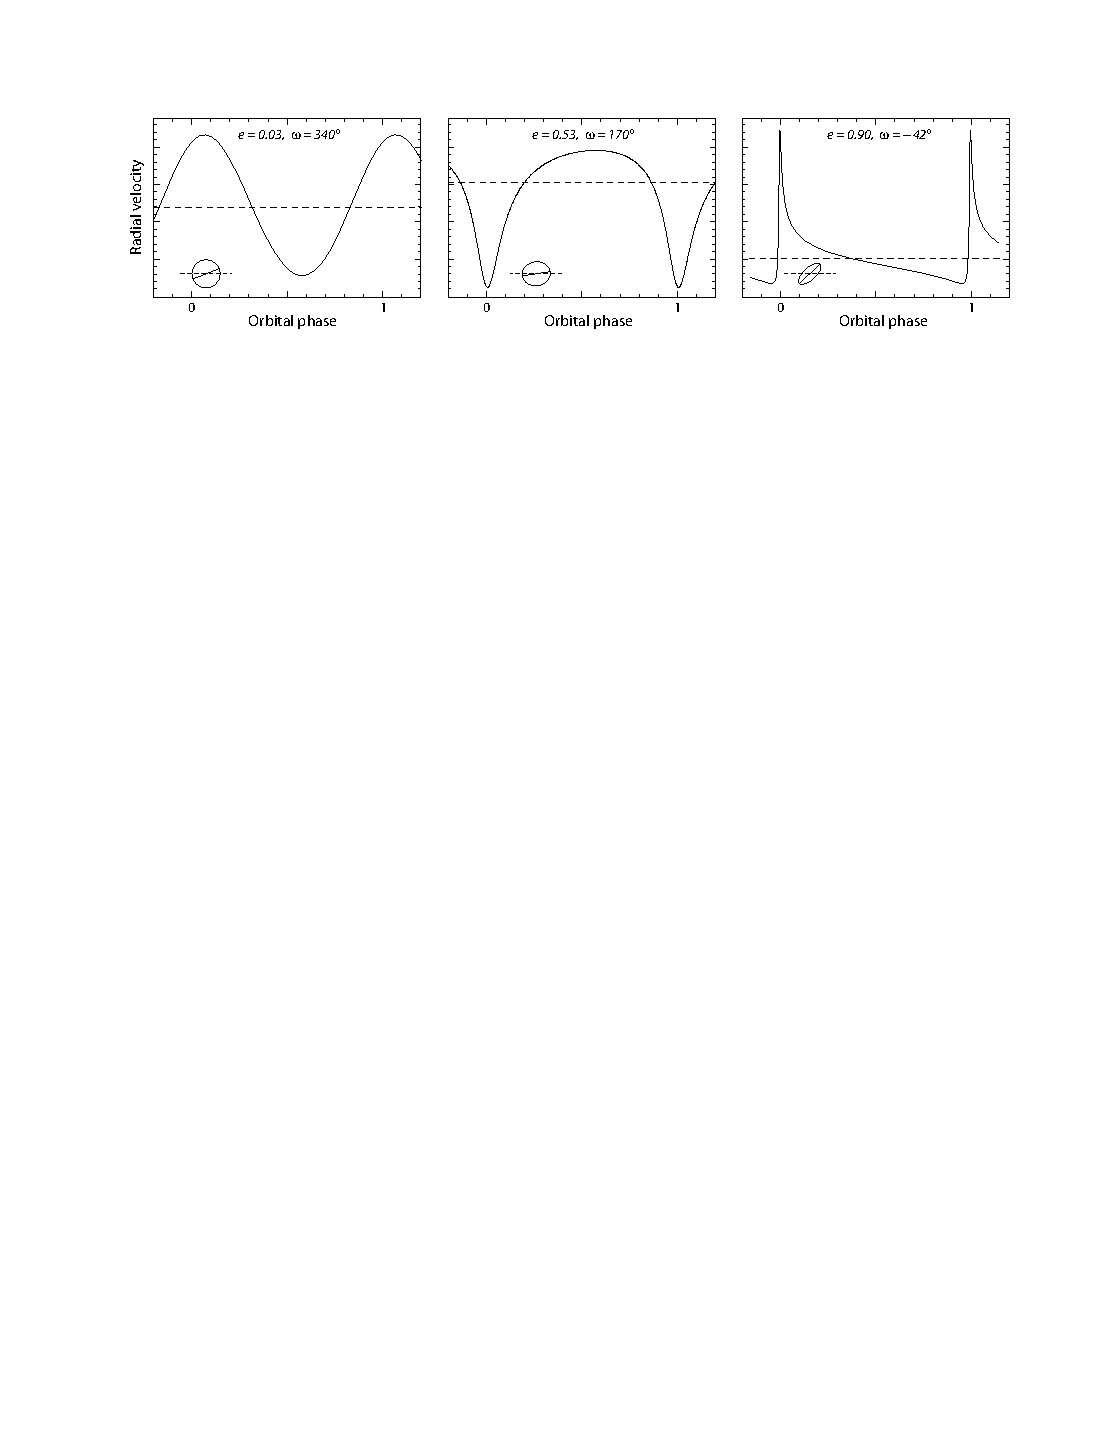
\includegraphics[width=1.0\textwidth]{figures/chapter1/fig5_rvcurve.pdf}
\caption[行星对主星造成的视向速度曲线示意图,从左至右分别代表不同的行星偏心率和轨道近心点取向。此图版权归 Perryman M. 所有。]{行星对主星造成的视向速度曲线示意图,分别代表不同的行星偏心率和轨道近心点取向。从左至右分别示意系统 HD 73256\cite{Udry2003HD73256},HD 142022\cite{Eggenberger2006HD142022} 和 HD 4113\cite{Tamuz2008HD4113}。此图取自文献 \citen{Perryman2014}。}
\label{fig:rvcurve}
\end{figure}

另外由于视向速度需要通过尽可能多的主星谱线来确认谱线的位移,因而往往更容易探测到 FGKM 
型主序星附近的大质量行星。在这里值得一提的是,由 Murphy 等人提出的激光频率梳法\cite{Murphyetal2007lasercomb}
与 Molecule Iodine Cell 或 ThAr Lamps 等传统的光谱仪器定标方法相比,可以更稳定重复的覆盖同
样的谱线区间,因此未来在视向速度方法上有相当可观的应用前景。

%优缺点,国际主流望远镜和团队?

\subsection{凌星法}

从原理上来说,凌星法是通过测量行星遮挡主星时主星亮度(流量)的变化来探测行星的。如图
 \ref{fig:transit} 所示,系外行星处于恒星与地球的连线时被称作凌星( Transit)或主掩食(Primary 
Eclipse),而当恒星处于系外行星与地球的连线时则被成为掩星(Occultation)或次掩食
(Secondary Eclipse)\footnote{凌星被约定特指半径较小天体遮挡大天体,而掩星则相反。双星中
的掩食通常只用于大小相近天体的互相遮挡}。

\begin{figure}[ht]
\centering
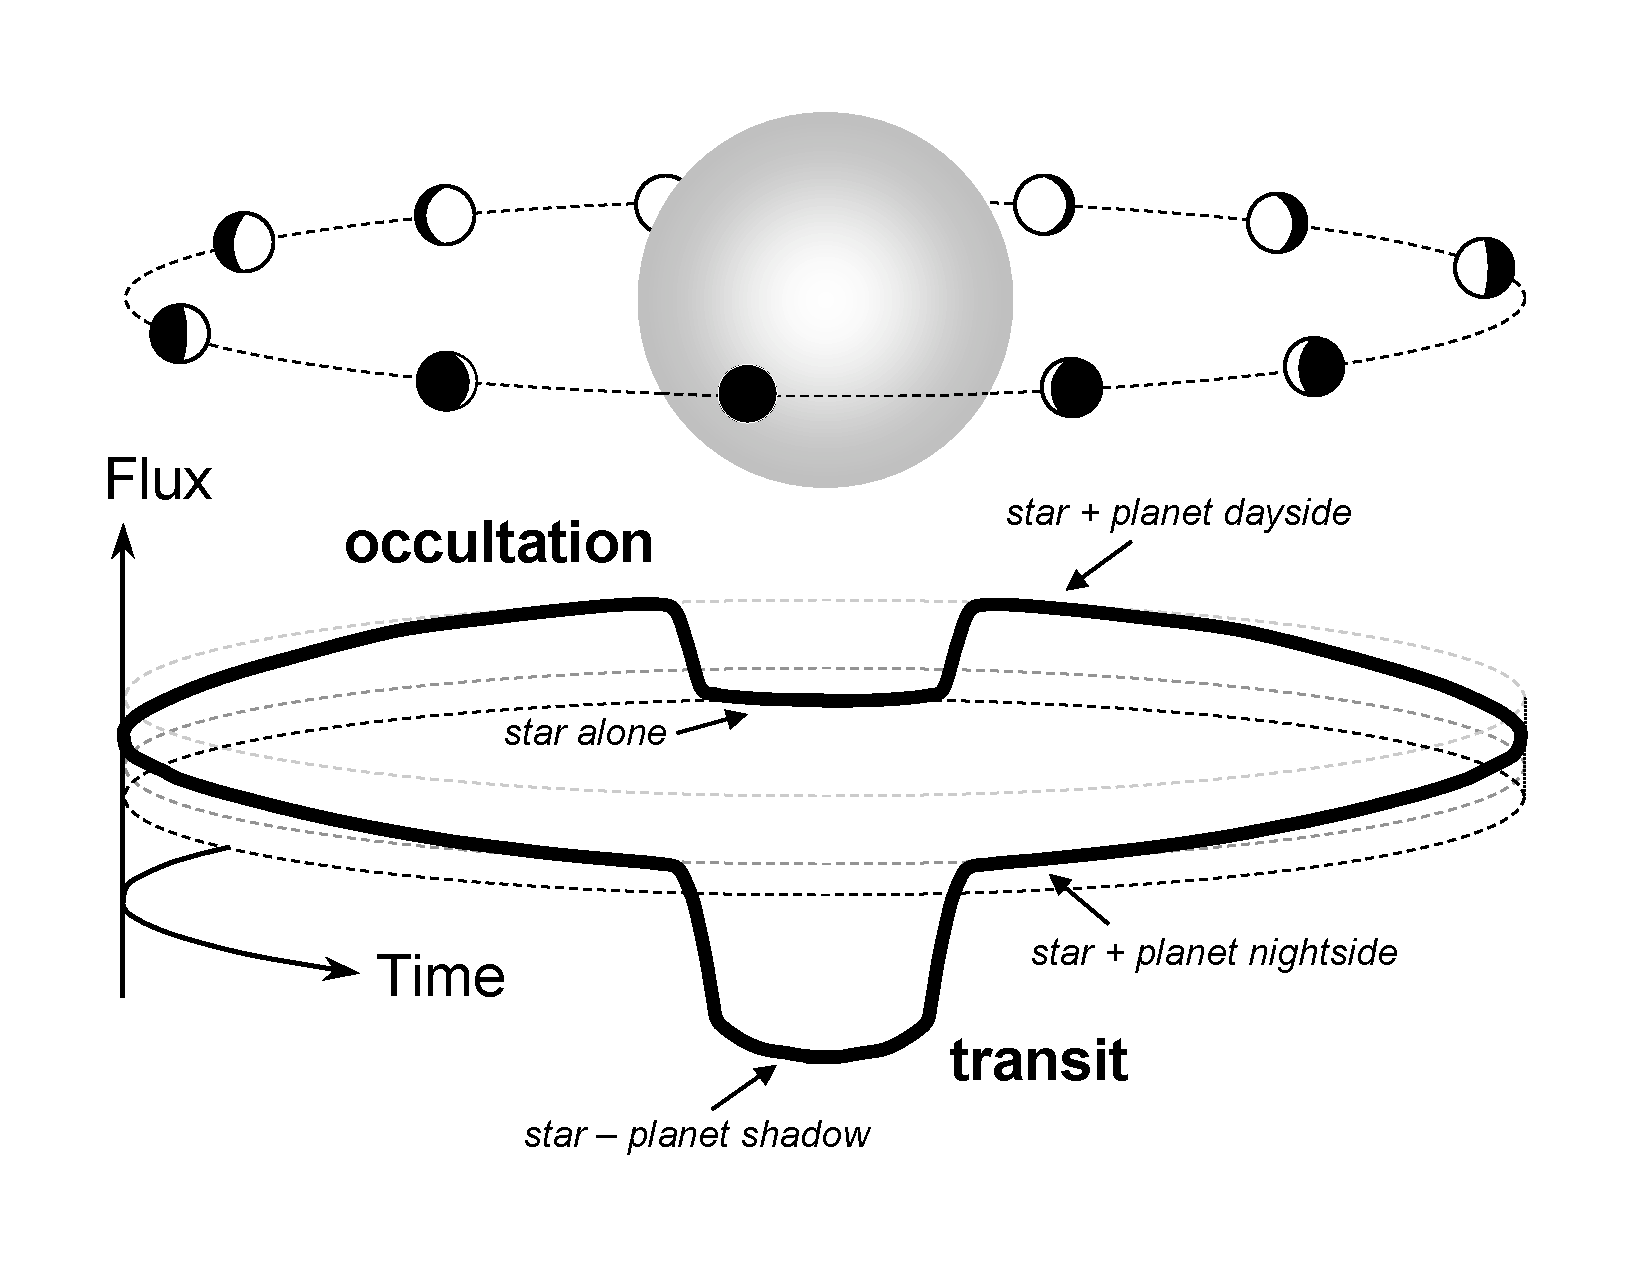
\includegraphics[width=0.95\textwidth,angle=-90, trim={0 1cm 0 0}, scale=0.9]{figures/chapter1/fig6_transit.pdf}
\caption[凌星法探测行星示意图,上半部分表示不同的轨道时刻。下方则为整个系统观测到的流量变化。版权 Joshua Winn。]{凌星法探测行星示意图,凌星法探测行星示意图,上半部分表示不同的轨道时刻。下方则为整个系统观测到的流量变化。此图取自书籍 \citen{Seager2010exobook}。}
\label{fig:transit}
\end{figure}

事实上,掩食在太阳系内已属屡见,比如日、月食和金星凌日现象。虽然凌星法探测与视向速度
法在原理上被 Struve 于同一年提出\cite{Struve1952},但真正意义上的第一次观测到系外凌星却
比视向速度晚了五年\cite{Seager2010exobook}。当时视向速度已经发现了 64 颗系外行星,在对
其中 6 颗行星系统的凌星监测中,行星 HD 209458 b 的主掩食成功被观测到\cite{Henryetal2000, Charbonneauetal2000}。
这种滞后主要是因为凌星发生的几何空间概率较低($p = R_\tif{s} / a$),与此同时还要求观测的
相对测光精度至少达到 5 \textperthousand(对应于木星凌太阳),凌星法也因此通常结合巡天计
划(尤其是大视场巡天)展开,因而提高测光精度、处理数据和去除假阳性信号也成了该方法的技
术难关\footnote{凌星法只能得到系外行星的候选体,一般还需额外使用其他方法联合认证该行星,
如中天时刻变化(Transit Timing Variation,简称 TTV)或者 RV。}。目前地面上比较成熟的巡天项
目,包括 The Trans-atlantic Exoplanet Survey(TrES)\cite{Alonsoetal2004TrES},XO
\cite{McCulloughetal2005XO},The Hungarian-made Automated Telescope Network(HAT)
\cite{Bakosetal2007HAT} 以及 Wide Angle Search for Planets(SuperWASP)
\cite{Pollaccoetal2006WASP},相应的空间巡天项目也有 Convection, Rotation and planetary 
Transits(CoRoT)\cite{Bargeetal2008CoRoT} 与 Kepler\cite{Boruckietal2010}。


\subsection{天体测量}

\begin{figure}[h!]
\centering
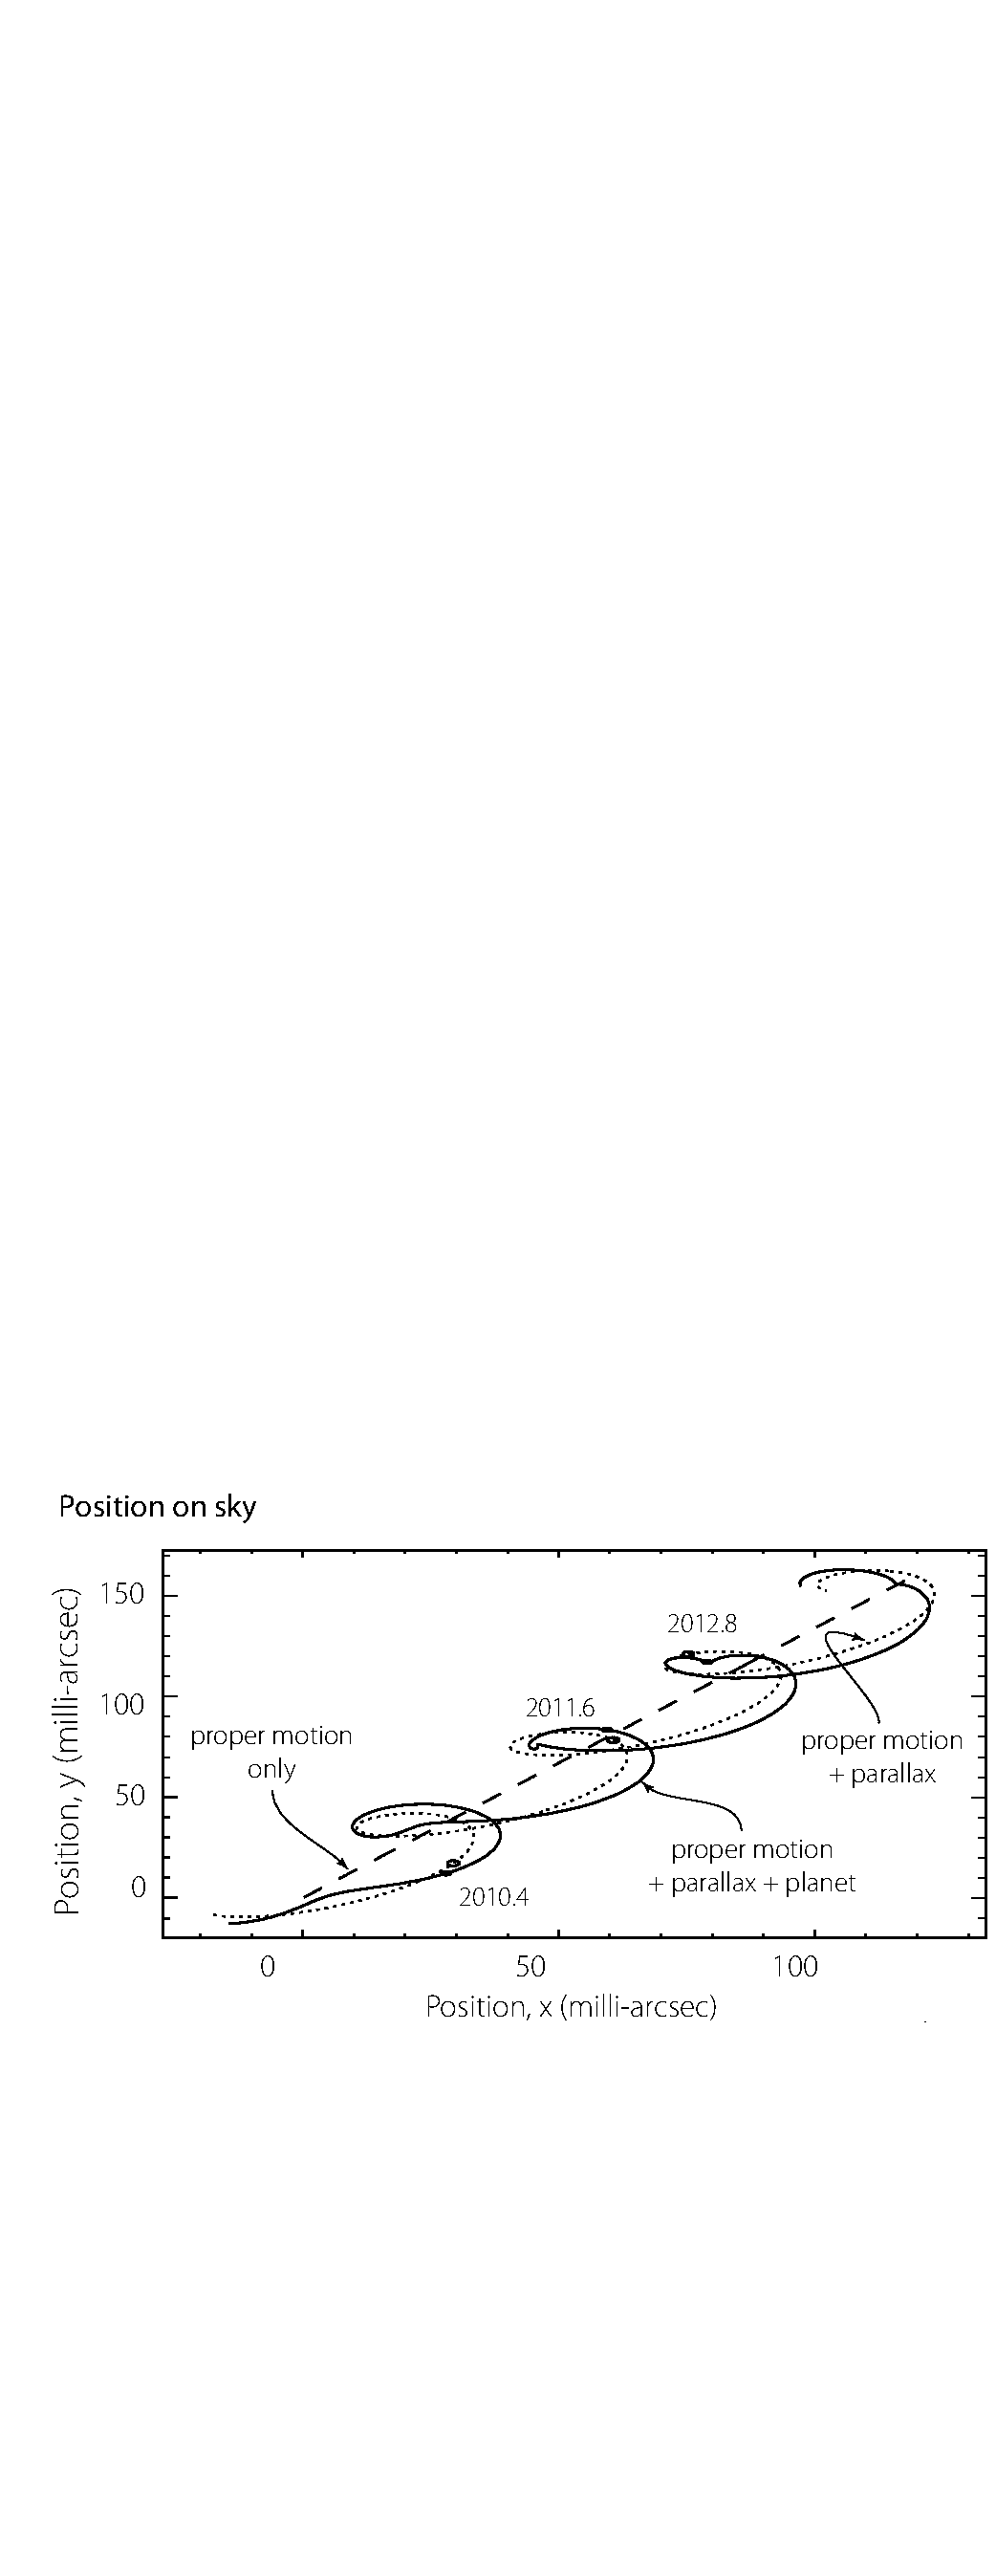
\includegraphics[width=0.95\textwidth]{figures/chapter1/fig7_astrometry.pdf}
\caption[由于行星的存在,宿主恒星的天球坐标随着时间的变化示意图,版权所有:Perryman M。]{由于行星的存在,宿主恒星的天球坐标随着时间的变化示意图。此图取自文献 \citen{Perryman2014}。}
\label{fig:astrometry}
\end{figure}

和视向速度探测主星前后摆动不同,天体测量法(Astrometry)着重于观测恒星在天球上的左右摆
动。行星对宿主恒星造成的来回振幅大小可用如下公式估算

\begin{equation}  \label{eq:astrometry} 
\alpha \simeq \bigg(\frac{M_\tif{p}}{M_\tif{s}}\bigg) \, \big(\frac{a}{1 \tif{AU}}\big) \, \bigg(\frac{d}{1 \tif{pc}}\bigg)^{-1} \tif{arcsec}
\end{equation} %\myequations{天体测量法探测系外行星}

如图 \ref{fig:astrometry} 所示,天体测量法只需要恒星在天球球面上的经度纬度信息就可探测到
行星,它也对主星的性质没有任何依赖,因而有其独特的优势,如可探测轨道倾角参数 $i$。
2013 年,Gaia 天体测量卫星成功发射,虽然目前来看科学数据尚未达到探测系外行星的精度
\cite{GaiaCo2016},期待今后几年会有振奋人心的成果。


\subsection{直接成像}  \label{sec:drctimgmeth}
中国古话有道是「耳听为虚,眼见为实」,直接成像法便可把行星直观地展示出来。技术上这其实
并非易事:距太阳系几十个秒差距以外的行星与其主星的空间张角(Angular Separation)往往远
小于望远镜分辨率。即使空间上能分辨,恒星的黑体辐射也往往比行星高近十个量级(图 
\ref{fig:contrast})。在实际的观测中,对行星直接成像往往需要星冕仪(Coronagraph)或干涉仪
(Interferometer)的辅助(如图 \ref{fig:hr8799})。

\begin{figure}[h]
\centering
\begin{subfigure}[b]{.48\textwidth}
\captionsetup{width=0.9\textwidth}
\centering
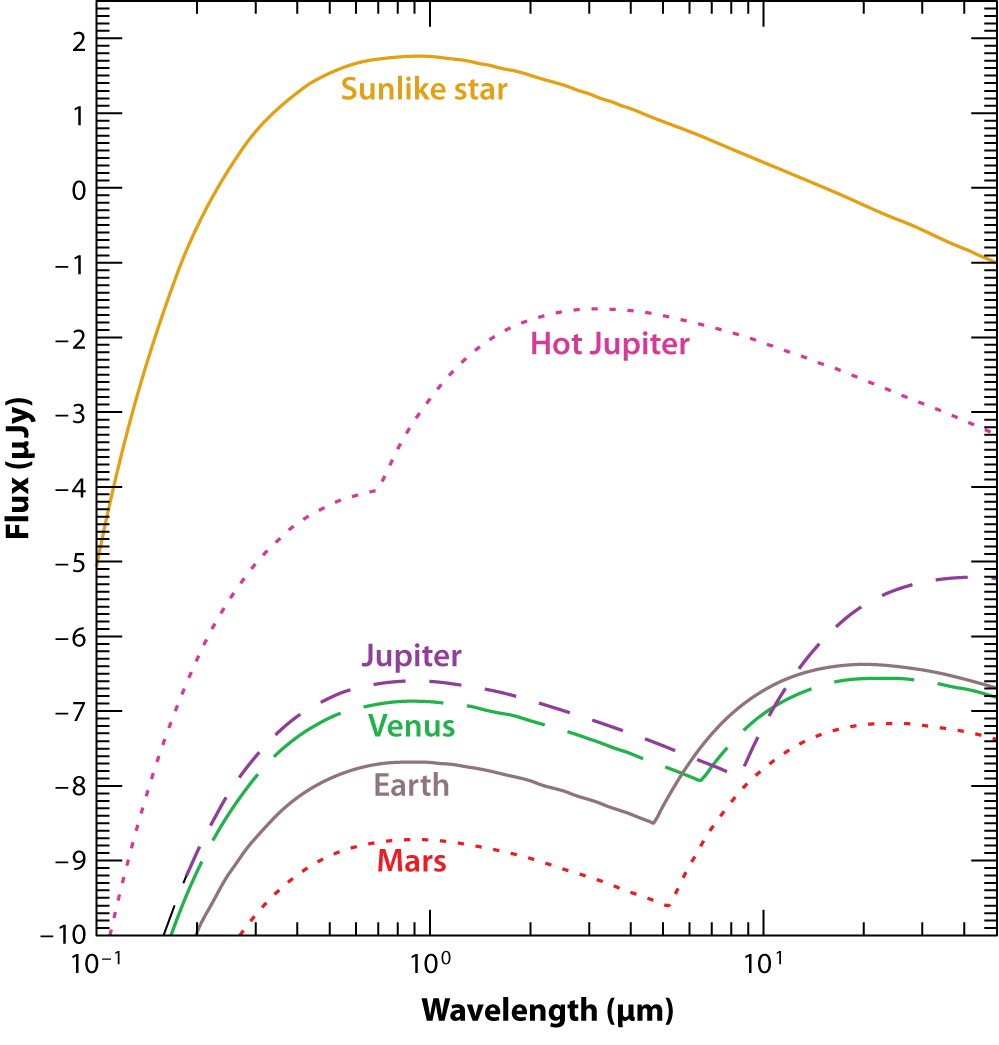
\includegraphics[width=0.95\textwidth]{figures/chapter1/fig8a_dicontrast.jpg}
\caption[仪器接受类太阳恒星在 10 pc 以外的黑体辐射(黄色实线),其余为太阳系行星与热木星在此恒星周围黑体发射与发射的叠加流量。在可见光波段行星与主星的对比度可差至十个量级,因此直接成像法一般选择在长波范围(如红外波段)探测系外行星。图片版权 Seager and Deming。]{可见光波段行星与主星的对比度可差至十个量级,因而直接成像法一般选择在长波范围(如红外波段)观测系外行星。图片摘自文献\citen{Seager2010}。}
\label{fig:contrast}
\end{subfigure}
\begin{subfigure}[b]{.48\textwidth}
\captionsetup{width=0.9\textwidth}
\centering
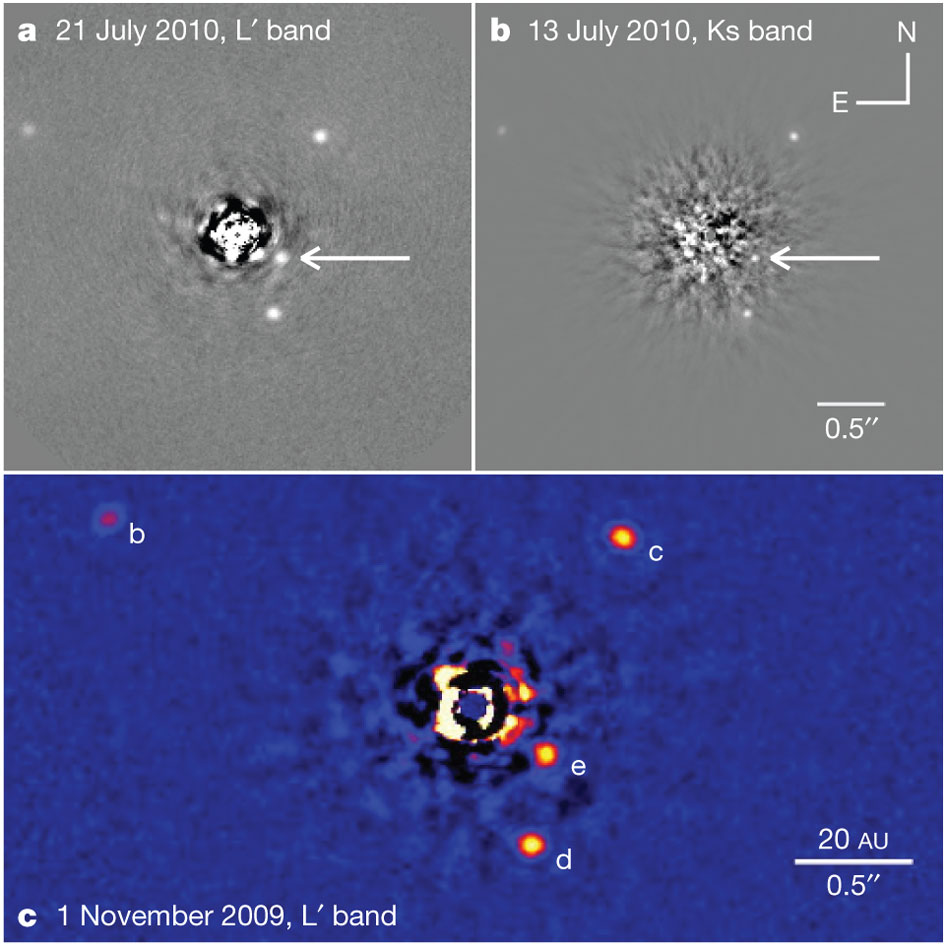
\includegraphics[width=0.95\textwidth]{figures/chapter1/fig8b_hr8799.jpg}
\caption[Keck 望远镜利用角向较差成像与自适应光学技术在近红外波段通过直接成像得到的 HR 8799 系统。中心恒星的大部分光已被星冕仪遮挡,留下小部分噪声,与远处四颗行星 。图片版权:Marois 等人。]{Keck 望远镜在近红外波段通过直接成像得到的 HR 8799 系统。中心恒星的大部分光已被星冕仪遮挡,留下小部分噪声,与远处四颗行星 。图片取自文献\citen{Marois2010}。}
\label{fig:hr8799}
\end{subfigure}
\caption{直接成像法探测系外行星。\textbf{(a)} 仪器接受类太阳恒星在 10 pc 以外的黑体辐射强度,其余为太阳系行星与热木星在此恒星周围黑体发射与发射的叠加流量。\textbf{(b)} Keck 望远镜利用角向较差与自适应光学技术直接成像观测到的 HR 8799 系统。}
\label{fig:directimage} 
\end{figure}

直接成像方法往往偏向于探测年轻的系统,如 HR 8799\cite{Marois2008HR8799}, 
Fomalhaut\cite{Kalas2008} 和 $\beta$ Pictoris\cite{Lagrange2010},这是因为行星在其形成早期会
拥有较强的近红外辐射。目前用于此方法的望远镜有 Hubble Space Telescope(HST),Keck,
Very Large Telescope(VLT)和 Gemini Planet Imager(GPI)等
\cite{Marois2008HR8799,Chauvin2005,Macintosh2014}。

\subsection{其他方法}
\textbf{微引力透镜(Microlensing):} 本方法原理可以追溯到 1936 年,Einstein 发表了一篇
计算前景星对视线方向上背景星引力放大率的文章\cite{Einstein1936}。而且在第一颗用微引力透镜
观测得的行星前,Mao 和  Paczynski 就已经从理论上提出了行星能在恒星引力透镜基础上造成额外
的微引力透镜效\cite{Mao1991}。如今已经有 42 个通过微引力透镜发现的系外行星系统,包括 2 个
双行星系统\footnote{参见 NASA Exoplanet Archive:\url{http://exoplanetarchive.ipac.caltech.edu/}}。
在役的仪器主要有 Optical Gravitational Lensing Experiment(OGLE)\cite{Udalskietal2002OGLE} 
和 Microlensing Observations in Astrophysics(MOA)\cite{Bond2004MOA},它们一般会监测恒星
密度较大的区域如银河系核球(Galactic Bulge)。

\textbf{计时法(Timing):} 传统计时法最典型的例子就是最早被发现的系统 --- 脉冲星 
PSR1257+12 行星系统\cite{WolszczanFrail1992}。除了传统的 Pulsar Timing Variation 之外,可以
说任何理论上拥有稳定周期信号的恒星计时变化都可以用来探测潜在的系外行星:如凌星计时变化 
TTV\cite{Ford2011TTV,Xie2013} 和星震时变\cite{Silvotti2007,Murphy2016}。此方法应用前景也非
常可观,特别是针对多行星系统动力学特征刻画\cite{HolmanMurray2005}。

除此以外,Perryman 列出了更为系统且详细的探测方法,对应的探测能力以及它们在将来可能的应
用\cite{Perryman2000},请参见下页图 \ref{fig:detmethod}。

\begin{sidewaysfigure}
    \centering
    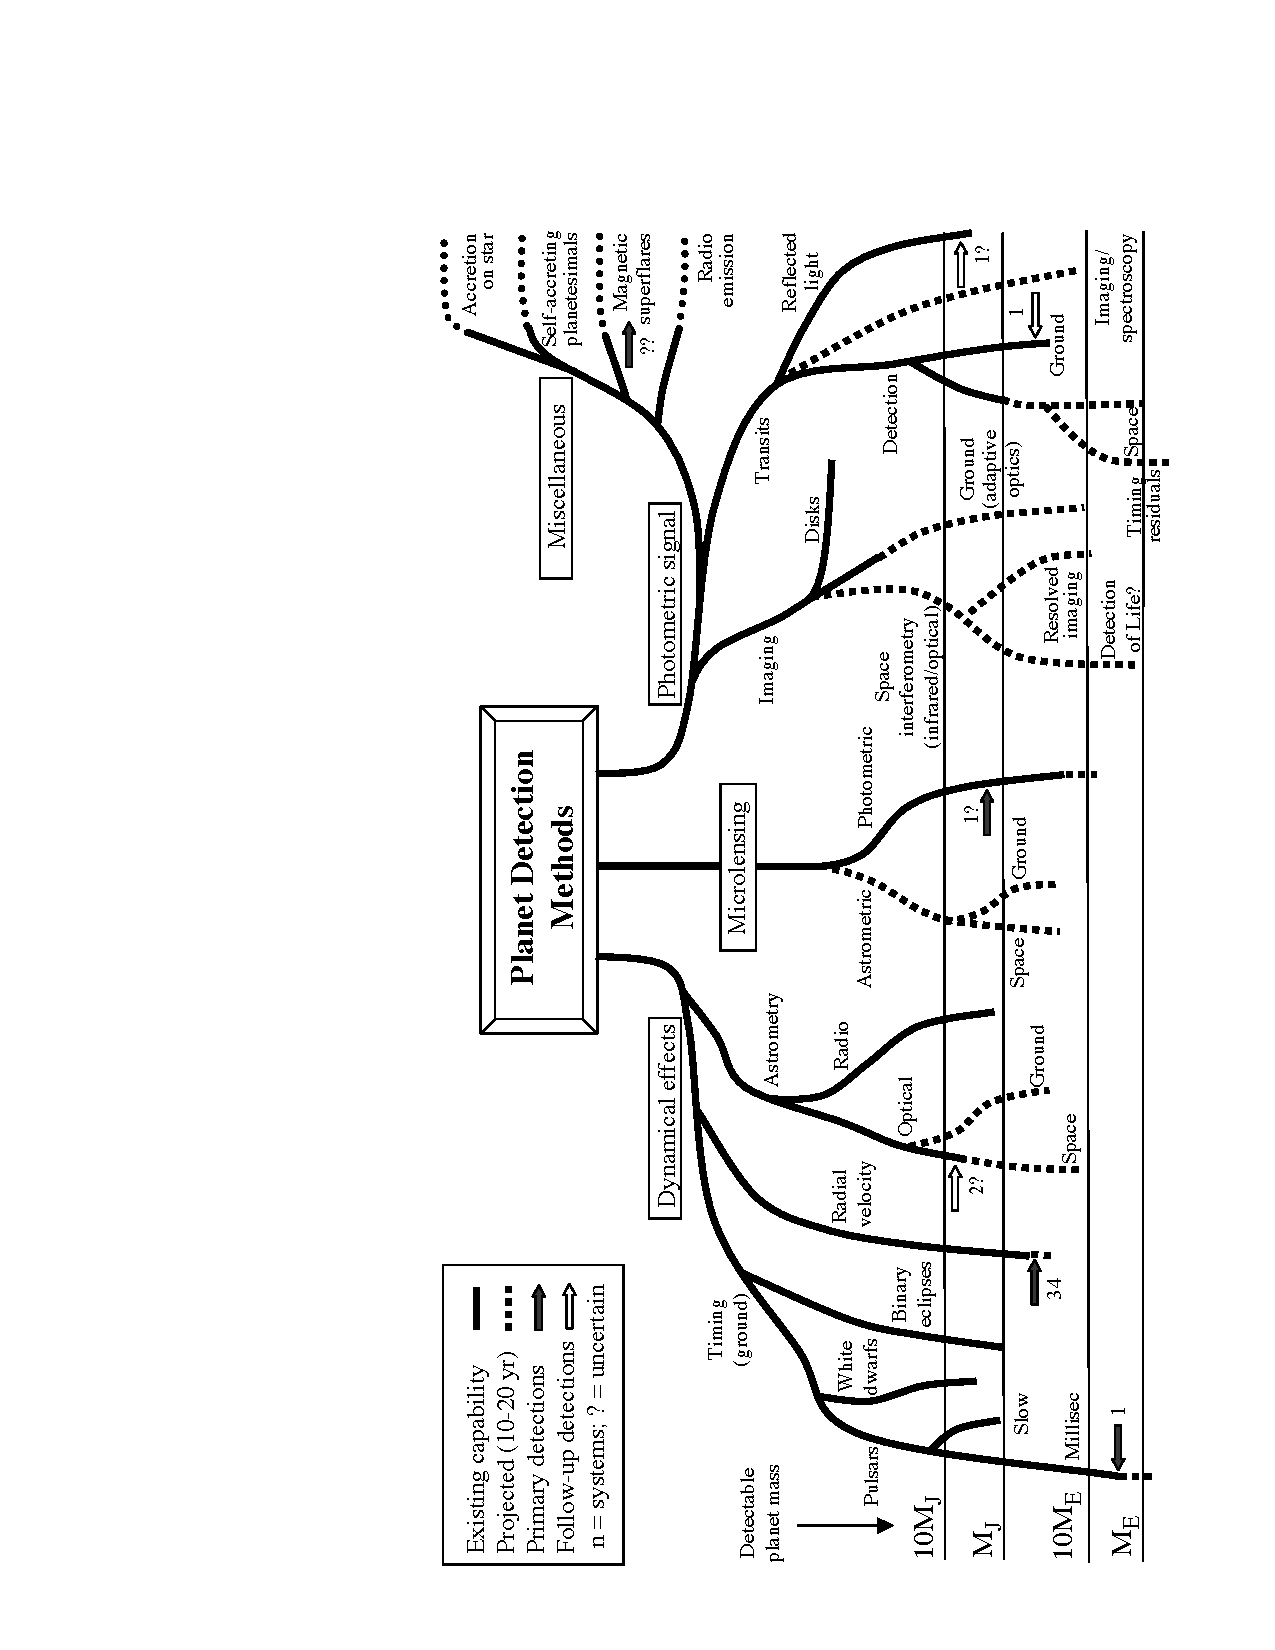
\includegraphics[scale=0.95, angle=-90]{figures/chapter1/fig4_fmethods.pdf}
    \caption[系外行星探测方法大全,图片版权 Michael Perryman。]{系外行星探测方法大全,关于图片说明请参见文献\citen{Perryman2000},此图摘录自该文献的第一幅插图。}
    \label{fig:detmethod}
\end{sidewaysfigure}


\section{行星形成理论} \label{sec:pltfrmatntheory}


星际空间并不是空无一物的,英国天文学家 William Herchel 在 18 世纪末观测到恒星周围冷暗物质
吸收带,我们的原太阳就是在这般空间环境中孕育而成\cite{Spitzer1978}。随着原初分子云坍缩,
核心区域会演化成原恒星,而周围的物质会由于原初角动量守恒而沉降成盘状结构以及双极喷流
(Bipolar Jets),比如观测到的 Herbig-Haro 型天体\cite{Lequeux2005}。

在恒星形成的早期,现有的观测证据主要集中在 T-Tauri 型天体上(又叫 Young Stellar Objects,
简称 YSOs)。YSOs 通常会按照红外谱指数($\alpha_\tif{IR} = \d\log \lambda F_\lambda)/(\d\log \lambda$)
分为 Class 0,Class \RN{1}, Class \RN{2}, Class \RN{3} 四种类型\cite{Andreetal2000}(见图
 \ref{fig:ysostage}),它们恰恰各自对应着不同的原恒星演化阶段。

\begin{figure}[t]
\centering
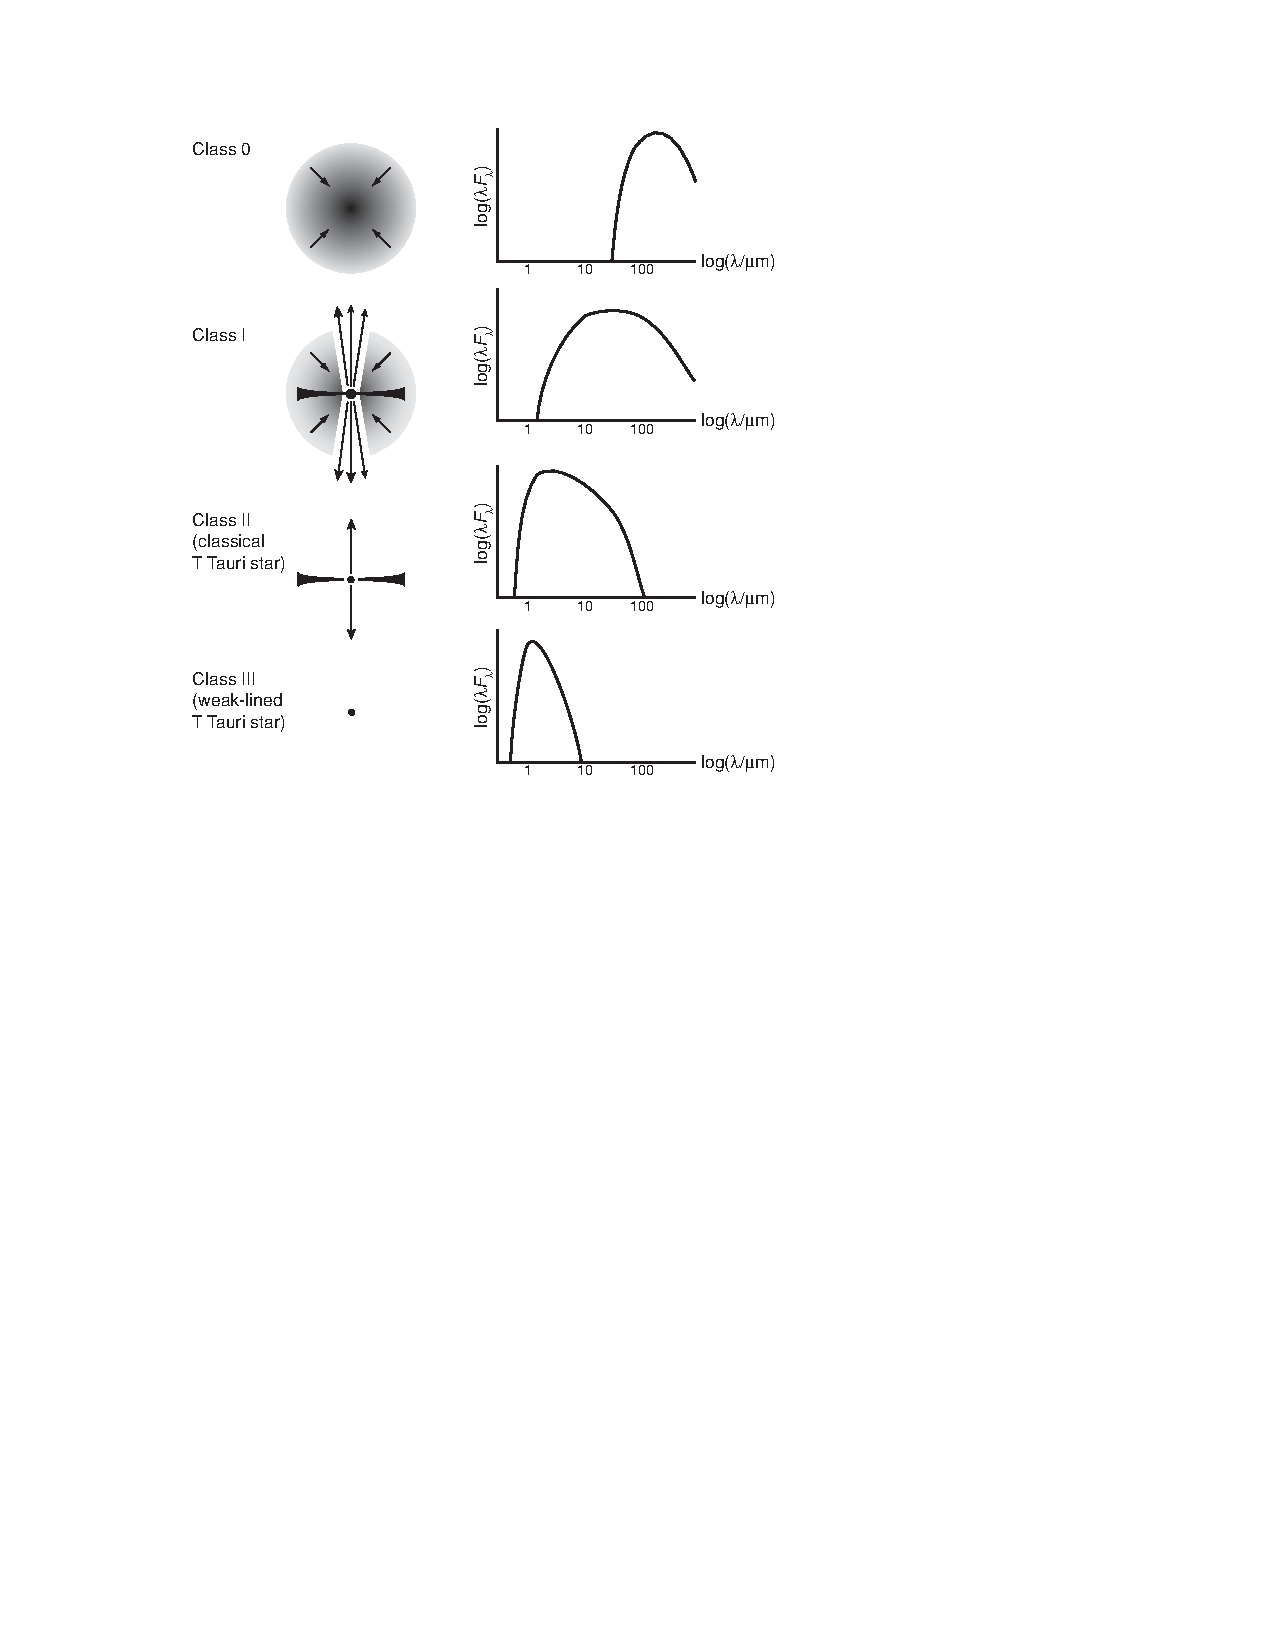
\includegraphics[width=0.95\textwidth]{figures/chapter1/fig9_ysostages.pdf}
\caption[YSOs 按照红外谱指数划分的四种主要类别,版权所有:Armitage P.。]{YSOs 按照红外谱指数划分的四种主要类别,图中背离黑体谱的红外突起部分又被称作红外超,它也是恒星是否存在盘的重要判据之一。此图取自书籍 \citen{Armitage2010}。}
\label{fig:ysostage}
\end{figure}

从某种程度上说,此刻的原恒星盘(Protostellar Disk)已可被称作原行星盘
\footnote{一般而言在恒星形成的早期,当恒星处于活跃吸积阶段时星周盘被称作原恒星盘,
而在随后的行星形成阶段则被称作原行星盘。}(Protoplanetary Disk)。
根据文献\citen{Armitage2007},由于恒星对周围气体的吸积\cite{Pringle1981}、恒星的高能辐射
\cite{Johnstone1998,Hollenbach1994},以及气体盘自身的粘滞性
\cite{Shakura1973,Gammie1996},角动量会从从气体盘的内侧向外转移,原行星盘也会
逐渐耗散。2001 年,Haisch 等人通过统计不同星团中的红外超恒星比例,发现原行星盘的存活时标
在不到百万年(~10 Myr)的量级\cite{Haisch2001}。这对类木行星行形成有着非常重要的限制,因
为如今普遍认为木星必须在气体盘消散前吸收足够的气体来长成如今的质量大小\cite{WilliamsCieza2011}。

\begin{figure}[t]
\centering
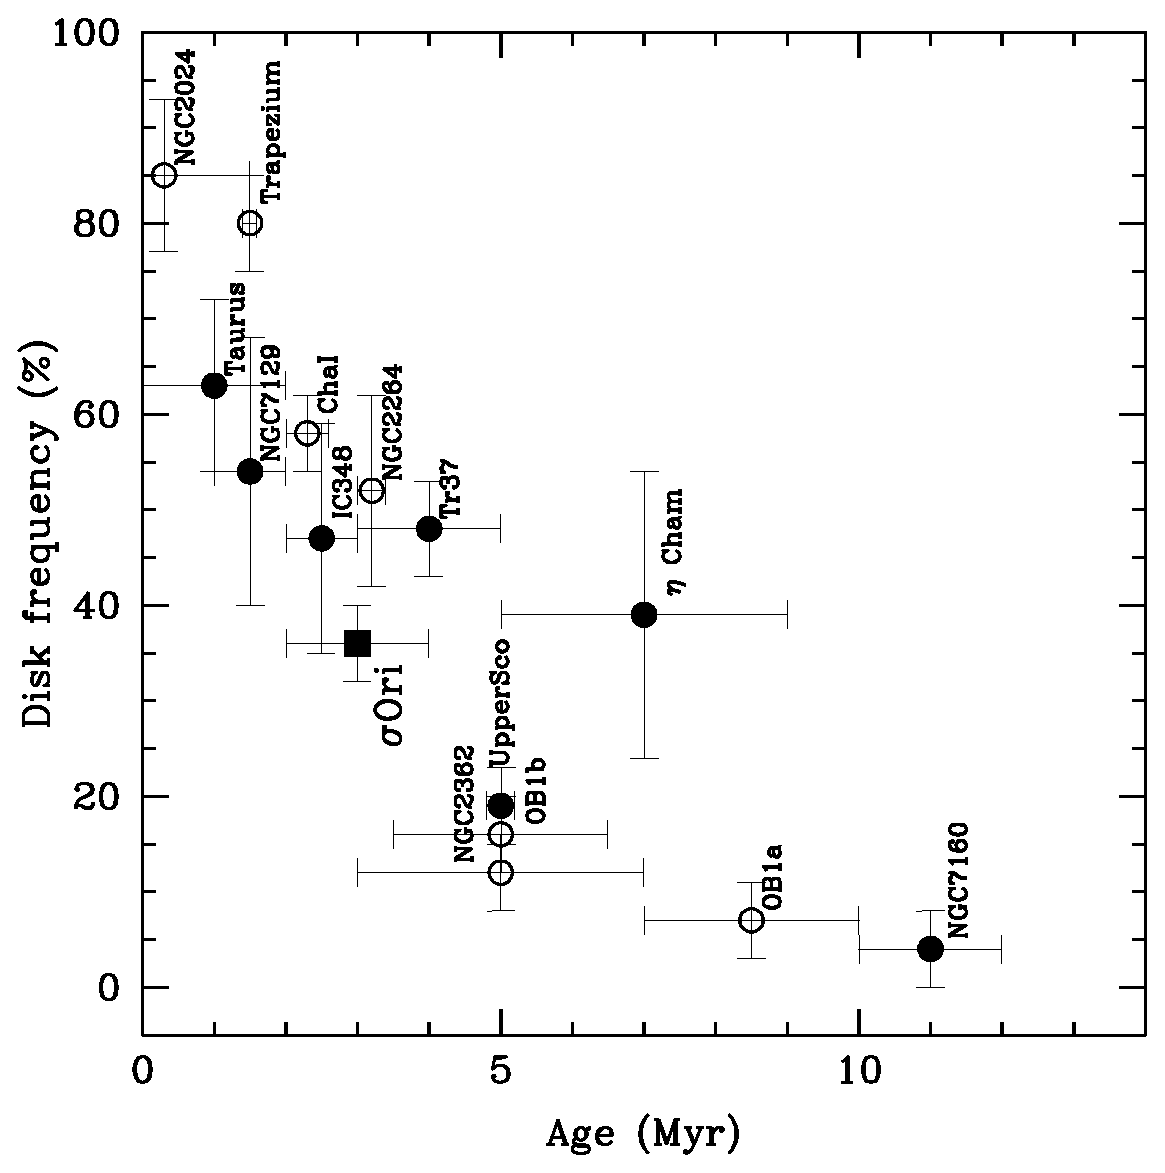
\includegraphics[width=0.95\textwidth]{figures/chapter1/fig10_pftimescale.eps}
\caption[不同星团红外超等效的原(恒)行星盘站所有星团成员的比例。此图可推断星团年龄老于10 Myr 后,恒星周围的气体盘已近乎完全消散。此图版权所有:Hern{\'a}ndez J. 等人。]{不同星团红外超等效的原(恒)行星盘站所有星团成员的比例。此图可推断星团年龄在 5 Myr 左右,恒星周围的气体盘已近乎消散。此图取自文献 \citen{Hernandez2007}。}
\label{fig:ysostage}
\end{figure}

\subsection{基于太阳系的经典形成理论} \label{sec:clspftheory}

早在 18 世纪中页,关于行星形成假说就已纷繁多样。其中康德、拉普拉斯等人提出的「星云假说」
因可较好应用至太阳系行星系统中而发展壮大。表\ref{tbl:solarsystem} 给出了太阳系八大行星的物
理参数,由此表可得出太阳系各大行星具有非常好的一致共面性,除了水星以外都处于近圆轨道,
且在火星和木星之间存在明显的物理性质差异。如果将每个行星的重元素平均到打散至行星之间的
空隙中,并且混入适量的氢、氦使得新的混合物拥有与太阳相等的金属丰度
\footnote{在天文学中,金属元素特指氢和氦以外的所有重元素。}([Fe/H]),这样得到的最小质量
原太阳行星盘被称作 Minimum Solar Mass Nebula\cite{Weidenschilling1977,Hayashi1981},
MMSN 气体盘的面密度拥有如下的幂率函数形式:

\begin{equation} \label{eq:mmsng}
\Sigma_g = 1.7 \,\times10^3 \, \bigg(\frac{r}{\tif{AU}}\bigg)^{-3/2}  \tif{g} \,\tif{cm}^{-2}
\end{equation} %\myequation{最小质量太阳星云气体面密度分布表达式}

相应的固体盘的面密度分布同样可描述为:

\begin{equation} \label{eq:mmsns}
\Sigma_s = 7.1 \, f_\tif{ice} \, \bigg(\frac{r}{\tif{AU}}\bigg)^{-3/2}  \tif{g} \,\tif{cm}^{-2}
\end{equation} %\myequation{最小质量太阳星云固体面密度分布表达式}

其中 $f_\tif{ice}$ 为雪线因子。在距离太阳 2.7 AU 以外,水分子等会凝结成冰雪等固体物质,因而
此因子会从 1 增加至约 4.2\cite{IdaLin2004}。从此最小太阳星云模型出发,假若在垂直方向上给它
一个标高使其变为三维盘,这就是经典太阳系行星形成模型的开端。根据文献 
\citen{Dullemond2005},重元素物质(以微米到厘米级尘埃形式存在)会最先开始在垂直方向上沉
降到盘的中平面;紧接着固体物质(Dust)开始碰撞结合
\cite{ppvibook2014,Weidenschilling1997,BlumWurm2008}或引力坍缩
\cite{Safronov1972,GoldreichWard1973,YoudinShu2002,ChiangYoudin2010}成星子(Planetesimal)。

\begin{table}[t]
\centering
\caption{太阳系八大行星物理参数与轨道参数,轨道根素值依照 J2000 平赤道参考系,数据取自 NASA/JPL 网站。}
\label{tbl:solarsystem}
\begin{tabular}{cccccccc}
\hline \hline
  & $a$(AU) & $P$(days) & $M_\tif{p}$($M_\oplus$) &  $e$ &  $i$(deg) &  $R_\tif{p}$($R_\oplus$) & $\rho$(g cm$^{-3}$) \\ \hline
水星        &   0.3871    &   88.0      &  0.0553    & 0.2056  &  7.00    &   0.383   &   5.427      \\
金星        &   0.7233    &   224.7    &  0.815      & 0.0068  &  3.39    &   0.949   &   5.243      \\
地球        &   1.000      &   365.2     &  1            & 0.0167 &   0.00    &   1          &   5.514      \\
火星        &   1.524      &   687.0     &  0.107     & 0.0934 &   1.85    &   0.532   &   3.933      \\
木星        &   5.203      &   4331      &  317.8     & 0.0484  &  1.30    &   11.2     &   1.326      \\
土星        &    9.537     &   10,747   &  95.2       & 0.0539 &    2.49   &   9.45     &   0.687      \\
天王星     &   19.19     &    30,589   &  14.5       & 0.0473 &   0.77    &   4.01     &  1.271       \\
海王星     &   30.07     &    59,800   &  17.1       & 0.0086 &    1.77   &    3.88    &  1.638       \\
\hline \hline
\end{tabular}
\end{table}

在 MMSN 模型下,星子的半径大概为公里量级。这样大小的星子和尘埃性质不同,它可以脱离气体
的阻尼力并通过自引力保持其结构。此时星子相互之间的引力作用变得显著,它们会经过雪崩增长与
寡头生长两个时期成长为原行星\cite{Greenberg1978,Kokubo1996,Rafikov2003,Lissauer1993}。原
行星(亦称做行星胚胎)会在接下来分别演化成气态巨行星和类地行星,其中形成气态巨行星一般被
认为通过核吸积模型(Core Accretion)形成\cite{Mizuno1980,BodenheimerPollack1986,Pollack1996},
而类地行星则需要经历更多的动力学作用过程才能形成\cite{Chambers1998}。

当然,行星形成也还存在很多问题与挑战,解释太阳系太行星还存在许多难关
\cite{Walsh2011,Morbidelli2005},数值模拟如 Nice 模型\cite{Gomes2005Nice}也并不能解释太阳系
细节构型(尤其是水的来源\cite{Raymond2009}),本文仅能作粗略介绍,图 \ref{fig:pfstage} 为上
述经典形成模型的核心各阶段过程的总结。

\begin{figure}[t]
\centering
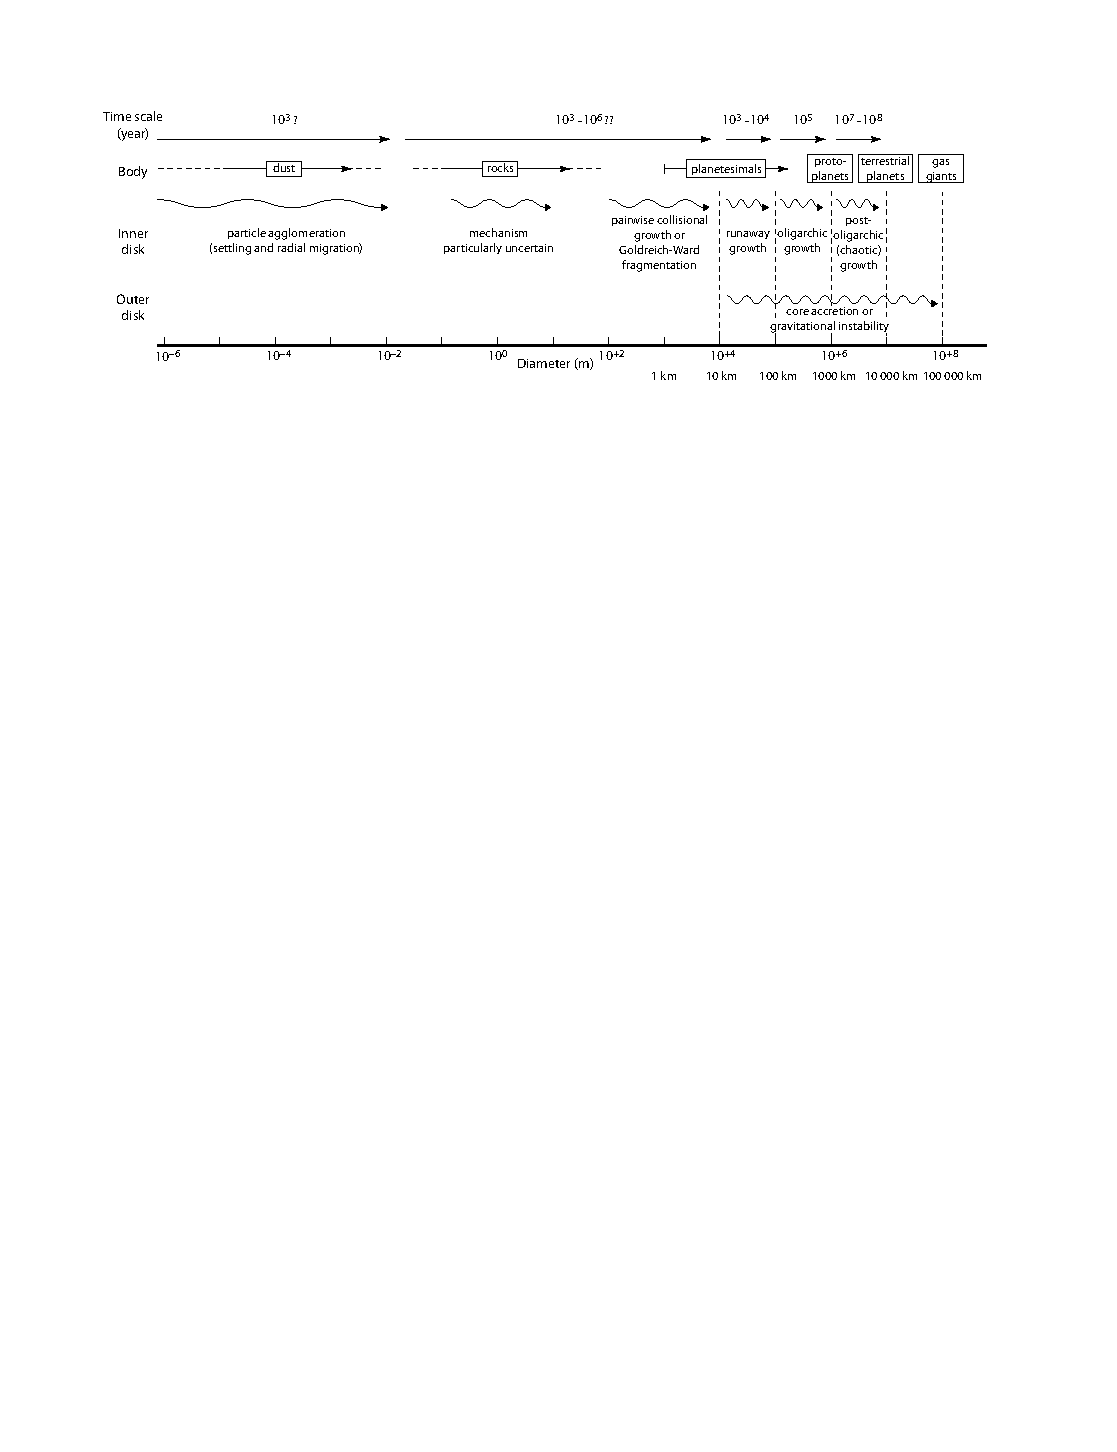
\includegraphics[width=1.0\textwidth]{figures/chapter1/fig11_pfsequence.pdf}
\caption[基于太阳系的传统行星形成理论模型在不同阶段的说明图,其中「米级障碍」属于至今为止的重大难题。图片版权 Michael Perryman。]{基于太阳系的传统行星形成理论模型在不同阶段的说明图,其中「米级障碍」属于至今为止的重大难题。此图取自文献 \citen{Perryman2014}。}
\label{fig:pfstage}
\end{figure}


\subsection{经典理论新挑战:系外行星} \label{sec: exopftheory}

由于观测极限,太阳系行星如今尚身处观测能力范围以外。如图\ref{fig:exomassper} 所示,
系外行星种类遍布多样,堪称「百花齐放」,且已确认数量仍在日趋增加。抛开观测选择
偏差(Observational Selection Bias),太阳系相比之下似乎显得有些「格格不入」。 按
照图\ref{fig:exomassper},本文将系外行星按照其集中区域大致分为三类: 热类木星族
(椭圆实线),冷类木星族(方框实线)和超级地球族(椭圆虚线)。

\begin{figure}[h]
\centering
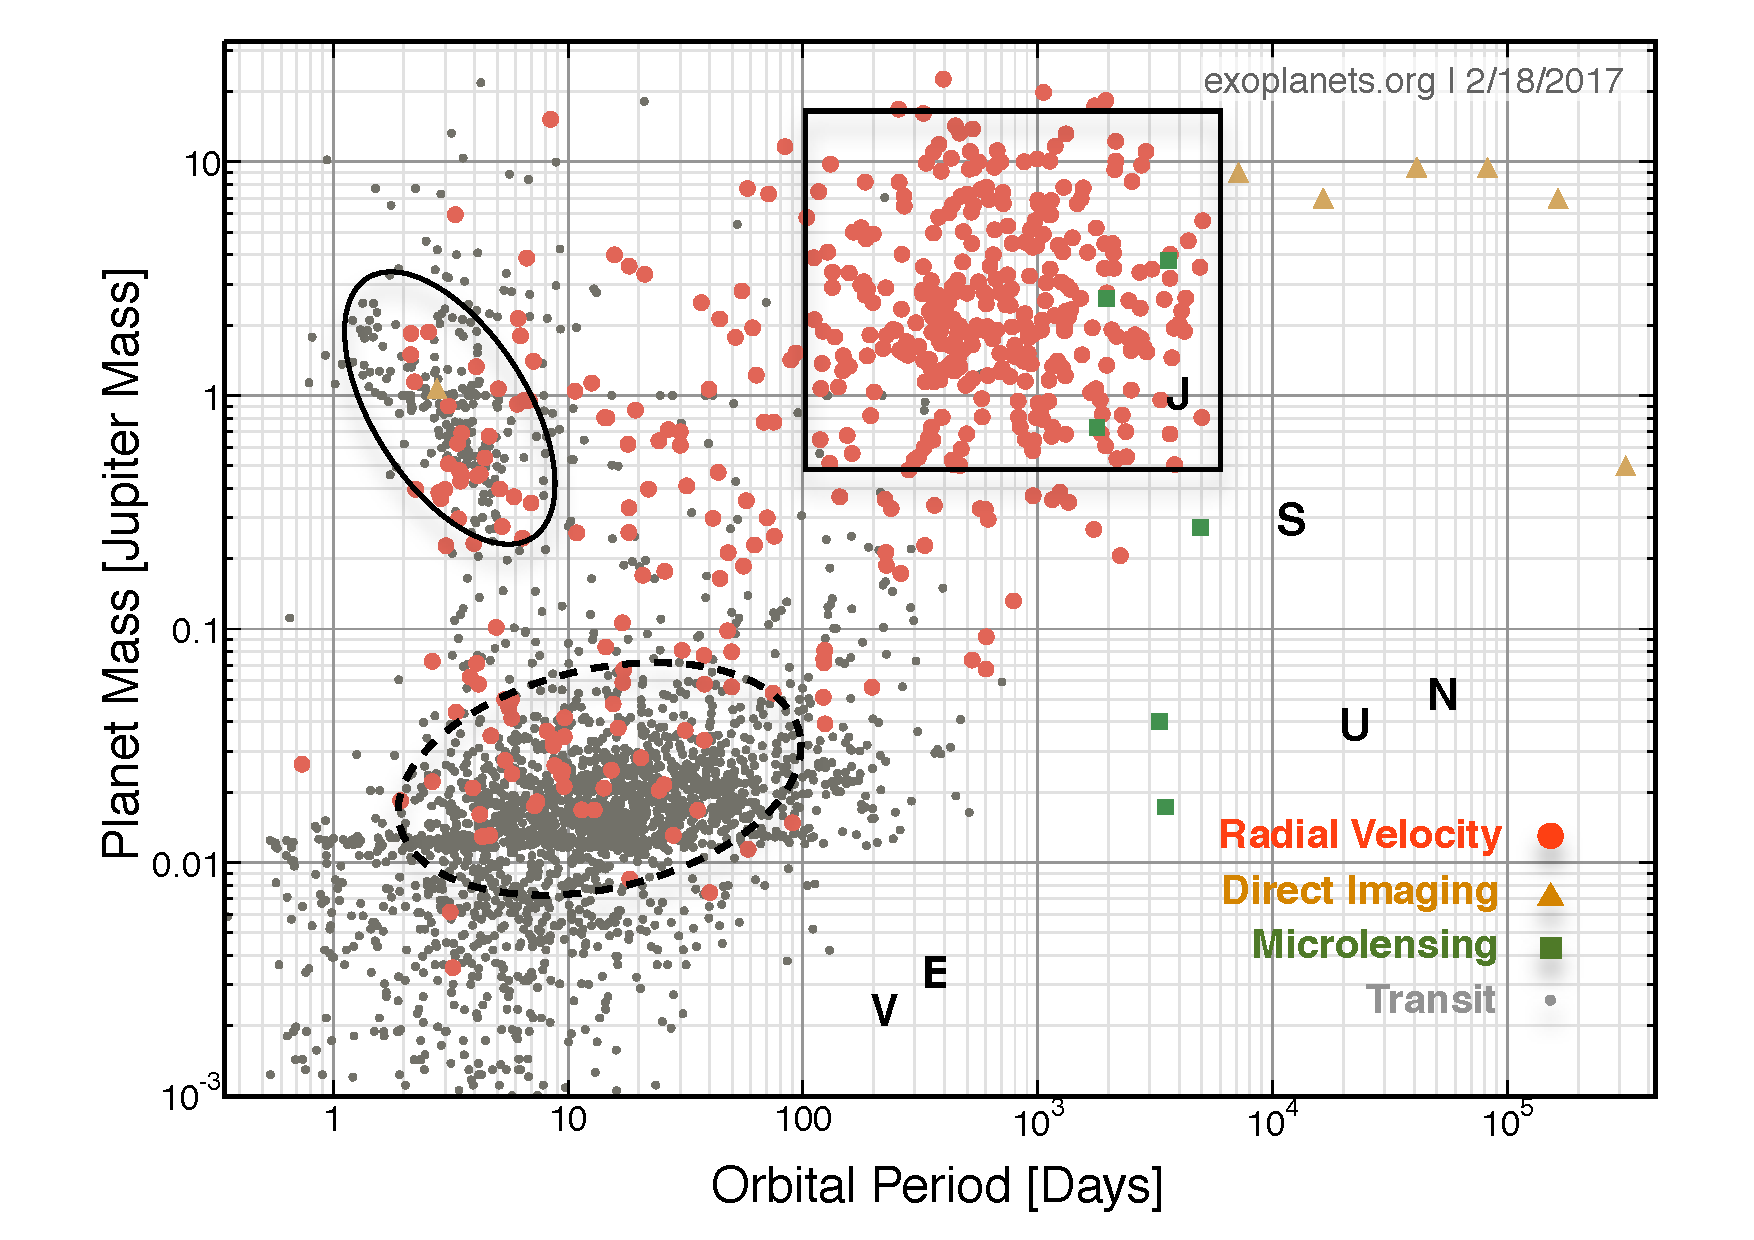
\includegraphics[width=1.0\textwidth]{figures/chapter1/fig12_nasaexompplot.pdf}
\caption{现今探测到系外行星的周期 --- 质量散点图。其中不同颜色分别代表不同的探测方法:红色代表视向速度法,灰色是凌星法,绿色指代微引力透镜法黄色代表直接成像法。黑色字母 V,E,J,S,U,N 则分别表示太阳系内金星,地球,木星,土星,天王星和海王星。本文将系外行星进行人为类别划分包络在封闭曲线内,分别为热类木星族(椭圆实线),冷类木星族(方框实线)和超级地球族(椭圆虚线)。此图取自 \url{http://exoplanets.org/}。}
\label{fig:exomassper}
\end{figure}

\subsubsection{热类木星族 Hot Jupiter Population}

当 Mayor 和 Queloz 与 1995 年发现第一颗围绕类太阳的系外行星 51 Peg b 时
\cite{MayorQueloz1995},整个行星学界都为之震惊,因为这颗类木星的轨道周期
只有 4.23 天。51 Peg b 单独用经典行星形成理论根本无法解释。由于此类行星非
常靠近其主星(轨道周期 $P \le10 $天),质量大于土星质量($0.3\,\tif{M}_\tif{J}$)故
而得名曰热类木星。作为本册论文重要的研究对象,此类行星详细的介绍内容请
参见 \S \ref{chapter:data_stat}。


\subsubsection{冷类木星族  Cold/Normal Jupiter Population}

与轨道距离主星较近的热类木星相对应有一类行星被称作冷类木星(或者常规类木星)。
此类行星在观测上拥有长于约一百天的轨道周期,有效温度也比热类木星低得多,太阳
系木星就属于一颗典型冷木星。相比短周期行星,确认此区域的行星通常需要望远镜
连续观测几年甚至数十年,因而样本完备性也相对较差\cite{Cumming2008}。根据使用
 Keck 望远镜进行的 Lick-Carnegie 行星搜索项目,Rowan 等人通过观测样本估算得到
此类行星的出现概率大概只有约 3\%(文献\citen{Rowan2016}),因而木星在人类想法
中先入为主、见惯非惯的概念也许并不周全。

另外值得提的一点是直接成像法(\S \ref{sec:drctimgmeth})可以观测到更长周期行星
,如 HR 8799 系统(文献\citen{Marois2008HR8799},详见图\ref{fig:hr8799})
等屈指可数的样本。传统的核吸积模型需要花很长时间来形成此类气巨星的胚胎核心。
相比之下,另辟蹊径的引力不稳定(Gravitational/Disk Instability,一般简称 GI )模型
\cite{Kuiper1951,Cameron1978,Boss1997}则可比较合理地解释这些巨行星是如何形于
距离主星几十个天文单位的轨道上\cite{Durisen2007}。



\subsubsection{超级地球族  Super-Earth Population}

超级地球,又称迷你海王星(mini-Neptune),对于 RV 探测到的系外行星一般定义为
介于十个地球质量与海王星质量之间。而对于凌星法探测到的行星,则其半径大约介于
二到四个地球半径\cite{Haghighipour2011}。在图\ref{fig:exomassper} 中,不难发现超级
地球十分常见与 1 天至 100 天之间的轨道,Batalha 等人利用 Kepler 前 16 个月的数据
也推断超级地球为银河系最常见的行星类别\cite{Batalha2013}。

那么超级地球的形成历史究竟何般?它们又是否可归至类地行星范畴呢?前面 \S 
\ref{sec:clspftheory} 提到在核吸积模型下,气态巨行星首先会成长为约 10 
$\tif{M}_\oplus$ 的固态核心后通过吸积气体而成长\cite{Guillot2005}。超级地球质量
也正好估算为此值附近\cite{Lissauer2011MRR},因而很自然的假设便是此类行星在
雪线之外形成并且轨道迁移至如今的位置\cite{Terquem2007,Kennedy2008,IdaLin2008}。
然而也有争论认为在 M 型矮星周围,超级地球完全可以于当地形成($in\:situ$ formation,
文献\citen{Laughlin2004,Kennedy2006,Hansen2013,Chiang2013,Boss2006})。
或许随着越来越多的超级地球内部结构被观测所限制后,此难题才可被解答\cite{Lissauer2014}。

另外,超级地球一般存在于多行星系统中\cite{Borucki2011},而且 Fabrycky 等人发现
这些行星倾向于聚集在平运动共振(Mean Motion Resonance,简称 MMR)的内边缘,
尤其是 3:2 和 2:1 平运动共振\cite{Fabrycky2014}。一时之间包括潮汐作用、共振结构
等解释众说纷纭\cite{LithwickWu2012,Lee2013,Batygin2013,Baruteau2013,Delisle2014,Chatterjee2015},
到如今也尚未弄清其中的动力学机制,还有此现象是否依赖于超级地球的形成过程。

\subsubsection{值得一提的行星系统} 
%https://en.wikipedia.org/wiki/List_of_exoplanet_firsts

除了以上三大类系外行星系统,本文额外汇总了一些有趣的行星系统(Planet of Interest),
它们诡怪的轨道构型在某种程度上令人叹为观止,甚至挑战了现有的行星形成理论。

\textbf{共振系统} --- \textit{GJ 876}  {} 2001 年,Marcy 等人发现 GJ 876 b 和 c 两颗类木行星周期比
接近 2:1\cite{Marcy2001}。几年后,Rivera 等人更是发现 GJ 876 的额外一颗行星 d 与前两颗
处于 Laplace MMR\cite{Rivera2010}。这和太阳系木星的内侧内伽利略卫星 Io,Europa 以及 
Ganymede 的构型堪称如出一辙。理论上,此类轨道构型很有可能是行星在气体盘中迁移所致
\cite{KleyNelson2012,ZhangZhou2010}。

\textbf{紧凑系统} --- \textit{Kepler-11}  {} 它因其 6 颗行星的紧密轨道构型\cite{Lissauer2011}而被称作太
阳系的孪生子系统\cite{Zhou2012}。行星在如此紧凑的系统几乎处于稳定的边缘\cite{Mahajan2014}。
此紧密构型起源也是一直处于争辩中,关于 Kepler-11 行星系统形成理论详见文献\citen{Angelo2016}。
此类系统还有另外一个有代表性的例子:HD 10180\cite{Lovis2011}。

\textbf{双星系统行星} --- \textit{$\gamma$ Cephei b}  {} ,双星系统中的行星分为卫星型与行星型
\footnote{卫星型又称 Satellite/Circumprimary Type,构型为行星围绕双星中的一颗运转;行星型
或称 Planet/Circumbinary Type,构型为行星轨道围绕双星的质心。},其中$\gamma$ Cephei
\cite{Hatzes2003} 系前者,而 Kepler-16\cite{Doyle2011} 则属后者。如图 \ref{fig:pibinary} ,近距离双
星中的行星系统与单恒星周围相差迥异,这是因为存在伴星的引力干扰,导致行星系统形成过程大相近
庭。关于此类行星系统,请详见书籍\citen{Haghighipour2010}。

\begin{figure}[h]
\centering
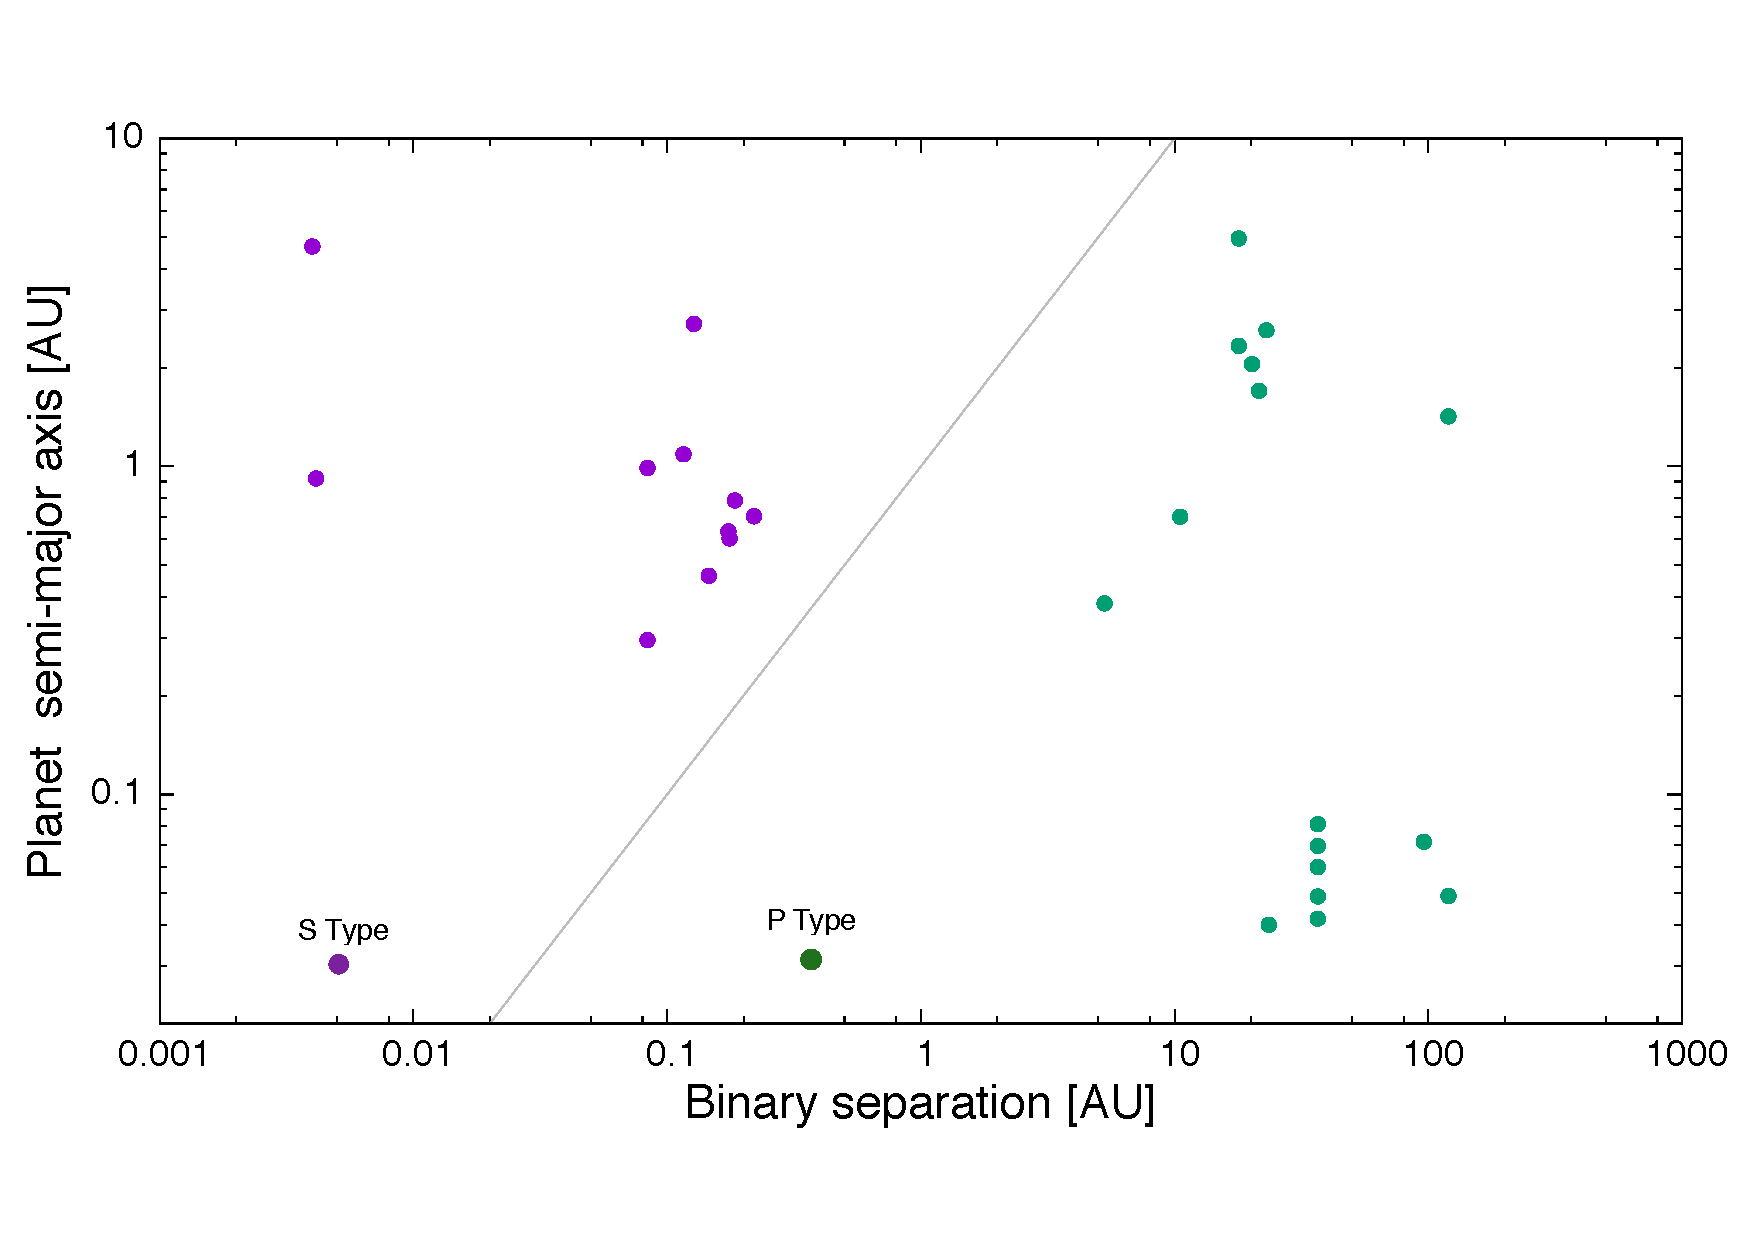
\includegraphics[width=1.0\textwidth]{figures/chapter1/fig13_binaryplanet.pdf}
\caption{已知双星内卫星型(S Type)与行星型(P Type)行星系统中双星和行星轨道半长径分布图,数据来自 \url{http://openexoplanetcatalogue.com}。}
\label{fig:pibinary}
\end{figure}

\textbf{高偏心率系统} --- \textit{HD 80606}  {}  作为偏心率最大的几个系统之一,HD 80606 拥有 0.93 的
轨道偏心率\cite{Naef2001},远心点居然是近心点距离的近三十倍。同属此类的系统还有 HD 4113
\cite{Tamuz2008},HD 80606 行星轨道法向和主星自转轴方向测量(Spin-Orbit Measurement )
\cite{Pont2009}表明它们的起源很可能与 Lidov-Kozai 机制\cite{Lidov1962,Kozai1962}有着密切关联
\cite{Wu2003}。

\textbf{极短周期行星} --- \textit{Kepler-78 b}  {}  极短周期行星又称(Ultra Short Period Planets, USPs),
它们因周期通常在一天以内,和主星表面的距离非常近而得称。代表性行星有 Kepler-78 b(周期为 
8.5 小时\cite{SanchisOjeda2013}),Kepler-70 b(周期仅 5.8 小时\cite{Charpinet2011})等。由于
它们受到主星强烈的辐射与引力作用,因而通常拥有非常大的密度,近年来也越发成为行星与主星物
理性质新实验基地\cite{Lopez2016,Moutou2016}。

\textbf{主序后恒星} --- \textit{HD 13189}\cite{Hatzes2005}  {}  虽然利用 RV 探测主序后恒星周围行星的效
率并不高\cite{Sato2005},但是此类行星依然对检验行星对恒星的质量、演化历史依赖度极为重要
\cite{Kennedy2008,Johnson2007b,Jones2014}。观测显示巨星周围的行星普遍距离主星较远
($a > 1\,\tif{AU}$),这也许正是主星演化吞噬近距轨道行星的证据\cite{Johnson2007a,Bowler2010}。

\begin{figure}[h]
\centering
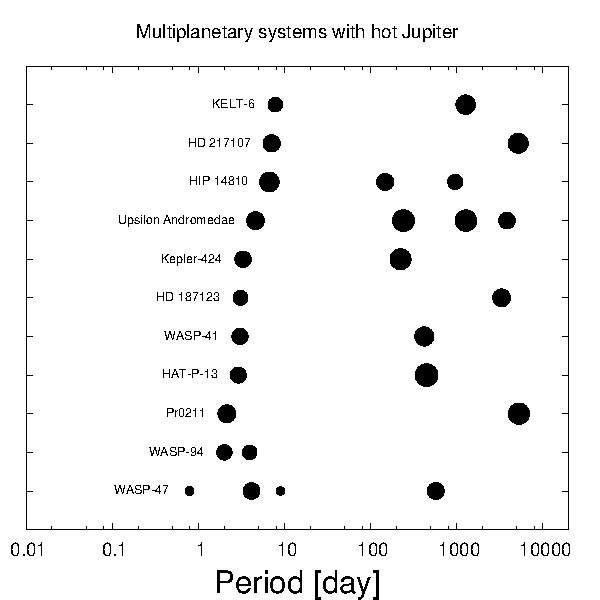
\includegraphics[width=1.0\textwidth]{figures/chapter1/fig14_hjmul.pdf}
\caption{所有拥有热类木星的已确认多行星系统汇总图,点的相对大小正比于行星的质量。数据同样来自 \url{http://openexoplanetcatalogue.com}。}
\label{fig:hjwcomp}
\end{figure}

\textbf{其他诡怪系统} --- \textit{WASP-47} {}  该行星系统拥有一颗典型的热类木星\cite{Hellier2012},
然而后续长期检测显示该系统有另外两颗小质量行星\cite{Becker2015,SanchisOjeda2015}以及一颗
长周期冷类木行星\cite{NeveuVanMalle2016}。这和传统的认为热类木星更倾向于成单的想法截然不同
\cite{Steffen2012},并且即使与其他包含热类木星的多行星系统相比,WASP-47 也大有不同(如图 
\ref{fig:hjwcomp}),现有的理论并不能完全解释该系统的构型,因而更完善的形成理论与观测限制
也更加迫在眉睫。

另外对疏散星团以及球状星团的巡天显示,Free-floating Planets(FFPs)也许是潜在的数量
最多的行星质量天体\cite{Lucas2000,Bihain2009,Sumi2011},星团环境作为系外(内)行星
的出生环境\cite{Adams2010,Liu2013} ,也不得不考虑该环境的反馈作用。


\section{本文立意}






%%%%%%%%%%%%%%%%%%%%%%%%%%%%%%%%%%%%%%%%%%%%%%%%%%%%%%%%%%%%%%%%%%%%%%%%%%%%%%%
\chapter{基于南极的天文数据观测与处理} \label{chapter:obs_red}

\section{南极天文背景} \label{sec:antarticabg}

搜索系外行星需要长时间基线和高精度的天文观测,然而因为地球在做周日自转并且存在大气包层,
因而在地球上很难同时满足这些严苛的观测条件。\S \ref{sec:transit} 中曾提到空间望远镜 CoRoT
\cite{Bargeetal2008CoRoT} 与 $Kepler$\cite{Boruckietal2010},它们花费了昂贵的代价(数十亿
美元)才能得到满足上述观测条件的数据,事实证明它们也取得了令人瞠目的科学成果。而横向对比,
南极台址(Antarctic plateau)作为理想的地面台址可在经费花费相对较少的同时,依然拥有良好的
观测条件 --- 而这得归功于以下几点优势:

\begin{enumerate}[leftmargin=1\parindent] 
\item[--] 南极高台地址拥有大陆上最冰冷、干燥\footnote{以绝对水气值来衡量。}的空气(文献\citen{Burton2010} )。此气候条件尤为适合进行光学、红外以及亚毫米波段的天文观测\cite{Lawrence2004}。
\item[--] 南极高台水平高度高,因而空气层厚度薄,大气湍流少,空气状况也更稳定\cite{Bonner2010}。
\item[--] 极夜(Polar nights)为观测提供了长达 3 个月的连续观测条件,这也是观测系外行星最重要的优势\cite{Rauer2008}。
\end{enumerate}

\begin{figure}[t]
\centering
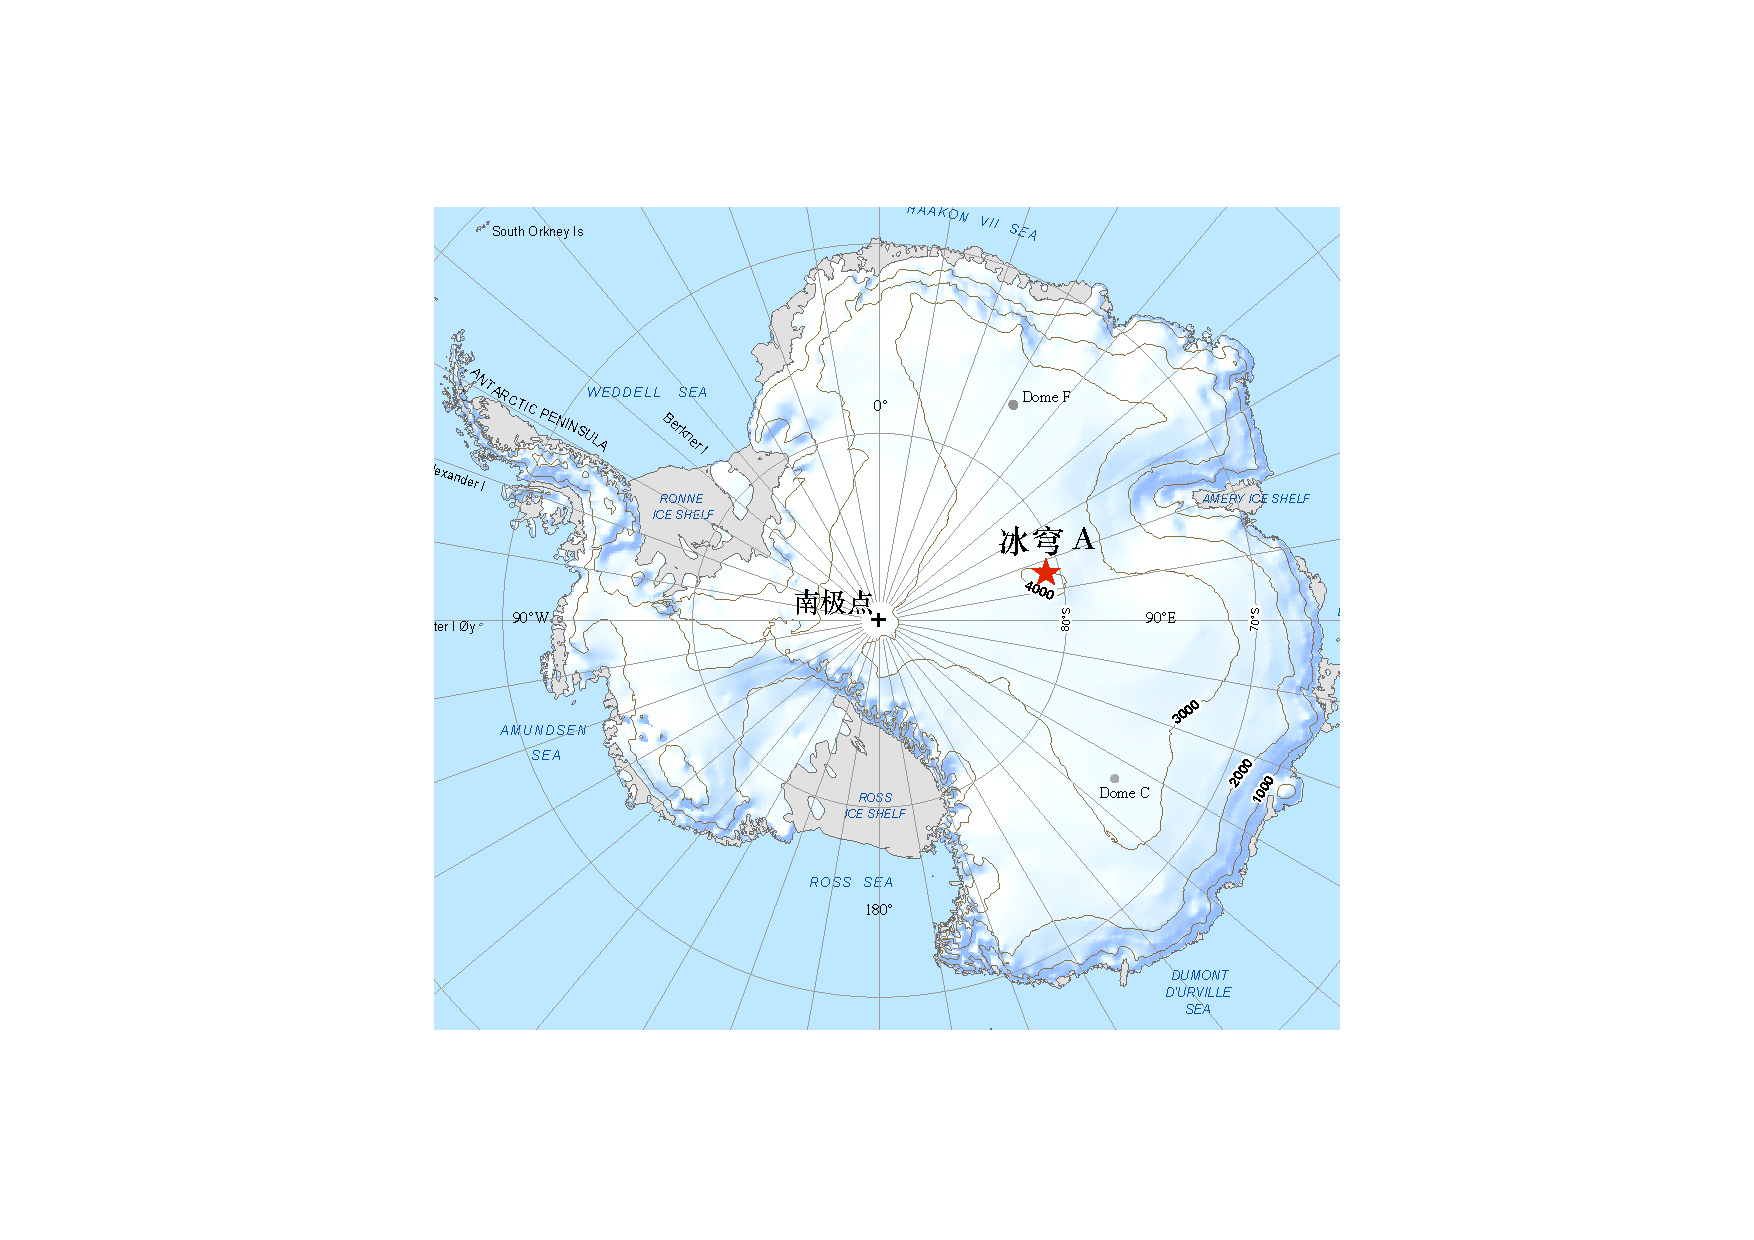
\includegraphics[width=1.0\textwidth]{figures/chapter2/f1_DomeA.pdf}
\caption{南极地理位置图,暗咖啡色曲线表示地形等高线。可以看到 Dome Argus(或称冰穹 A)台址(中国,以红星标注)位于南极大陆最高点,另外冰穹 C(澳洲) 和 F(日本)分别以灰色圆点表示。此地图版权 Australian Antarctic Division。}
\label{fig:domeasite}
\end{figure}

得益于拥有如此得天独厚的先天条件,南极台址在短短 30 年内就已吸引了大批的天文开拓实验与项目
(南极天文的历史相关细节请查阅综述文献\citen{Indermuehle2005})。Grec 等人于 1980 年开启首个
地处南极的光学实验\cite{Grec1980}。随后一大批天文学成果相继涌现\cite{Burton2010},以高精度测光
科学为例:ASTEP(Antarctic Search for Transiting Extrasolar Planets)项目先后于 Dome C 观测台址
捕捉到 WASP-19 b 次掩食的证据\cite{Abe2013STEP},并对该台址在凌星法探测系外行星领域的可行
性作出测试\cite{Crouzet2010}。

Dome A(位于昆仑站附近,坐标 $80^{\circ}37'S$ and $77^{\circ}53'E$,如图 \ref{fig:domeasite})作为
南极大陆最高的台址(海拔高度 4093m)在南极天文领域有着特殊的地位。Saunders 在比较过云层覆
盖率、空气对流层厚度和视宁度(seeing)后,指出 Dome A 也许是地面潜在的最佳天文观测台址(文
献\citen{Saunders2009})。中国南极天文中心也于 2008 年成功将中国之星小望远镜阵(Chinese 
SmallTelescope ARray,简称 CSTAR)成功安装就位于冰穹 A 台址。在极地冰寒的环境下需要克服许多
的障碍\footnote{关于南极天文科考支撑平台,请参见网址 \url{http://www.ccaa.pmo.cas.cn/njtwt/201312/t20131203_144501.html}。},
CSTAR 也取得硕果累累的成果,本文将于 \S \ref{sec:cstar} 中详细介绍如何通过修正鬼像(ghost 
image)来提高数据精度。另外 \S \ref{sec:ast3} 将简单描述 AST3(Antarctic Survey Telescopes)巡天
项目中系外行星搜寻计划的观测策略。


\section{CSTAR 以及其测光数据中的鬼像处理}  \label{sec:cstar}
\subsection{CSTAR 望远镜光学设计和预数据处理}  \label{sec:cstardesign}
作为 PLATO 平台\cite{Lawrence2009,Yang2009}下一台子设备,CSTAR 望远镜由南京天文光学技术研
究所(Nanjing Institute of Astronomical Optics \& Technology,即 NIAOT)承担设计工作。CSTAR 阵
列由 $2\times2$ 共四面施密特卡式(Schmidt-Cassegrain)望远镜组成,每面镜子大小 145 mm 口径:
其中三面拥有与斯隆数字化巡天类似的 $g,\,r,\,i$  宽带滤镜,另一面无滤镜。望远镜在设计上被固定于地
表,因而观测模式为指向天顶附近的南天极天区保持凝视,考虑此做法也是因为这样更有利于研究天文
变源。CSTAR 成像后端匹配了 Andor DV435 型号 1k$\times1k$ 的 CCD,联合望远镜 $4.5^\circ{} 
\times 4.5^\circ{}$ (20 deg$^2$) 的视场(Field Of View 或 FOV)大小,可知一个像素(pixel)对应于
天球 15$''$ 的张角\cite{Yuan2008}。图 \ref{fig:cstaroptics} 展示的是 CSTAR 内部光路结构,在已有的 
$i$ 波段数据中,入射镜的表面覆盖了滤光片,且子镜(中间镜)也涂有反射膜,恒星的光线容易在两面
涂层之间反射,从而导致鬼像的产生。

\begin{figure}[t]
\centering
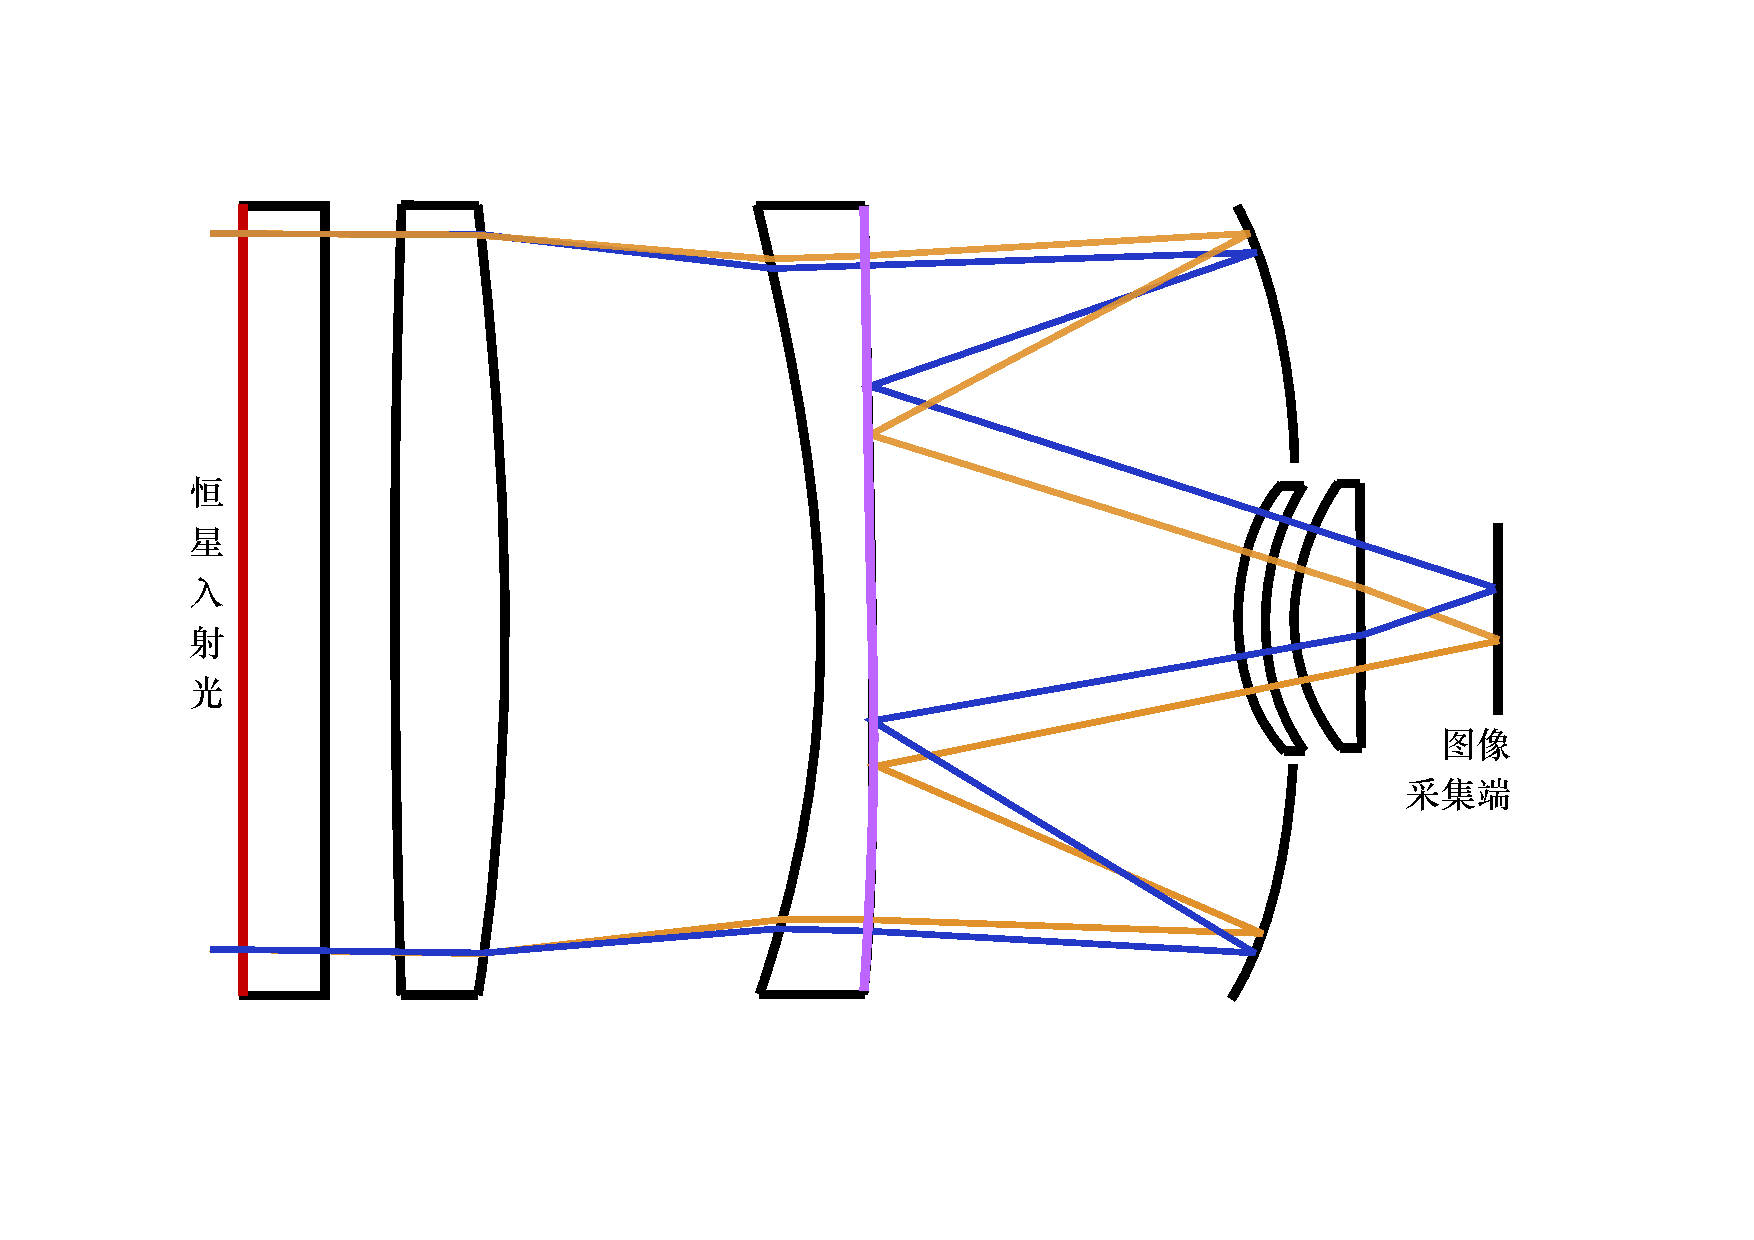
\includegraphics[width=1.0\textwidth]{figures/chapter2/f2_cstaroptics.pdf}
\caption[CSTAR 多镜面结构光路设计图。入射平板镜(最左侧)由改正镜与滤镜组成,最右侧的镜片为中空反射球面镜,中间子镜的右侧面涂有反射材料,该图与实际大小不成比例。]{CSTAR 多镜面结构光路设计图。入射平板镜(最左侧)由改正镜与滤镜组成,最右侧的镜片为中空反射球面镜,中间子镜的右侧面涂有反射材料。作图时未按照实际比例,参考自文献 \citen{ZhouX2010a}。}
\label{fig:cstaroptics}
\end{figure}

CSTAR 于 2008 年 1 月份,正式跟随南极科考队抵达冰穹 A 站点,可惜的是在第一个观测季度结束后,
望远镜只剩下 $i$ 波段镜面能正常观测。于是从 2008 年 3 月 4 日至 8 月 8 日(冰穹 A 站极夜),
CSTAR 共以 20 秒或 30 秒的曝光时间拍摄了超过 310,000 张图片。多亏了极夜创造的连续不间断观测
条件,这些总曝光时间长达 1,728 小时的图片数据表现出良好的科学状况与条件。

随着极昼的到来,科考人员取回了 CSTAR 的原始观测数据,国内两个小组分别开始了独立的分析工
作,国家天文台南极天文小组于 2010 年分别计算了台址当地 $i$ 波段的天光背景以及大气透明度
\cite{Zou2010},并释放出超过 10,000 颗恒星点源星表\cite{ZhouX2010b}。Wang 等人\cite{Wang2011}
则于来年在光变数据中找出了 157 颗变星(这高于该天区先前所知数量 6 倍)。随后 Wang 分别在随后
分别对测光给出大气消光、不均匀云层和周天效应的修正(文献 \citen{Wang2012,Wang2014})。

下面,本文将简要介绍文献 \cite{ZhouX2010b} 的主要数据处理流程。在完成扣除本底和平场等预数据
处理后,Zhou 对每张原始图片采用了以 3,4 和 5 为半径的孔径测光(apeture photometry)。接着,
一张测光条件较好的图被选用作为标准参考,并用模式匹配来认证不同图内相同参考星的位置变化,并
同时矫正其他图片内点源的星等偏差量。以上操作得到标准星表后,其中 48 颗恒星被挑选出来和 
USNO-B1.0 参考星表对比从而得到最终星表。在以上的工作中,作者发现数据中的鬼像修正对于进一步
提高测光精度有着非常重要的意义。

\subsection{鬼像简介以及修正 CSTAR 数据中的鬼像} \label{sec:ghost}

\subsubsection{鬼像以及 CSTAR 中的鬼像}
正如前文(\S \ref{sec:cstardesign})提到,鬼像在光学系统中并不算罕见,尤其是拥有大视场的施密
特望远镜。U.K. 施密特望远镜单元(UKSTU) 将鬼像的产生原因共归为五类,分别是乳化剂涂层、滤
片修正镜、改正镜、滤光片以及尖状鬼像。CSTAR 在设计上采取施密特卡式光学设计,因而鬼像很可
能产生于恒星入射光传播、折射与反射的过程中。UKSTU 手册\cite{1983ukstu} 将此类鬼像定性形容成
弥散状的斑点,且鬼像光斑坐标与产生鬼像的亮源位置关于光学轴对称。对于 CSTAR 而言,鬼像修正
十分必要,因为鬼像不仅会被误认证成一颗恒星源,还会叠加在背景恒星上从而造成额外的测光误差。

\begin{figure}[t]
\centering
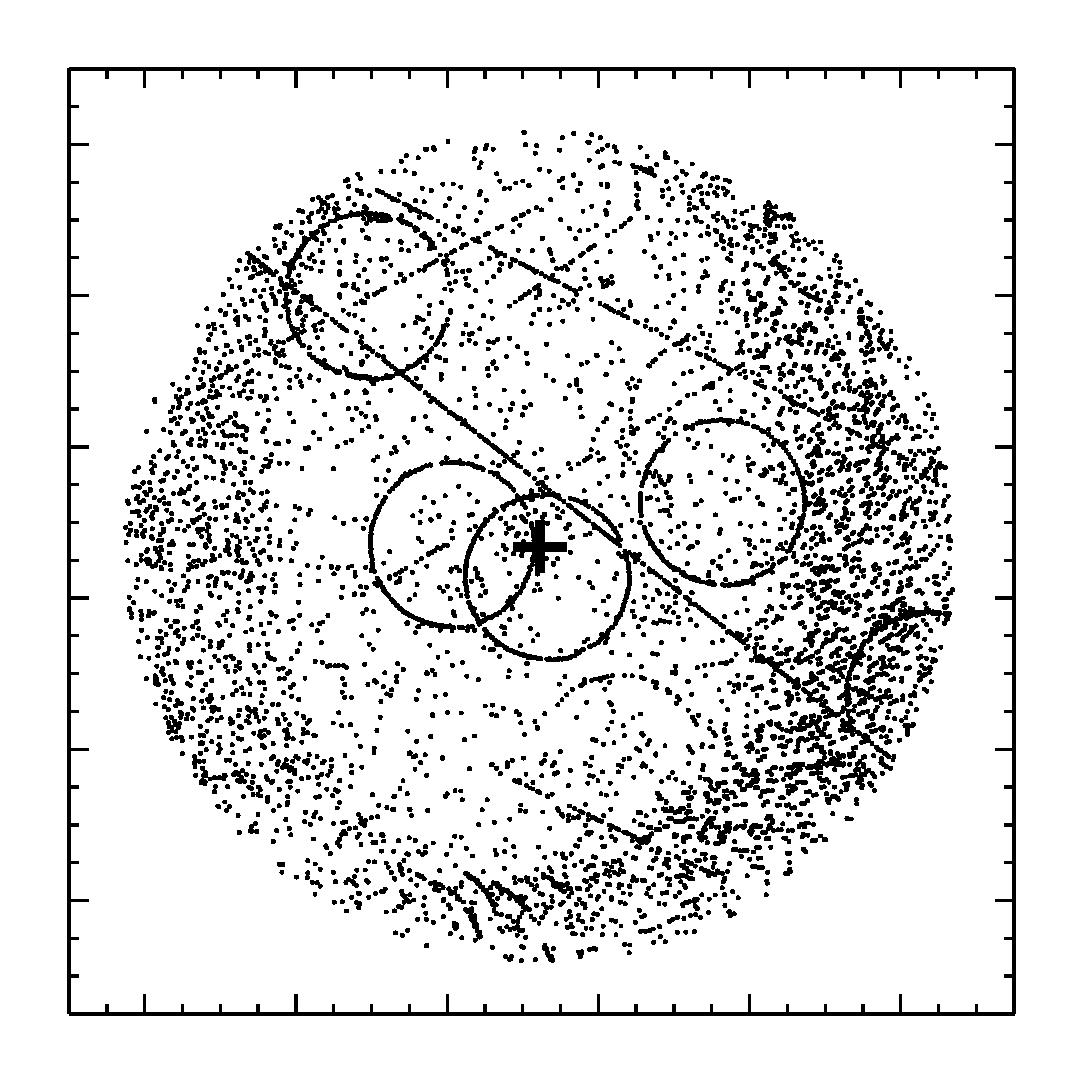
\includegraphics[width=1.0\textwidth]{figures/chapter2/f3_ghoststack.eps}
\caption{周天鬼像叠加图,也即「脏」图。图中的圆弧结构为鬼像所致,黑色十字标注的是南极点。为了更好的看清鬼像的结构,我们已经将已确认的恒星从本图中剔除,此外图中线状物为人造卫星。}
\label{fig:ghoststack}
\end{figure}

作为第一代南极天文望远镜,CSTAR 采取相对安全的凝视模式 --- 望远镜支撑点固定在冰层上,并
且对准南天极附近的天区观测。当恒星做周日运动时,星象斑也会在 CCD 上绕着南极点做近圆周运
动。若选取图「A5CH5029」作为标准参考图,那么经过恒星图案模式匹配(pattern match)后,其余
所有图相对于标准参考图的旋转角度便可被计算出。从而不同时间测得的图像内相同位置的恒星可被识
别认证。此时将相同恒星的本地坐标(pixel coordinate)通过旋转缩放等操作转化成标准参考图内的坐
标后,便可得到与其对应的主坐标(master coordinate)。从上一段文字中,已经得知鬼像(假恒星)
与产生鬼像的亮星关于光学轴对称,所以当恒星们时时刻刻被匹配上的同时,鬼像却只能经过一个周天
后才能匹配上自己。若把一天之内所有拍摄的图片作叠加,然后将同一颗恒星给抹去后,我们可得到周
天鬼像叠加图(请查阅图 \ref{fig:ghoststack})。从图中可以看出,鬼像的转动方向与周日运动方向相
反,鬼像因此也很可能周期性地「撞」到恒星。当然,如果将南极冰川板块的微弱移动\cite{ZhouX2013}
与恒星自身的运动考虑在内,鬼像很有可能在一天内遭遇到多颗恒星,从而对恒星亮度造成多达约 1.0 
星等的变化(如图 \ref{fig:lcwghost} 与 \ref{fig:ghostseq})。若不小心处理这种变化很可能会被误认为恒
星自身的性质,例如恒星耀斑\cite{Liang2016},因此修正鬼像是后续天体物理研究(如搜寻系外行星
\cite{Wang2014CSTAR} 以及变星\cite{Yang2015}等)的基础工作。

\begin{figure}[t]
\centering
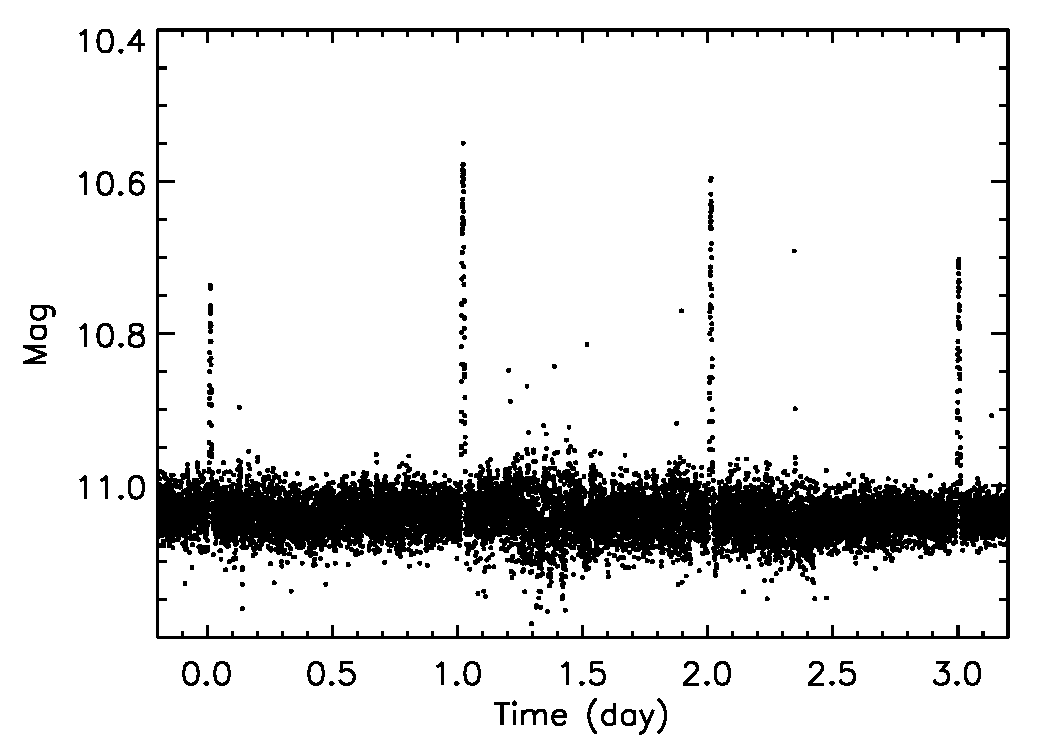
\includegraphics[width=1.0\textwidth, trim={0.0cm 0.5cm 0 0}]{figures/chapter2/f4_lcwghost.eps}
\caption{CSTAR 视场内坐标为 R.A.: $23^\tif{h}24^\tif{m}28.4^\tif{s}$,decl.: $-89^{\circ}25'10.6''$ 的恒星的光变曲线。通常此特定鬼像会在一个恒星日内遭遇该被影响的恒星一次,从而将恒星的亮度提高半个星等。}
\label{fig:lcwghost}
\end{figure}

\begin{sidewaysfigure}
\centering
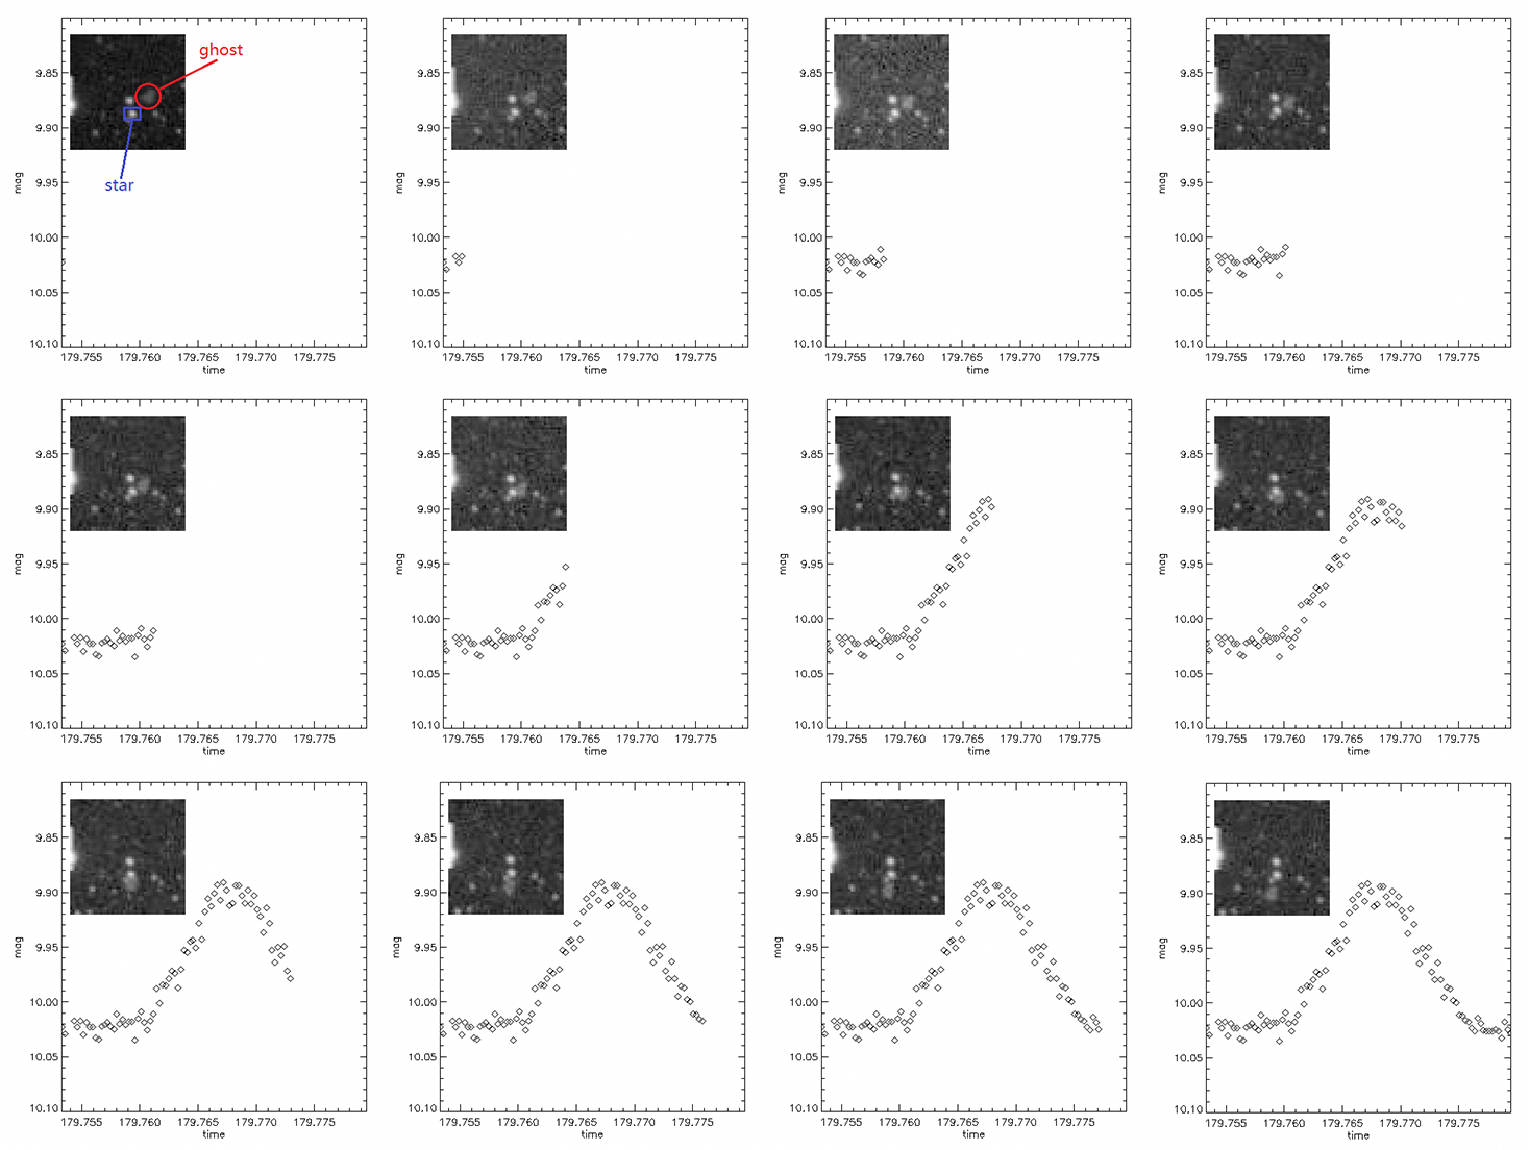
\includegraphics[scale=0.8]{figures/chapter2/f5_ghostseq.pdf}
\caption[坐标相对固定的恒星(蓝色标志)遇到鬼像(红色标注的模糊状弥散源)前后恒星星等的变化程度原始图片数据示意。]{坐标相对固定的恒星(蓝色标志)遇到鬼像(红色标注的模糊状弥散源)前后恒星星等的变化程度原始图片数据示意。每张快照的纵坐标为星等值横坐标为时间,如需查看此图清晰的动画版本请前往网址 \url{https://github.com/meldonization/PhD_Dissertation/blob/master/figures/chapter2/ghost_animation.gif}。}
\label{fig:ghostseq}
\end{sidewaysfigure}


\subsubsection{CSTAR 鬼像修正方法}

为了扣除所影响的恒星的流量中鬼像的污染,我们首先得确认产生这些鬼像的前身,即视场中的亮源。
之所以采取此途径是因为鬼像通常为暗弱的延展源,背景噪声对它们的孔径测光影响很大,直接扣除
被影响恒星中鬼像的孔径测光流量的做法会非常不可靠。找到产生鬼像的亮源后,我们会将被被影响
恒星的星等变化程度极短出来,最后就可以对 CSTAR 的数据进行系统性的修正。

我们因此发展了一整套处理识别鬼像、计算并消除鬼像对恒星星等的影响的流程。具体如下:

\begin{enumerate}[leftmargin=1\parindent]

\item \textbf{确定光学系统对称轴和产生鬼像的亮源。} CSTAR 视场较大,点源密集,因而对每个鬼像
每张图做修正几乎是不可能完成的任务,这里我们只查找星场中最显著的鬼像环。由于望远镜观测的极
限星等限制,因而只有最亮的恒星才会产生鬼像。当我们将星表中的前 100 颗亮星与最明显的鬼像环圆心做匹配,那么匹配成功的亮星就是产生鬼像的源。一旦产生鬼像的源被确定后,我们便可将鬼像的主坐标 [$X$, $Y$] 转换成每张图片中的本地坐标 [$x$, $y$]。通过交叉联立此本地坐标和上文提到的亮星坐标,可以进一步得到望远镜系统的光学对称轴在 CCD 上的像素坐标值。

\item \textbf{定量的描述鬼像对背景星的影响。} 当知晓系统的光学对称轴后,我们可以从文献 
\citen{Wang2012} 中找到产生鬼像的恒星、鬼像以及被鬼像影响恒星的星等数值,且最后一个物理量
会随着鬼像和恒星之间的距离变化而发生改变。下文统一用 $d$ 替代鬼像中心与被鬼像影响恒星中心之
间的距离,用 $m_\tif{g},\,m_\tif{gs},\,m_\tif{s}^0$ 和 $m_\tif{s}^1$ 分别表示鬼像的星等、鬼像源亮星的
星等、被鬼像影响前后背景星的星等。本文采取两个基本假设:1. 鬼像源亮星流量与鬼像流量的转化率
为 $f_0$,即 $F_{\rm{g}}=f_0\cdot F_{\rm{gs}}$;2. 鬼像对背景星造成的光子数影响比例 $f_1 $ 只是
距离 $d$ 的函数,$\Delta F_{\tif{s}}=F_{\tif{s}}^1-F_{\tif{s}}^0=f_1(d)\cdot F_{\tif{g}}$。若此时带入流量与星等之间的转换关系 $m=-2.5\lg F+m_0$,我们可以得到如下两个等式:


\begin{equation} \label{eq:ghostformular}
\arraycolsep=1.4pt\def\arraystretch{2.2}
\left\{
\begin{array}{l}
m_{\tif{g}} = -2.5 \lg f_0 + m_{\tif{gs}} \\
f_1(d) \cdot f_0 \cdot C^{m_{\tif{gs}}} = C^{m^1_{\tif{s}}}-C^{m^0_{\tif{s}}}  \, \ ,
\end{array} 
\right. 
\end{equation} \myequation{修正鬼像星等差的基本公式}
其中常数 $C=\lg 2.5$。从统计上,我们可从鬼像、源恒星以及被影响的背景星的列表中拟合两个自由参
数 $f_0$ 和 $f_1(d)$。这里需要指出的是不同亮星产生的鬼像之间的参数并不完全一致,为了方便起
见,我们归一化处理了第二个参数 $f_1(d)$。

\item \textbf{修正星表中的鬼像影响。} 以上两步完成后,我们可估算每张图内的未知参数 $f_0$ 和 $f_1(d)$。假设图片拍摄时间为 $t$,那么在带入每张图内每个恒星的修正量后,可得到去除鬼像污染的新光变曲线序列 $(t, d, mag_{\tif{s}}, mag_{\tif{gs}})$以及全新的星表。

\end{enumerate}

\begin{table}[ht]
\centering
\caption{CSTAR 星表中主要产生鬼像的亮星列表。} 
\label{tbl:ghostsource}
\begin{tabular}{cccccc}%{1.0\linewidth}{@{\extracolsep{\fill}}ccccccc}
\hline \hline
CSTAR ID	&    R.A.   &   Decl.  	       &    masterX    &   masterY    &    $i$          \\ 
	        	&  (h:m:s) & (d:m:s) 	       &      (pixel)      &     (pixel)      &  (mag)       \\ \hline
00003   	& 49:03.3 & -88:16:34.99 & 7497.2864   & 1386.2566   & 6.1357  	\\
00004   	& 15:58.6 & -87:33:53.25 & 1350.1814   & 8661.678     & 6.1444  	\\
00006   	& 34:34.0 & -89:46:18.97 & 5129.6065   & 5103.6644   & 6.3055  	\\
00007  	& 08:26.2 & -88:57:34.07 & 2812.204     & 4118.1307   & 6.3671  	\\
00008   	& 15:55.2 & -87:58:09.94 & 1740.2338   & 1388.6649   & 6.4489  	\\
00009   	& 42:07.6 & -89:27:37.16 & 6386.3986   & 4679.7432   & 6.4995  	\\
00011  	& 20:07.4 & -88:14:48.27 & 8033.5867   & 7374.1179   & 6.5395  	\\
00012  	& 39:55.7 & -88:39:19.55 & 4151.218     & 7494.304     & 6.5944  	\\
00018  	& 45:45.4 & -88:48:57.98 & 2940.9191   & 3000.1653   & 6.8181  	\\
\hline \hline
\end{tabular}
\end{table}

\subsubsection{鬼像修正结果及讨论}

当拟合鬼像环半径数值(约 107 像素大小)、圆心位置坐标,并通过 match 程序
\footnote{源代码链接 \url{http://spiff.rit.edu/match/}}和文献 \citen{Wang2012} 给出的参考新表对比后,
我们得到了一批产生鬼像的恒星列表(表格 \ref{tbl:ghostsource})。由图 \ref{fig:starwghost} 可知鬼像
与源恒星 $i$ 波段的星等差约为 5.5,考虑到 CSTAR $i$ 波段的极限星等约为 14 等,因而在接下来计算
背景恒星星等受影响量的过程中,我们仅需考虑 $i < 8.5$ 的亮星产生的鬼像。

\begin{figure}[h!]
\centering
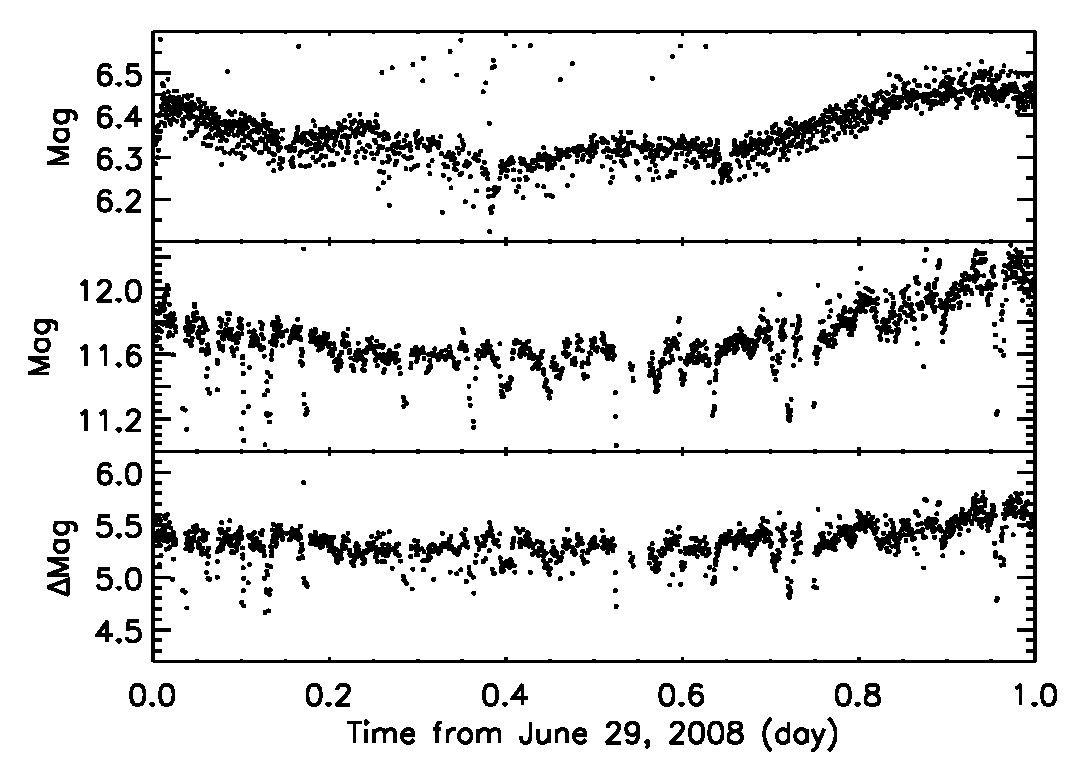
\includegraphics[width=0.92\textwidth, trim={0.3cm 0.5cm 0 0}]{figures/chapter2/f6_starwghost.eps}
\caption{上栏为产生鬼像的源恒星(R.A.: $21^\tif{h}08^\tif{m}44.2^\tif{s}$,decl.: $-88^{\circ}57'21.6''$)在一天内的星等变化图;中间栏为该源对应鬼像在这天内的星等变化;下栏为两者星等的差量。}
\label{fig:starwghost}
\end{figure}

\begin{figure}[h!]
\centering
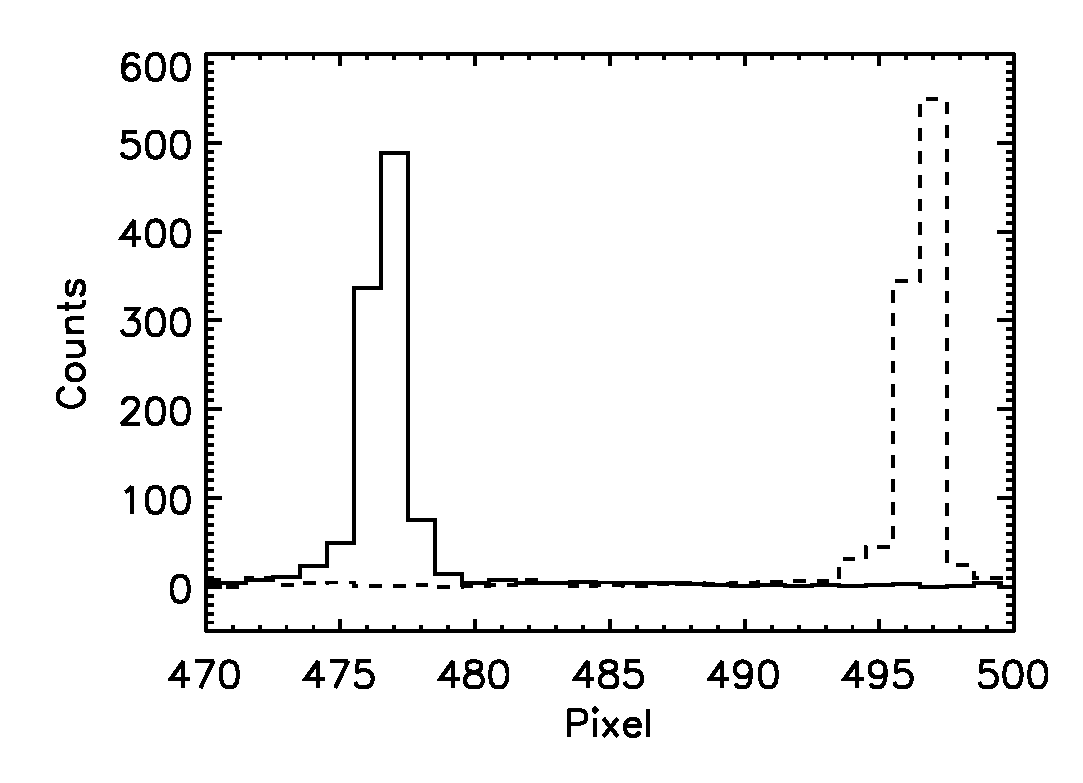
\includegraphics[width=0.92\textwidth,trim={0.5cm 0.5cm 0 0}]{figures/chapter2/f7_opticaxispix.eps}
\caption{光学对称轴在 CCD 上像素坐标的统计直方图,直方图格点宽度为一个像素点。图中实线为本地 $x$ 坐标像素值,虚线则为 $y$ 坐标。}
\label{fig:opticaxispix}
\end{figure}

然而在实际情况中,并不是所有星等量过 8.5 的恒星均会产生鬼像。亮星产生鬼像有很多条件,最重要
的两个因素是这些亮源距离视场中心以及光学对称轴的距离。原理上讲,当亮星距离视场中心或者对称
轴中心太远,它在镜面反射层之间被反射的光需要经过更长的光学路径来传播,产生的鬼像也因此而更
暗弱。


\begin{figure}[t]
\centering
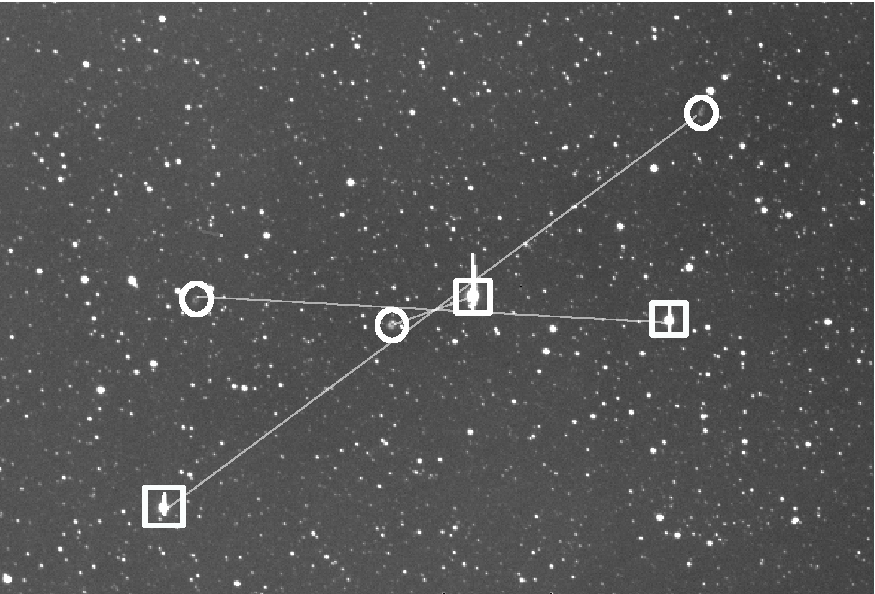
\includegraphics[width=0.95\textwidth]{figures/chapter2/f8_opticaxisimg.eps}
\caption{选定的图片文件名为「16RE0312.fit」的光学对称轴示意图。方框选中的亮源(垂直溢出条纹)与圆环内的弥散鬼像相交于同一个像素点,即光学对称点。}
\label{fig:opticaxisimg}
\end{figure}

在得到鬼像源亮星列表后,我们将该列表和鬼像环内的所有恒星做比较。这样做可以得到每张图中真正
的鬼像和 CSTAR 系统的光学对称轴在 CCD 上的像素坐标。如图 \ref{fig:opticaxispix} 所示,光学对称
轴的本地坐标为 $[477\pm2,\ 297\pm2]$。该值也同样经过真实图像的测试(图 \ref{fig:opticaxisimg})。
考虑到鬼像以及其对应产生亮源之间的几何构造,不难得到鬼像环半径与光学对称轴和南极点之间距离
的关系式:
\begin{equation} \label{eq:ghostgeometry}
r_{\tif{ghost}}=2\cdot d_{\tif{Pole, axis}} \ \ . 
\end{equation} \myequation{鬼像半径与南极点以及光学对称轴之间的几何关系}

如果将南极点的本地坐标值($[523,\,467]$)与上文提到的光学对称轴坐标值($[477,\ 497]$)带入上式,可算得鬼像的半径理论值为 109 像素,这和前面的拟合值一致。

\begin{figure}[ht!]
\centering
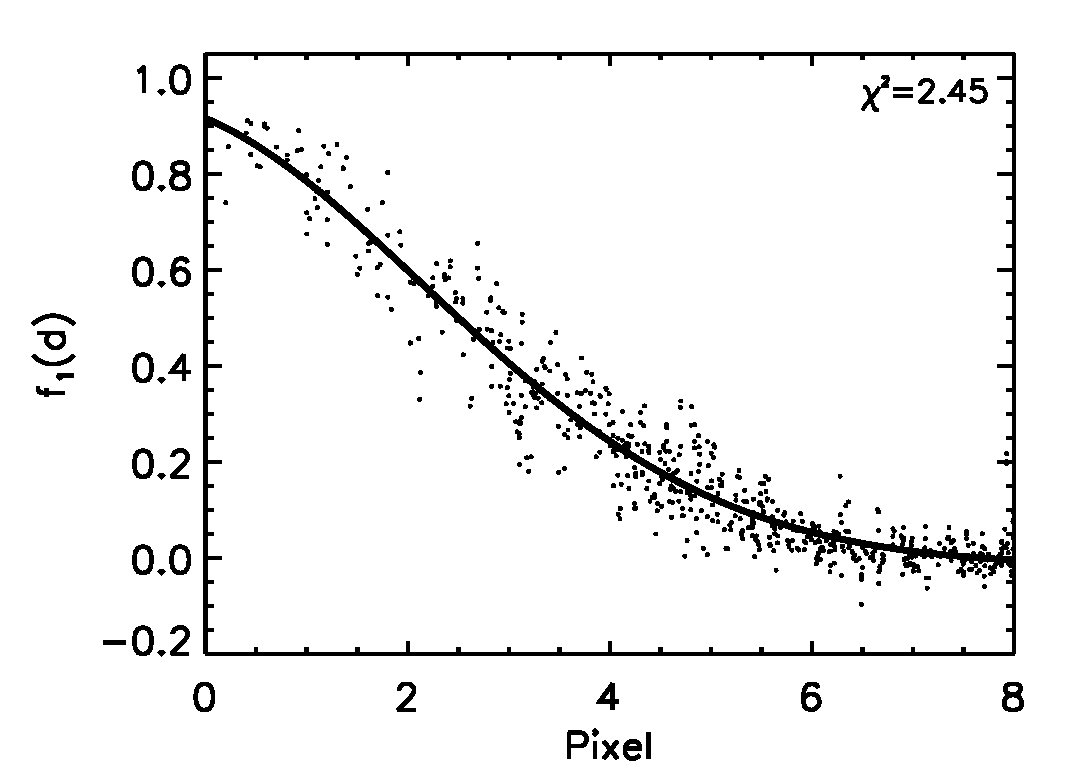
\includegraphics[width=0.8\textwidth, trim={0.5cm 0.3cm 0.5cm 0}]{figures/chapter2/f9_ghostfit.eps}
\caption{鬼像影响因子 $f_1(d)$ 与被影响背景恒星和鬼像之间距离的依赖关系。实线为形式如方程 \ref{eq:ghostf1d} 的拟合曲线,当两者之间的距离大于约 6 个像素时,鬼像几乎不对该星的亮度造成影响。相反,当鬼像完全重叠在背景恒星上时,鬼像自身高达 97\% 的光子流量都会被算入恒星的孔径测光亮度中。}
\label{fig:ghostfit}
\end{figure}

\begin{figure}[ht!]
\centering
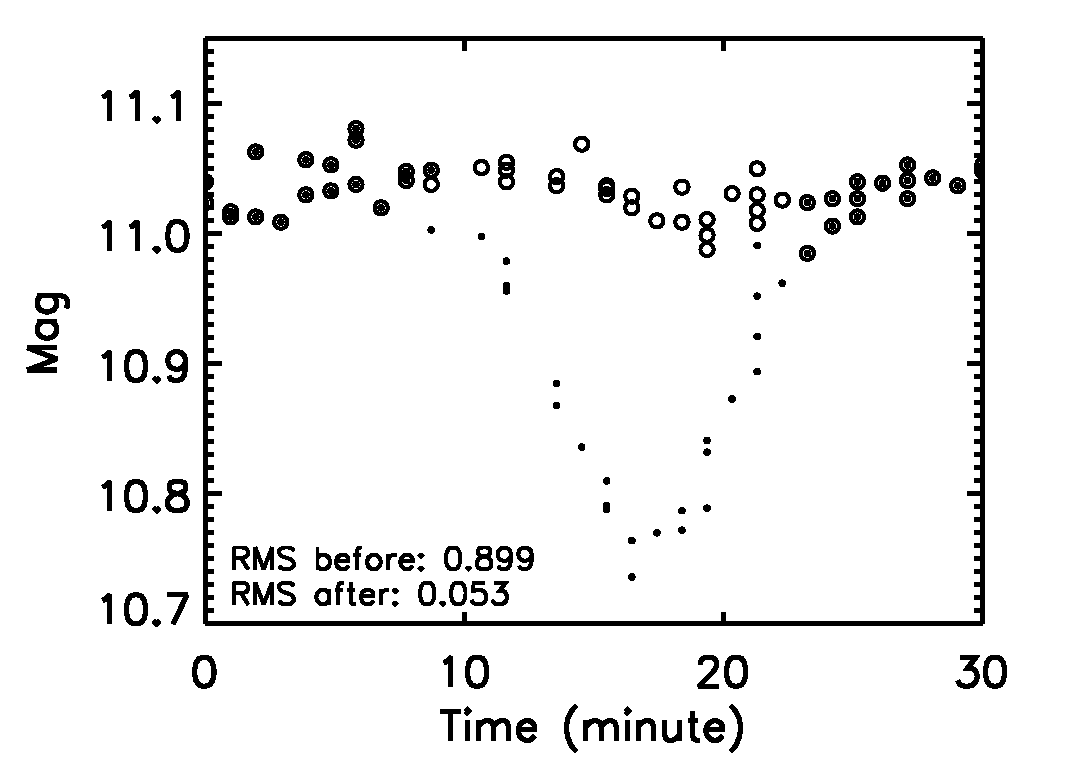
\includegraphics[width=0.8\textwidth, trim={0.5cm 0.3cm 0.5cm 0}]{figures/chapter2/f10_deghost.eps}
\caption{鬼像修正前后(分别为点和圆)恒星的光变曲线。此恒星坐标为 R.A.: $23^\tif{h}24^\tif{m}28.4^\tif{s}$,decl.: $-89^{\circ}25'10.6''$。当鬼像距离恒星达到 6 个像素点的临界值后,鬼像修正程序便会自动在恒星的光变曲线基础上计算影响值并做修正。如图所示,此方法可以大幅度减小恒星光变曲线的弥散误差。}
\label{fig:deghost}
\end{figure}


至于第一个影响因子 $f_0$,图 \ref{fig:starwghost} 已经展示了鬼像与亮星之间的亮度变化基本趋于一
致,这个差别值大概为 5.4 星等,即对应亮星 0.7\% 的光子流量被反射再聚集成鬼像。但与此同时,
我们应该意识到实际中的鬼像更加复杂:不同的位置、星等都会给 $f_0$ 因子带来不确定性。

如此一来,在计算第二影响因子的过程中,我们一律假设 $f_0 =  0.7\% $。在对星象班等天文观测数据中,很自然便是假设此函数为高斯函数。因为鬼像与恒星之间的距离叫减小到临界值时,恒
星的亮度开始被影响,而这个临界值就是鬼像展源半径的大小。该高斯函数有如下形式:
\begin{equation} \label{eq:ghostf1d}
f_1(d) \simeq A_0 \cdot e^{-Z^2/2} \ \ , 
\end{equation} \myequation{鬼像影响因子参数 $f_1(d)$}
其中 $Z = (d-A_1)/A_2,\ A_0 \approx 0.97,\ A_1 \approx -0.86$,$A_2 \approx 2.99$。这边需要强调的
是由于并不知道背景星被鬼像遮挡后的真正星等值,因而我们假设星等值为固定值(取自文献 
\citen{Wang2012})。上述高斯函数也正好说明鬼像的典型半径为 6 个像素点,这明显大于孔径测光所
选取的孔径大小\cite{ZhouX2010b},这也从侧面说明了利用孔径测光直接求鬼像星等来修正星表的做法
在此处并不适用(如图 \ref{fig:ghostfit} 所示)。

最后一步,我们需要将表达式 \ref{eq:ghostf1d} 中的关系带入每张图中,并对在鬼像和任意恒星靠近时
修正对应的鬼像流量值即可得到无鬼像版本的星表数据\footnote{星表文件请访问网址 \url{http://explore.china-vo.org/data/cstar/f}}。前文中给出的例子表明本文的鬼像修正是真实且有效的,当然也还有部分误差来源无法还原,比如 $f_0$ 因子的不确定性,以及最初的星表位置精度可能并不能达到 2 个像素半径。

包括鬼像修正在内的各种预数据处理工作都对提高测光精度有着极为重要的作用。修正鬼像并提高精度
后的数据有利于研究耀斑、变星以及系外行星搜寻\cite{Liang2016,Yang2015,Wang2014CSTAR}。另外对于今后的巡天工作,例如为下文提到的 AST3 望远镜做出铺垫\cite{Cui2008}。


\section{AST3-2 项目中系外行星的巡天策略} \label{sec:ast3}

在天文学研究中,观测是最基础也是最重要的环节。科学项目中,观测台址,选源以及策略直接决定了
预定科学价值的实现程度,天穹 A 台址的优势之处我们从上章节已经有大概了解。紧随 CSTAR 项目,
AST3 望远镜同样一个大视场广角巡天项目。大视场优势就在于望远镜能够同时利用多波段检测一大片
天区,本来相对低效的巡天项目可以有许多丰富的科学成果。AST3 顾名思义,由三个 50/68 cm 的修正
施密特望远镜组成。后端装备的是 10k$\times$10k 的 的帧转移 CCD 相机。其中第一台 AST3-1 于 2012 年 3 月正式安装就位并投入使用。但不幸的是该台望远镜于当年 5 月份停止工作。一批关于变源搜索的成果也已经浮现,如文献 \cite{Li2015,Wang2017}。

而经过两年多的测试,AST3-2 也于 2015 年正式着陆南极领土并投入工作。图 \ref{fig:ast3tele} 为前
两台 AST3 望远镜在南极冰穹 A 站点的合影。系外行星搜索作为本次观测的科学目标之一也因此而得到 
2016 极夜一个多月的观测时间。下面将主要介绍 AST3-2 望远镜的观测策略(Strategy and 
Pipeline)。整个脚本自动化观测的流程(图 \ref{fig:ast3obs})包括初始化输入、自动观测、报错系统
以及预数据处理四个主要环节:


\begin{figure}[t]
\centering
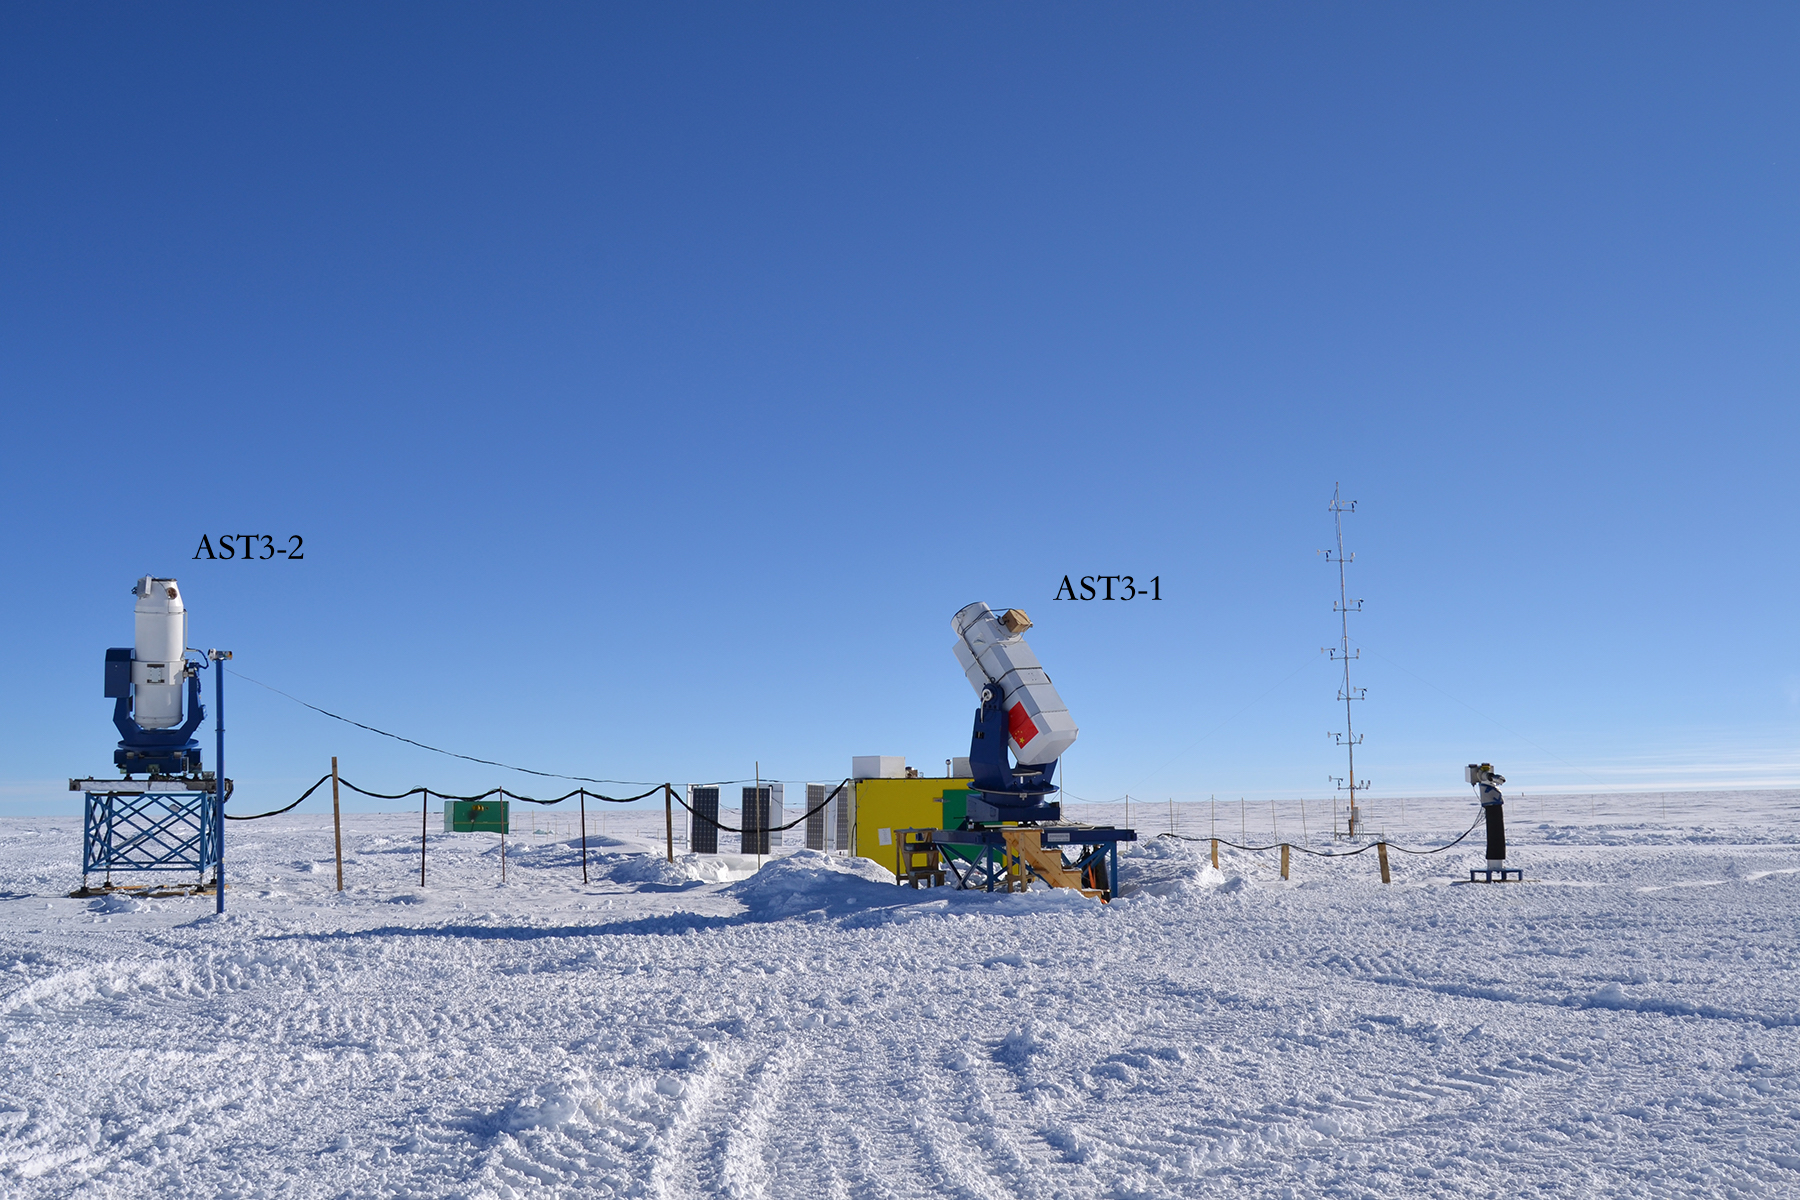
\includegraphics[width=1.0\textwidth]{figures/chapter2/f11_ast3.jpg}
\caption{AST3-2望远镜(左侧)就位于南极天穹 A 观测站。本图拍摄者为天文科考科考人员杜福嘉。}
\label{fig:ast3tele}
\end{figure}

\begin{enumerate}[leftmargin=1\parindent] 

\item[\tiny$\bullet$] \textbf{初始化输入} {} 整个观测自动化程序从这里开始。首先观测开始会生成当天的
日志记录。紧接着读取输入参数并检查文件系统是否正常。如果正常则读取我们的目标观测天区信息文
件,跳转到下一步自动观测流程。


\item[\tiny$\bullet$] \textbf{观测操作} {} 因为 AST3 有了一整套的望远镜跟踪系统,因而观测操作除了正
常的 CCD 曝光采集恒星图像文件以外,还额外需要控制望远镜的正常指向和信息反馈。特别是对与风雪
恶劣的天气,需要额外小心操作并及时采集错误。


\item[\tiny$\bullet$] \textbf{数据处理} {} 为了实时检测系统的工作状况,除了有一套实时摄像头对准 
AST3之外\footnote{远程实时检测网址\url{http://aag.bao.ac.cn/klaws/}。},我们还额外加入了远程定位
(astrometry)与测光(photometry)的模块。这部分环节和观测模块
各自独立运行,可返回非常实用的实时消光以及望远镜指向跟踪精度等信息。


\item[\tiny$\bullet$] \textbf{报错系统} {} 容错子系统是观测策略中必不可少的成分。以上描述的各个流程都会对错误守护进程实时反馈,一旦有错误报错系统会在当前操作结束后中断观测并向远程(如南京大学天文与空间科学学院远程观测实验室本地终端)传送错误信息。本地系统抓取到错误后也会立即通过邮件系统通知相关人员。

\end{enumerate}

\begin{figure}[t]
\centering
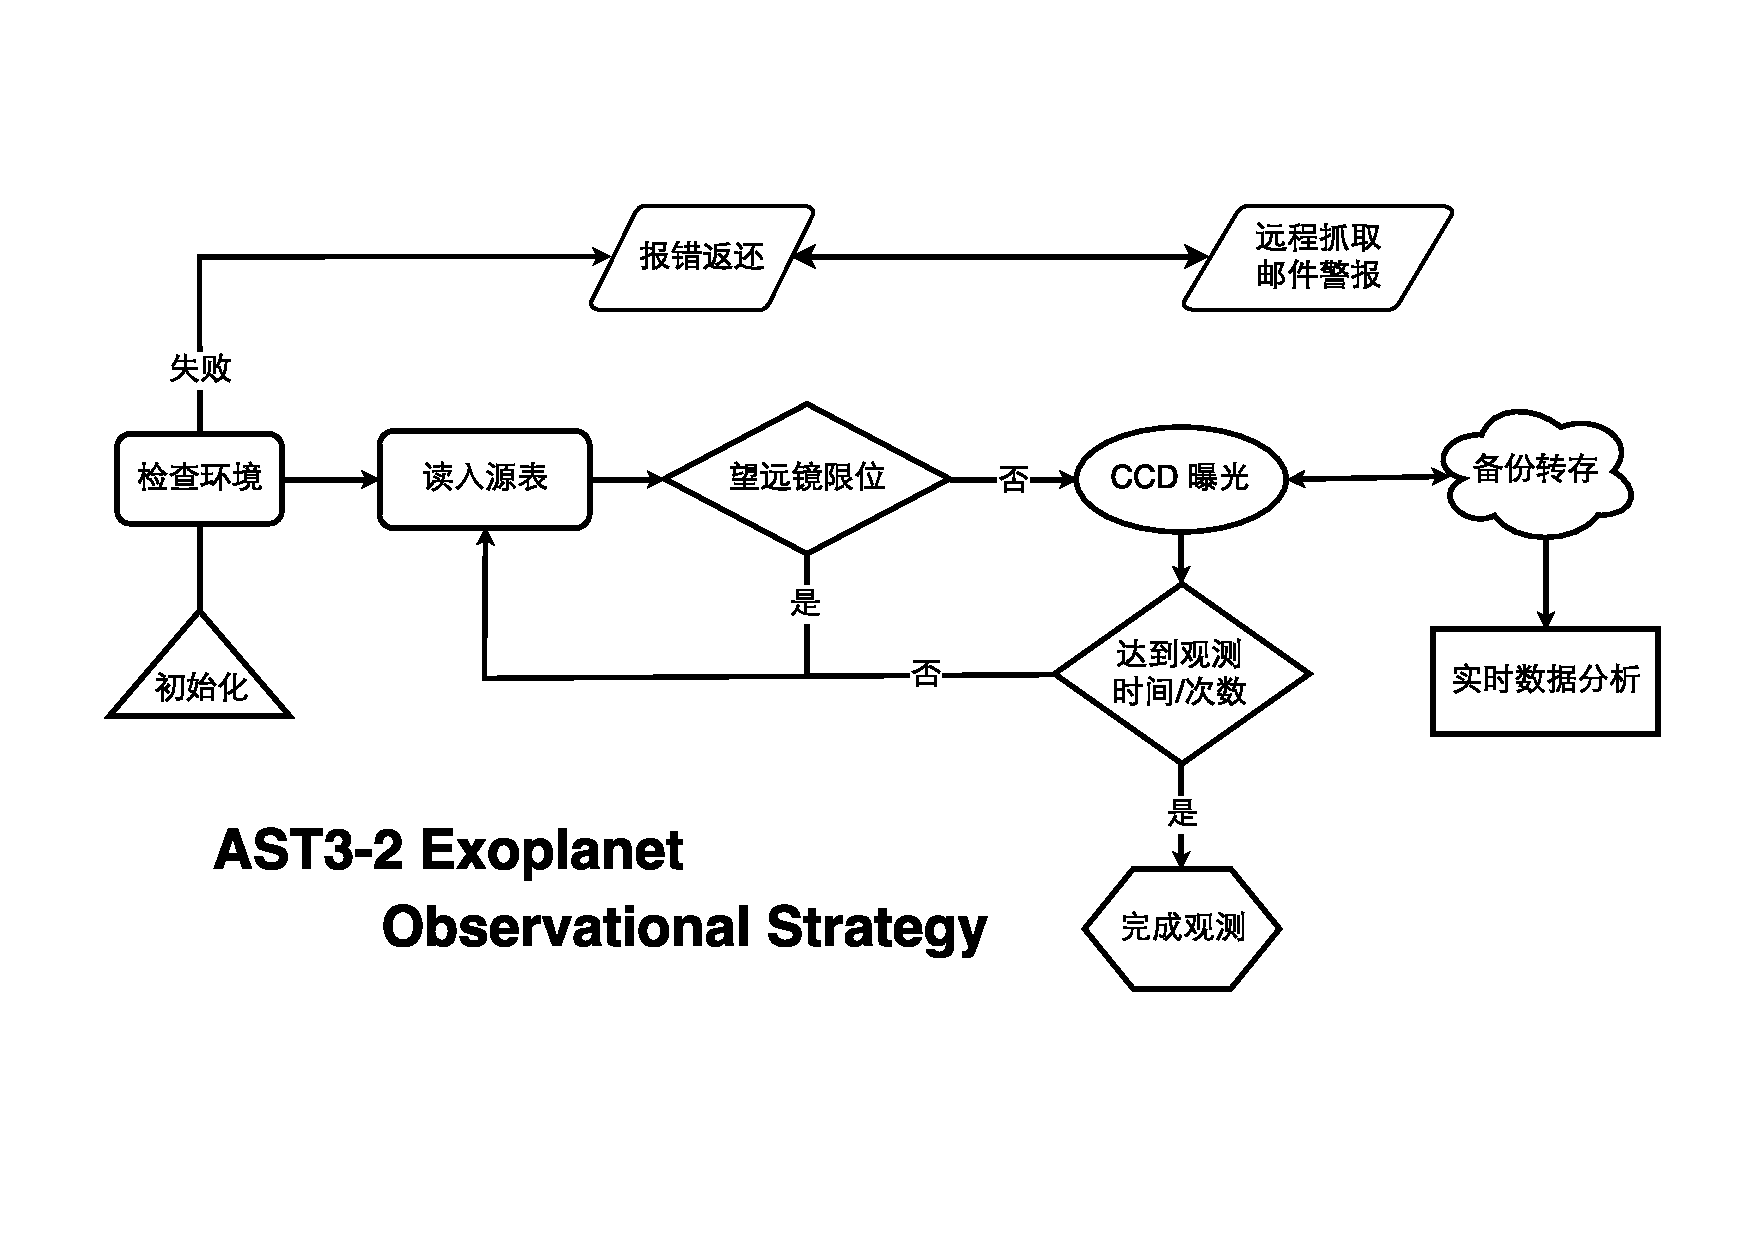
\includegraphics[width=1.0\textwidth]{figures/chapter2/f12_ast3pipeline.pdf}
\caption{AST3-2 观测策略。整体流程包括初始化输入,观测,容错以及数据处理共四个环节。}
\label{fig:ast3obs}
\end{figure}

充分完善以上流程\footnote{源代码链接 \url{https://github.com/meldonization/exoSurvey}。}对于保证观测(尤其是极地环境连续黑夜)非常重要,尤其是在 \S \ref{sec:pexample} 提到的极短周期行星探测以及性质刻画(Zhang et al. in prep.)。经过以上的充分实验,我们也完全有理由相信,随着今年科考人员采集数据归来,一批新的科学成果即将涌现。现有的包括 CSTAR 和 AST3 在天穹 A 台址的天文望远镜必定能助力今后即将诞生的昆仑暗宇宙巡天望远镜 KDUST,前人的观测以及数据处理也会一同作为试金石,铺助南极科学日益精进。



\chapter{利用掩食搜索双星中的星周盘} \label{chapter:form_evo}

\section{研究背景} \label{sec:diskbackground}

\subsection{星周盘简介} \label{sec:diskintro}

盘在天体物理中十分常见:从星系尺度的气体盘\cite{Binney1987,Gilmore1989}到致密星周围的吸积盘
\cite{Pringle1981},再小至行星形成的原行星盘(\S \ref{sec:pltfrmatntheory})以及形成卫星摇篮 --- 环
行星盘\cite{Smith1981,Latter2017,Mosqueira2003}。早在 17 世纪初盘,笛卡尔为了解释太阳系的行星
构型就引入了盘的概念,尽管那时候人类并未真正了解原恒星盘的模样\cite{Kawabe1993}。如今已迈入
中年的太阳系依然尚有黄道尘埃盘\cite{Dermott1994}、主小行星带以及库依柏带星子盘,这些也都是太
阳系纷乱的历史留下的残骸\cite{Dohnanyi1969}。


\begin{figure}[b]
\centering
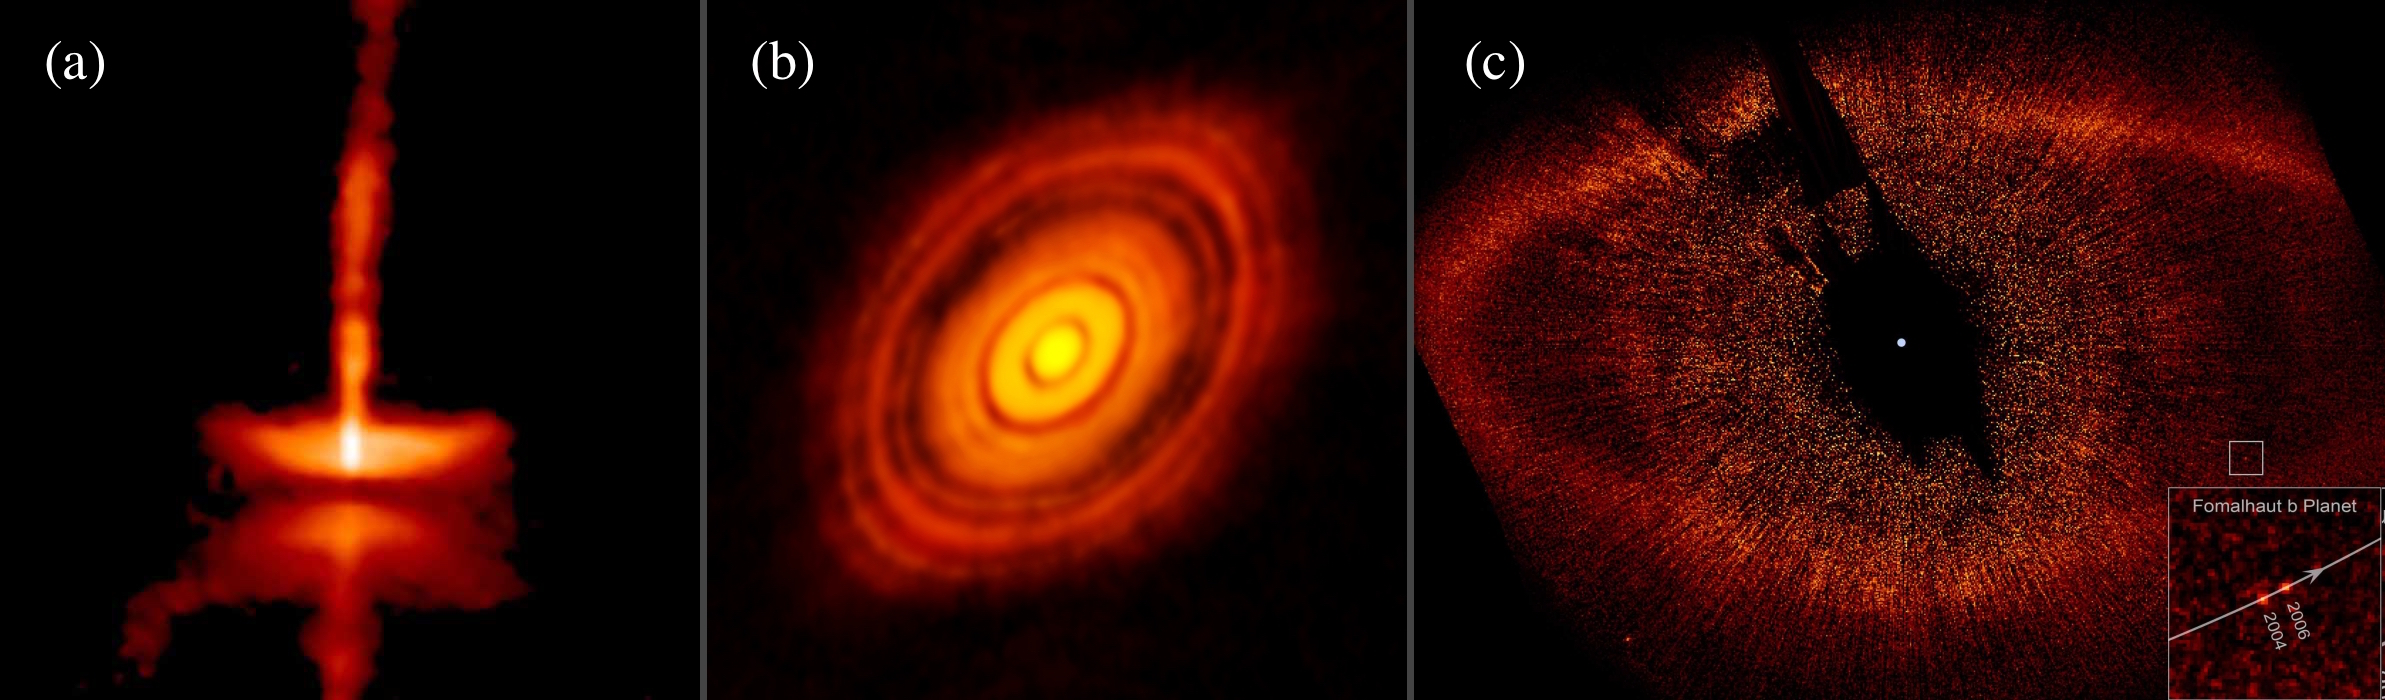
\includegraphics[width=1.0\textwidth]{figures/chapter3/f2_obsdisc.jpg}
\caption{原行星盘从早期、过渡到晚期三个不同的形态,其中 \textbf{(a)} HH 30 侧向视角的临变增厚盘,双极喷流清晰可见(版权:NASA, Alan Watson) \textbf{(b)} HL Tau (版权:ALMA - ESO/NAOJ/NRAO) \textbf{(c)} Formalhaut 残骸盘(版权:NASA,ESA 和 P. Kalas 等)。}
\label{fig:obsdisc}
\end{figure}

\begin{figure}[ht!]
\centering
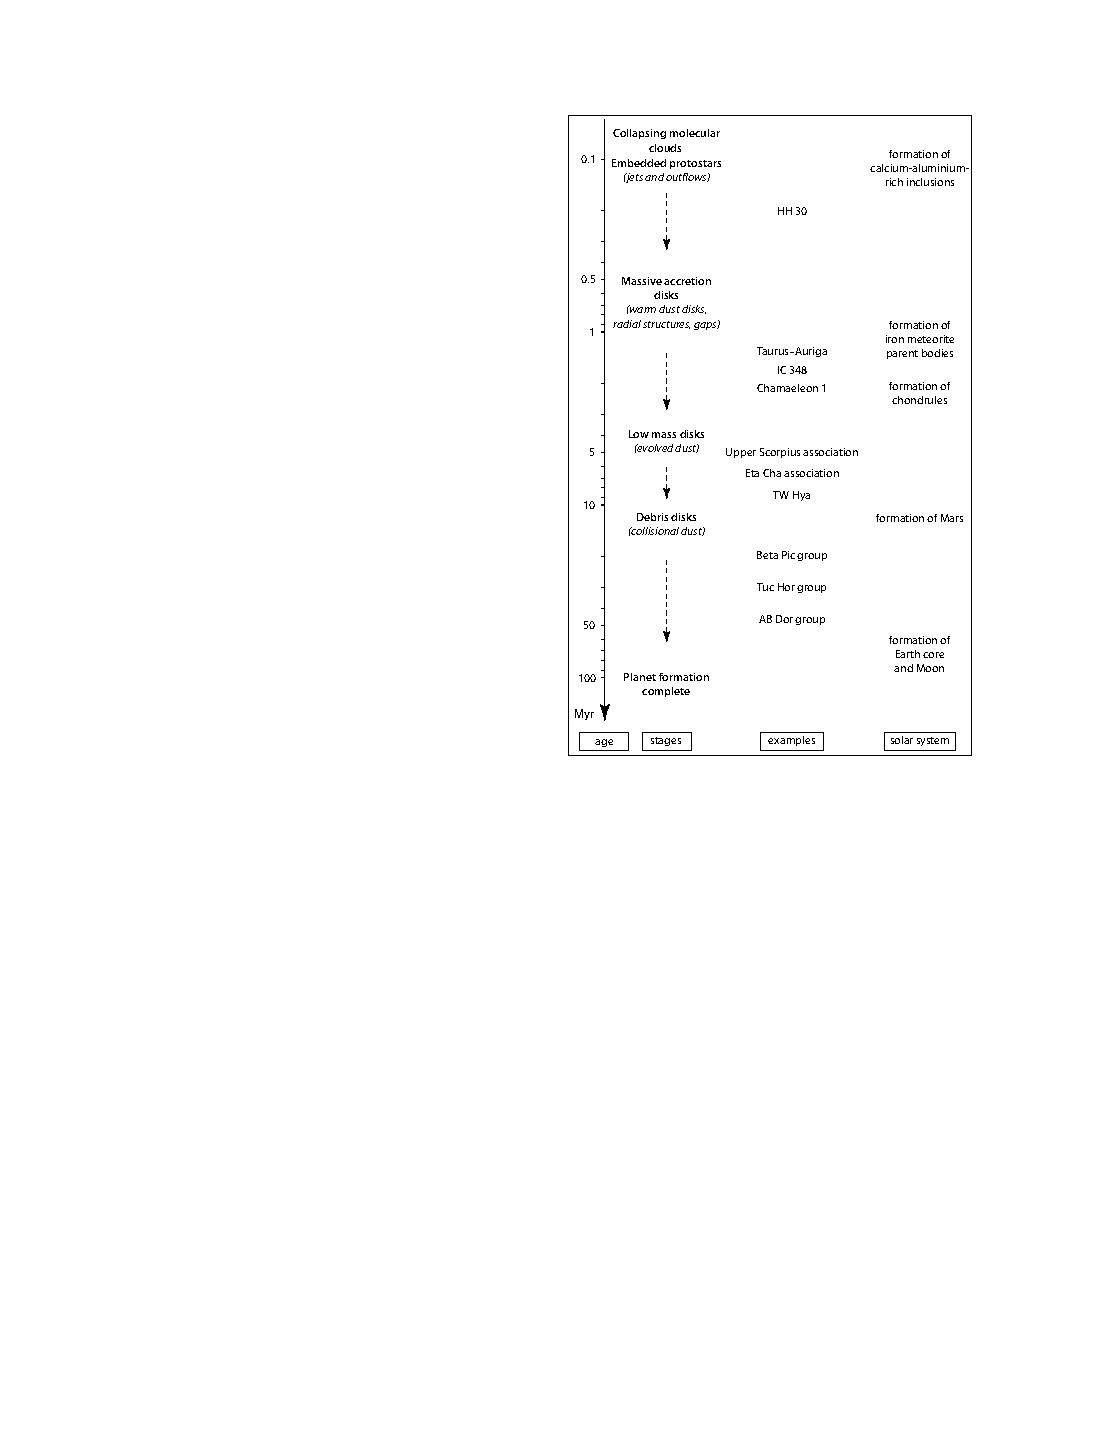
\includegraphics[scale=1.8]{figures/chapter3/f1_pfdisc.pdf}
\caption[行星形成的不同时期快照,从左至右分别为物理时间、形成阶段、系外行星系统实例与太阳系历史,版权所有人 Perryman。]{行星形成的不同时期快照,从左至右分别为时间、形成阶段、系外行星系统实例与太阳系历史。图片采取自书籍\citen{Perryman2014exohb},更详细的图请查看书籍\citen{ApaiLauretta2010}。}
\label{fig:pfdics}
\end{figure}


正如前文(参考\S \ref{sec:pltfrmatntheory})提到,行星孕育在星周盘内。此过程(如图 \ref{fig:obsdisc} 
与 \ref{fig:pfdics} 所示)包括早期分子云坍缩、恒星吸积盘内固体沉降、气体消散行星形成和最终演化为
残骸盘(Debris disk,又称碎屑盘)几个阶段。一般而言,描述气体的过程为内盘区域等离子磁层作用与
外层气体辐射转移两个过程\cite{Dullemond2010},而脱离气体耦合作用后的固体盘
一般则为 N 体引力作用(\S \ref{sec:clspftheory})。

星周盘(Circumstellar disk)观测到的辐射在理论上一般会用多黑体辐射谱来拟合。普朗克黑体谱
(Black body)有如下形式:

\begin{equation} \label{eq:blackbody}
\tif{B}_\nu (\tif{T}) = \frac{2h\nu^3}{c^2} \, \frac{1}{e^{h\nu / k\tif{T}}-1}
\end{equation} %myequation{黑体辐射}

\begin{figure}[t!]
\centering
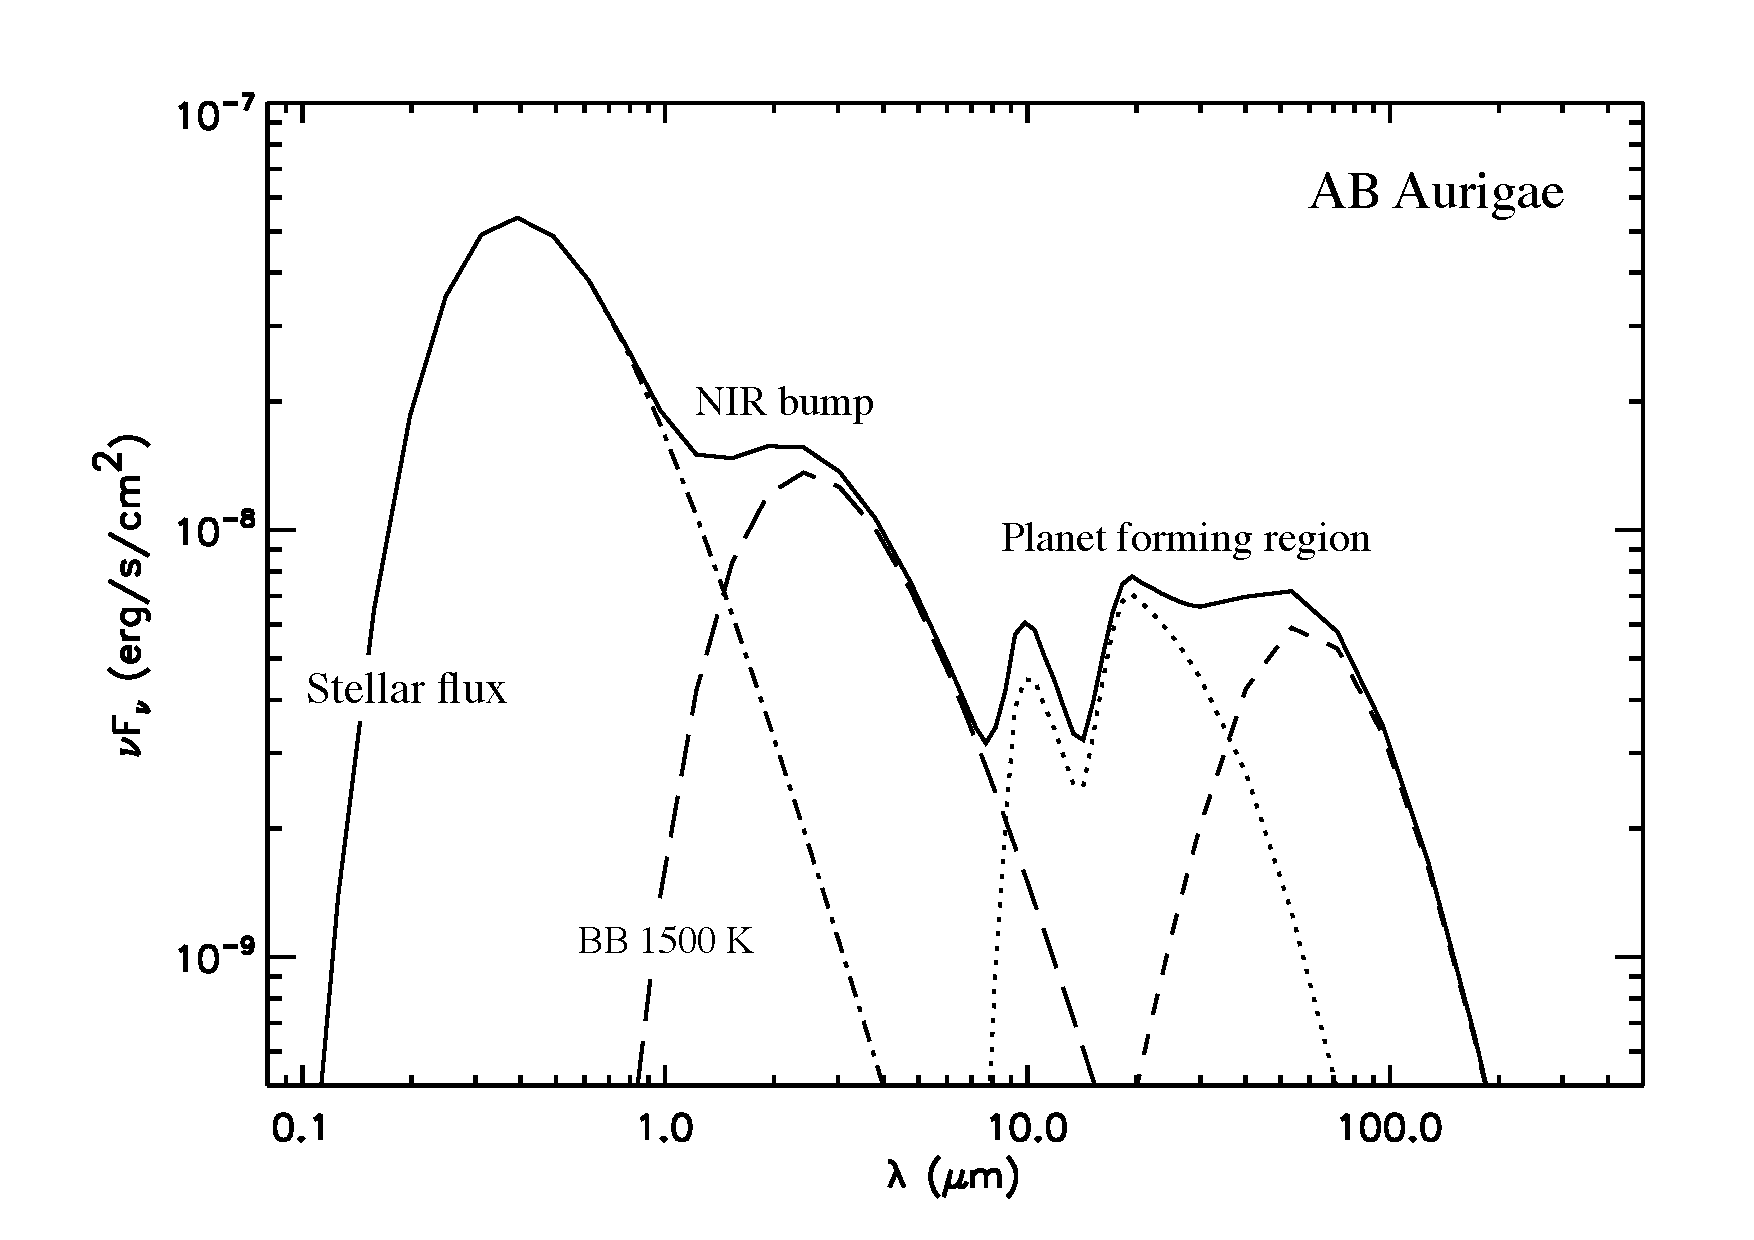
\includegraphics[width=1.0\textwidth]{figures/chapter3/f3_youngdisc.pdf}
\caption[AB Aurigae 系统理论谱能量分布图。从左至右分别表示恒星、有效温度为 1500 K 的星周内侧盘与外侧行星形成区域的黑体辐射组分。该图利用 Dullemond 开发的 CGPlus 程序制作。]{AB Aurigae 系统理论谱能量分布图。从左至右分别表示恒星、有效温度为 1500 K 的星周内侧盘与外侧行星形成区域的黑体辐射组分。此图利用 Dullemond 开发的 CGPlus 程序\footnotemark[1]制作。}
\label{fig:transdiscsed}
\end{figure}
\footnotetext{链接 \url{http://www.mpia.de/homes/dullemon/radtrans/fitcgplus/}。}

同样,径向对称且几何薄的星周盘总辐射可看作每个环状细盘黑体辐射的积分叠加,形式如下:

\begin{equation} \label{eq:diskrad}
\tif{F}_\nu = \frac{\cos \theta}{\tif{D}^2} \, \int \tif{B}_\nu (\tif{T}_\tif{d}) \, ( 1-e^{-\tau} ) \, 2\pi r \tif{d} r \ ,  
\end{equation} %myequation{盘总辐射量}
其中 $\theta$ 为观测者的视角,D 为观测者和源之间的距离。光深 $\tau$ 与盘内尘埃的不透明度
(Opacity)以及盘的面密度分布有关,因而上述公式所描述的星周盘谱能量分布(SED)函数是高度简并的函数。

%\begin{figure}[t]
%\centering
%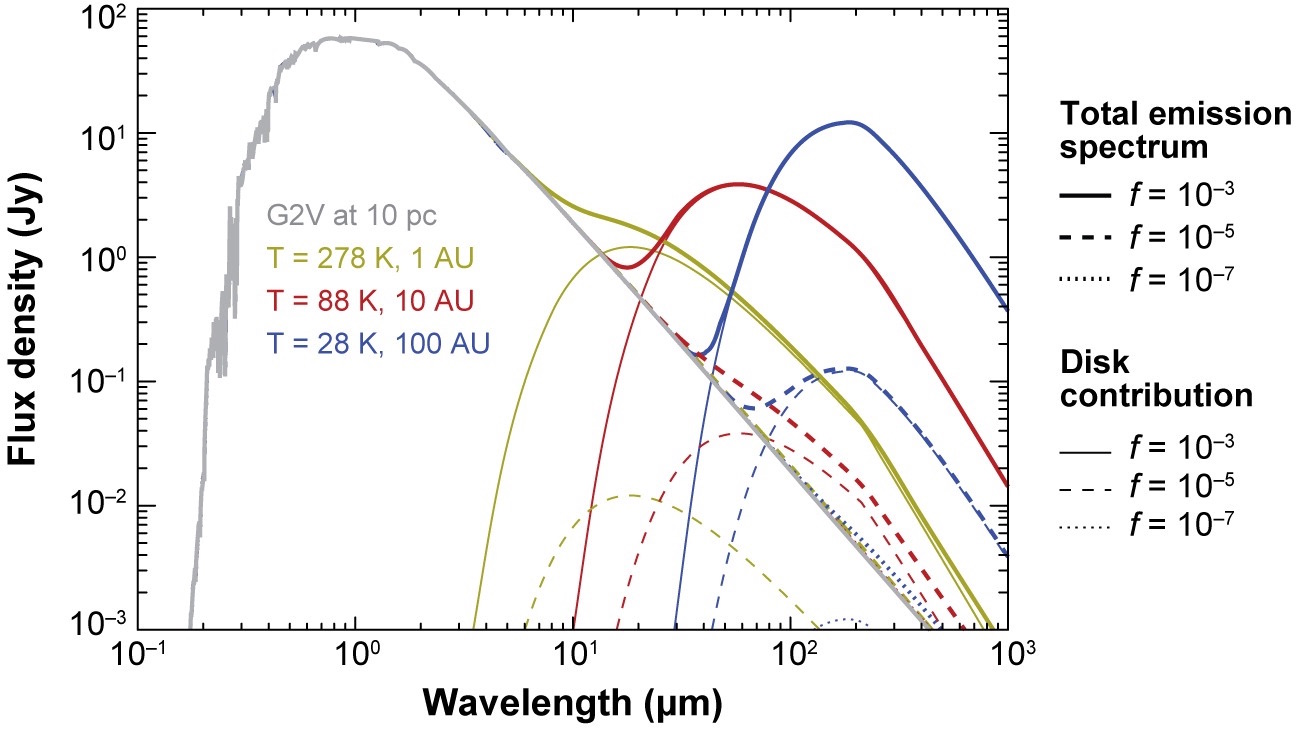
\includegraphics[width=1.0\textwidth]{figures/chapter3/f4_debrisdisc.jpg}
%\caption[类太阳(G2V)恒星于 10 pc 以外的理论辐射谱能量函数,长波范围的鼓包为星周残骸盘的黑体辐射。图片版权归 Wyatt 所有。]{类太阳(G2V)恒星于 10 pc 以外的理论辐射谱能量函数,长波范围的鼓包为星周残骸盘的黑体辐射。图片取自文献\citen{Wyatt2008}。}
%\label{fig:debrisdiscsed}
%\end{figure}


图 \ref{fig:transdiscsed} 为我们展示的为一个典型的原初恒星盘(Primordial disk)的能谱分布。此时从
内至外(波长由短至长),该 SED 主要包括四种成分:主星(9000 K)的黑体辐射,星周盘内侧区域
有效温度约 1500 K 的黑体辐射(近红外突起),行星形成区域(约从 1 AU 至 10 AU的尘埃连续谱)以
及最外侧亚毫米波段的盘最外侧。盘的演化是一个自内向外的消散过程,在观测中随着星周盘从原初恒
星盘演化至内侧区域最先被清空从而成为过渡盘(耗散相对快速,可被 ALMA 连续谱或成像观测
\cite{WilliamsCieza2011}),再最终演化成残骸盘(可被 HST 观测\cite{Wyatt2008})。需要说明的是,
由于星周盘的尘埃辐射主要集中在红外或更长的波段,所以观测中一般也将上述流量描述为红外光度比
例 $\tif{L}_\tif{IR}/\tif{L}_\tif{s}$。


\subsection{双星中星周盘研究背景} \label{sec:diskintro}

双星和多星系统在银河系中非常普遍,巡天显示类太阳恒星的成双概率大致为 45\%,并且其中约有 
10\% 为三星或更多星系统(文献 \citen{Duquennoy1991})。在双星系统形成早期,某一颗恒星可能会
拥有星周盘\cite{Bate1995},当观测者从远处观测时,会有一定的概率看到星周盘遮挡住此系统另外一
颗恒星。由于盘的尺度相比于恒星的尺度高出许多量级,因而一个随机取向的含盘系统可能会有非常高
的几何掩食概率\cite{Mamajek2012}。这样的掩食盘可以存在于行星形成中的双星系统(文献 
\citen{Galan2012})或卫星形成中的行星系统(文献 \citen{Mamajek2012})。掩食盘可以为我们提供非
常丰富的独到信息,如盘的不透明度以及三维立体结构(如土星环掩食,文献 \citen{Hedman2007})。

在观测上,$\epsilon$ Aurigae\cite{Guinan2002,Kloppenborg2010,Chadima2011} 与 EE Cephei 
\cite{Mikolajewski1999,Graczyk2003,Mikolajewski2005,Galan2012} 是两个相对熟知的盘状掩食双星系
统。最近 Mamajek 探测到太阳质量主序前恒星周围长时间、大深度的复杂盘掩食事件
\cite{Mamajek2012}。

在大麦云(Large Magellanic Cloud,下文简称 LMC)的掩食双星(EBs)中,Udalski 等人
\cite{Udalski2008,Graczyk2011}利用 OGLE-III 巡天发现了周期为 13.3 天的光变曲线中存在疑似盘结构
的系统 OGLE-LMC-ECL-17782,文献 \citen{Derekas2007} 曾认为此系统是不接食双星(Eclipsing 
Detached Binary,简称 ED)。在同一巡天计划样本中,拥有 468 天周期的系统 OGLE-LMC- 
ECL-11893 也被怀疑为掩食盘\cite{Dong2014}。下文,我们将利用 OGLE-III 巡天数据中 LMC 与 小麦
云(Small Magellanic Cloud,或简称 SMC)以及银盘(Galactic Disc,下文统称 GD)观测到的 EB 样
本\cite{Graczyk2011,Pawlak2013,Pietrukowicz2013} 光变曲线中分析额外可能的掩食盘事件。

近年来,对太阳附近恒星以及恒星形成区的红外以及毫米波段巡天显示恒星的年龄、质量以及伴星的存
在会影响恒星周围是否存在可探测的盘状结构
\cite{Haisch2001,Bouwman2006,Hernandez2007,Harris2012,DeRosa2013}。在对 OGLE-III EB 的研究
显示 EB 系统在大型巡天中是一个近乎确定、完备的样本
\cite{Graczyk2011,Pawlak2013,Pietrukowicz2013}。另外,我们还将本文 LMC  EB 掩食盘的搜寻概率与
近年已有的银河系红外(毫米波)的盘探测率做了对比。这种另辟蹊径的做法也可能为今后搜寻活动提
供新的导向。

\section{利用双星掩食光变曲线搜索星周盘} \label{sec:discsineb}

文献 \citen{Graczyk2010} 提到利用光变曲线中星等分布(或者统计矩阵)可以区分不同的变星以
及 EBs。根据他们的方案,我们在 EBs 的光变曲线的在食区间使用同样的方法,目标是将以往 EB 系统
中可能的掩食盘结构区分并探测出。在 EBs 中,其中一颗掩食另外一颗星通常会造成一个三角、方形或
者高斯轮廓的掩食光变曲线。在本文,我们则利用光变曲线中和这些普通情况不同的掩食形状来区分可
能的掩食盘系统。这些结构包括不对称型(EE Cep 或 J1407,文献 
\citen{Galan2012,Mamajek2012}),W-型掩食形状($\epsilon$ Aurigae,文献 \citen{Guinan2002} )
或者宽平台型(如 OGLE-LMC- ECL-17782,文献 \citen{Graczyk2011})。如果我们探测到此类特殊结
构,我们则会将该系统标注为掩食盘候选体,尽管我们并未真正看到盘本身的旋转结构。


\subsection{搜索掩食盘的方法} \label{sec:discebmeth}

下面我们将简要介绍搜索掩食盘的过程,该过程不仅可以利用于 OGLE-III LMC,SMC 和 GD 的 EB 样
本,也可以推广至任何其他的巡天中。

\begin{enumerate}
\item 提取 OGLE-III 巡天中被识别成 ED 系统的相位叠加光变曲线,并计算该曲线的平均星等值与掩食
外光变曲线平台的弥散值;
\item 抛弃信噪比太低、观测点数太少或光变曲线平台部分弥散值太大(暗示此源可能为变星)的系统;
\item 利用程序自动识别主掩食和次掩食以及它们彼此互掩开始(初亏)和结束(复圆)的位置,这样便
可确定光变曲线掩食内的窗口;
\item 计算掩食内光变曲线的斜度(Skewness)与峰度(Kurtosis)以及星等的分布统计值。
\end{enumerate}

我们并没有考虑低信噪比、观测点太少的光变曲线,因为此类系统的在食部分并不能被有效地识别出。
这部分系统的斜度和峰度参数不能被很好的反演,从而造成成倍的额外掩食盘「假阳性」候选体。而如
何计算这些 EBs 系统掩食外的星等标准差以及识别进食(ingress)和出食(egress)粗略介绍如下:


\begin{enumerate}
\item 首先,我们将 OGLE-III 巡天计划中的 LMC,SMC 和 GD 得到的 EDs 光变曲线在它们各自的轨
道周期\cite{Graczyk2011,Pawlak2013,Pietrukowicz2013}上做折叠;

\item 接下来计算整条光变曲线(掩食内以及掩食外)的中值(median value),并记作 $\mu_\tif{L}$。
因为这边取的是中值,从而此值应大约为 EB 光变曲线掩食外的平均星等;

\item 然后对整条光变曲线做宽度为五个点的点滑动平均(box smoothing),将最暗(星等值最大)的
点标记为主掩食甚(伴星遮挡主星面积最大的时刻),用 $\theta_\tif{p}$ 表示。而次掩食甚时刻 $
\theta_\tif{s}$ 则定义为在 $\theta_i$ 处,$|m(\theta_i) - m(\theta_\tif{m})|$ 达到最大值,其中 $
\theta_\tif{m}$ 等于 $(\theta_i+ \theta_\tif{p})/2$,而 $m(\theta)$ 为相位 $\theta$ 处的星等值;

\item 选取在 $[\theta_\tif{m} - 0.05, \, \theta_\tif{m} + 0.05]$ (也即绝对相位宽度为 0.1)区间内计算这
段光变曲线的标准差:$\sigma_\tif{L}$,也即掩食外光变曲线的弥散度;

\item 而光变曲线的主掩部分则定义为星等值比平均值低 $1\sigma$,即 $m > \mu_\tif{L} + \sigma_\tif{L}
$ 并且区间内包含 $\theta_\tif{p}$. 同样的方法也可以定义包含 $\theta_\tif{s}$ 的次掩食部分。

\item 最后将上步得到的两段主次掩食内的光变曲线从整条光变曲线中扣除,并重新计算第 2 步中的中值
以及弥散。这样做可以得到更加真实的光变曲线掩食外部分。利用新得到的 $\mu_\tif{L}$ 和 $\sigma_
\tif{L}$,我们可以在再次回到上一步划分主次掩内的光变曲线。值得注意的是这里得到的 $\mu_\tif{L}$ 
和 $\sigma_\tif{L}$ 两者之值将被用来计算掩食内光变曲线的斜度和峰度。
\end{enumerate}

\begin{figure}[ht!]
\centering
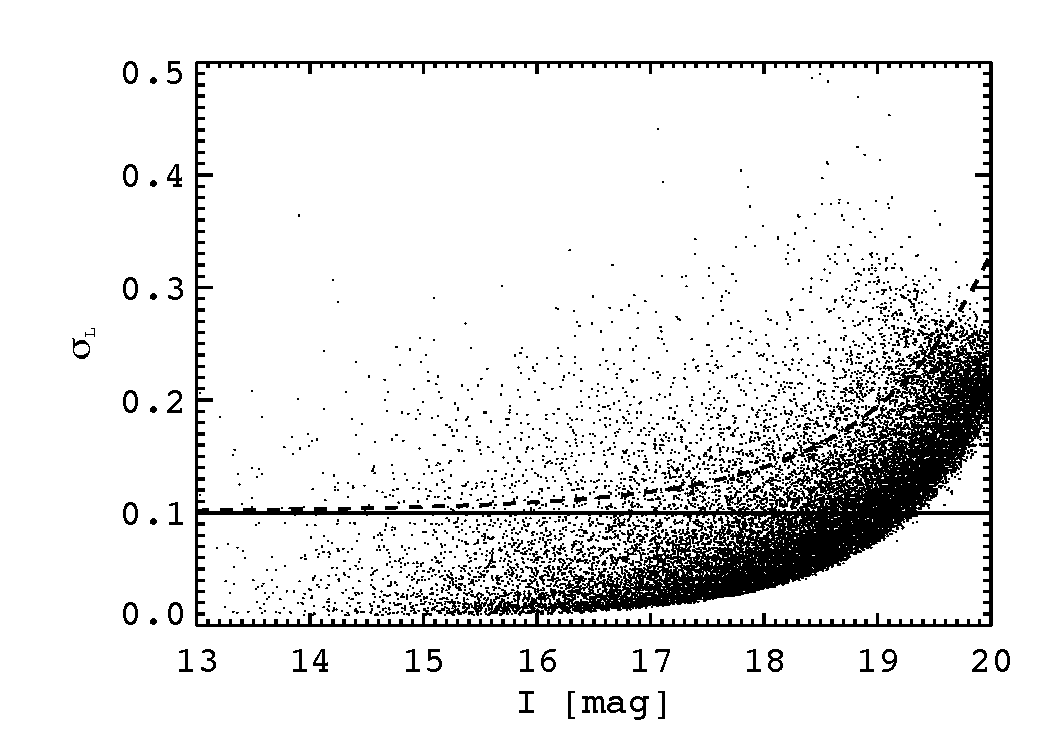
\includegraphics[width=1.0\textwidth,trim={0.4in 0.2in 0 0}]{figures/chapter3/f4_magerr.pdf}
\caption{OGLE-III LMC EBs 样本 $i$ 波段星等与该波段掩食外的星等标准偏差散点图。为了着重显示高信噪比的系统,我们人为去除了 $i$ 波段星等大于 19.3 的 EBs。另外实线上侧的掩食外星等弥散度 $\sigma_\tif{L} > 0.1$ 也被舍去。另外,虚线表示 $\sigma_\tif{L} > \sigma_\tif{c} + 0.1 $,其中 $\sigma_\tif{c}$ 为极限星等误差。我们也尝试过该选择判据,结果显示两种方法并不能影响图 \ref{fig:lmcks} 中的实线方框内的点。}
\label{fig:magerr}
\end{figure}

下面我们将以 OGLE-III LMC 内共 26,121 个 EB 样本\cite{Graczyk2011}为例,介绍如何得到可靠的斜度
和峰度。图 \ref{fig:magerr} 为对该样本计算得到的 $\sigma_\tif{L}$ 与 $i$ 波段星等的分布函数图。从图
中可以明显看到信噪比较差的系统总是暗源,这也很自然,因为测光误差总是依赖于星等。为了避免用来
搜寻掩食盘的样本性噪比太低,我们将 $i$ 波段测光星等大于 19.3 以及弥散大于 0.1 的系统从样本中剔
除。

另外,如果掩食窗口内的观测点数太少,我们也同样不能精确的计算星等分布的多极矩。如果在掩食窗口
内光变曲线的点数为 $N_\tif{ecl}$,那么 $N_\tif{ecl}/N \le 0.25$ 的系统也会被排除在外,其中 $N$ 为整
个光变曲线的观测点数。此选择条件还可以将我们的样本限制为 EDs。而且为了保证斜度和峰度计算值
的可靠度,只有 $N_\tif{ecl} > 20$ 的系统才会被留下来用作下一步的计算。最后,我们还将分析的系统
限制在较深的掩食中。为了寻找主掩食盘(即伴星的星周盘),我们的分析中只留下光变曲线主掩深度 $|
m(\theta_\tif{p}) - \mu_\tif{L}| > 4 \sigma_\tif{L}$ 的系统,其中 $|m(\theta_\tif{p})  - \mu_\tif{L}|$ 用来衡量
主掩食深度。同样次掩食盘(主星的星周盘)判据则定为 $|m(\theta_\tif{s}) - \mu_\tif{L}| > 3 \sigma_
\tif{L}$。之所以这样选取是因为当以上两个判据变得不那么严格时,最后的结果中会包含相当多的污染源
以至于掩食盘候选体被淹没在其他系统中,这些系统并没有掩食盘而只是星等分布接近掩食盘系统。

在主掩和次掩食内,星等分布的斜度 S 以及峰度 K 的计算公式如下:

\begin{equation} \label{eq:skew}
S =  \frac{1}{N} \sum_{i=0}^{N-1} \left(\frac{m_i - \mu}{\sigma_\tif{L}}\right)^3 
\end{equation} %myequation{样本高阶矩 --- 斜度的计算公式}
\begin{equation} \label{eq:kur}
K =  \frac{1}{N} \sum_{i=0}^{N-1} \left(\frac{m_i - \mu}{\sigma_\tif{L}}\right)^4 - 3 \, \ , 
\end{equation} %myequation{样本高阶矩 --- 峰度的计算公式}
其中掩食窗口内的星等平均值 $\mu = \frac{1}{N} \sum_{i=0}^{N-1} m_i$。需要留意的是这边的平均星等 
$\mu$ 和前一小节的中值 $\mu_\tif{L}$ 不能混为一谈。$N$ 为掩食窗口内折叠后光变曲线的观测点数
目,而 $m_i$ 则是它们中每一个观测点的星等值。


\begin{figure}[t]
\centering
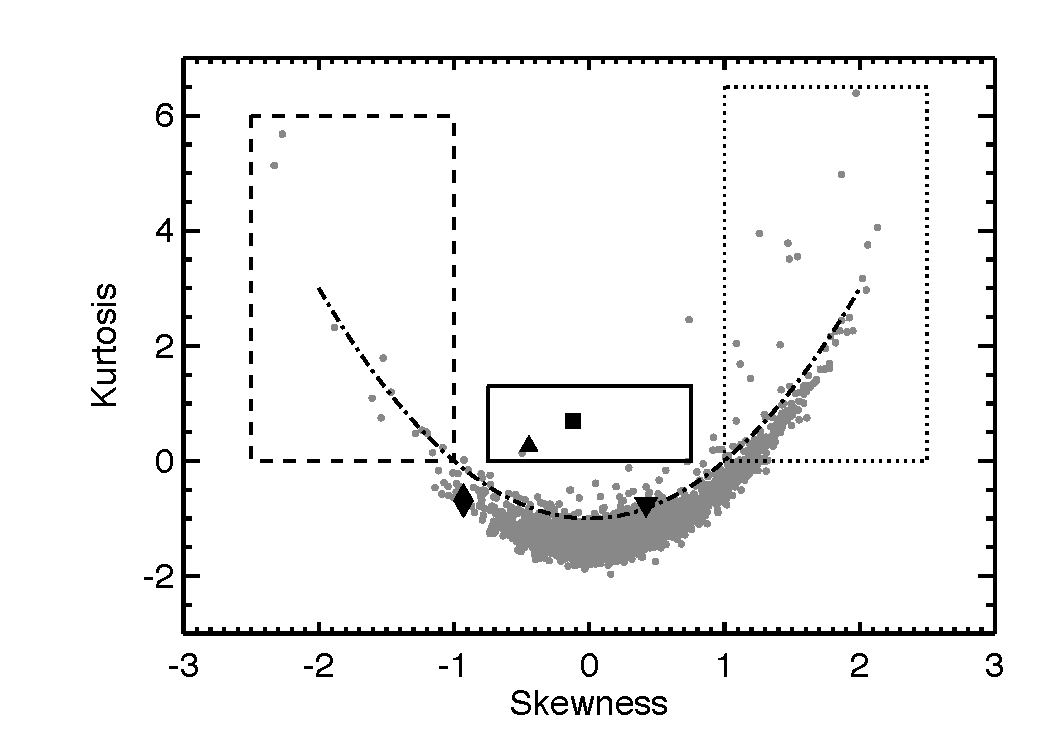
\includegraphics[width=1.0\textwidth,trim={0.4in 0.2in 0 0}]{figures/chapter3/f5_lmcks.pdf}
\caption{由 LMC 中 2823 个低噪声 EBs 样本计算得到的主掩食内斜度和峰度分布图。OGLE-LMC-ECL-17782 和 OGLE-LMC-ECL-11893 分别用实心方块与三角形标注。为了区分不同性质的系统,我们将该图划分为四个不同的区域:虚线、实线、点线以及点虚线,它们分别代表着拥有不同掩食内光变曲线形状的 EBs --- 实线区域内为掩食盘的候选体,而点虚线(近似 $K=S^2-1$ 抛物线)则为星等分布的整体形状。EE Cep 和 $\epsilon$ Aur 也分别用倒三角与菱形标注,可以看到斜度峰度方法并不能很好的区分 EE Cep 和 $\epsilon$ Aur 和其他 EBs。}
\label{fig:lmcks}
\end{figure}


\subsection{掩食窗口内星等分布} \label{sec:discebresult}

我们首先尝试将上述方法运用到 OGLE-III 巡天中 LMC EBs 的样本\cite{Graczyk2011}。OGLE-III 巡天在
凝视 LMC 的视场大约有 40 平方度的大小,视场内也探测到近 320 万个源\cite{Ulaczyk2012}。其中 
26,121 个源被证认为 EBs\cite{Graczyk2011}。为了从大量数据中搜索这些双星,Graczyk 和 Eyer 将 $i$ 
波段的星等限制在 20 以内,至少拥有 120 个测光点,并且周期限定在 $1.0015 < P< 475$ 天
\cite{Graczyk2010},他们搜索这些双星的周期运用了 Stellingwerf 提出的 phase dispersion minimization 
方法\cite{Stellingwerf1978}。

上一小节提到选取限定条件,于是我们从 LMC 26,121 个系统中挑选出了 2823 个高测光连续度且测光精
度较好的 EB 系统,这些系统被成为高信噪比 LMC EBs。计算出这些高信噪比 LMC EBs 的斜度以及峰
度后(图 \ref{fig:lmcks} 中),之前两个已发现的掩食盘系统 OGLE-LMC-ECL-17782 和 OGLE-LMC-
ECL-11893 落在了实线方框区域($|S| < 1.0$,$K > 0$)。同样,我们定了双曲线 $K = S^2 - 1$(以指
代普通 EBs)来区分主掩和次掩食内是否明显有平台期。这里明显的判断标准则落在了 $S = 0$ 和 $K = 
0$ 附近。类似的对于系统 EE Cep 与  $\epsilon$ Aur,我们采用了 Galan 等人\cite{Galan2012}观测到的 
V 波段掩食数据\footnote{\url{http://vizier.cfa.harvard.edu/viz-bin/VizieR?-source=J/A+A/544/A53}}和 
Parthasarathy 于 1982 至 1988 年之间\cite{Parthasarathy1986}观测的 V 波段数据\footnote{\url{http://
www.hposoft.com/campaign09.html}} 来计算斜度和峰度,然而他们并没有很好的和其他系统分离开。

那么究竟什么原因导致上述 OGLE-LMC-ECL-17782 和 OGLE-LMC-ECL-11893 两个系统在斜度 --- 峰度
分布图中明显突出呢?从方程 \ref{eq:skew} 和 \ref{eq:kur} 出发,在统计中峰度可以用来指示星等分布的
集中度,而斜度则用可类比为星等分布的不对称度(即星等峰值在其平均值的明或暗两端)。正是如此,
我们才将图 \ref{fig:lmcks} 划分成四个区域:实线、点线、虚线和其余区域。点线区域内 EBs 掩食内星等
的分布集中在进出掩食附近,因此拥有正斜度(例如系统 OGLE-LMC-ECL-02192,参考图 
\ref{fig:lmc02192})。而虚线方框内 EBs 则因拥有方形平台底部贯穿最大掩食(食甚)而正好拥有相符号
反的斜度(例如系统 OGLE-LMC-ECL-12966,参考图 \ref{fig:lmc12966})。

\begin{figure}[t]
\centering
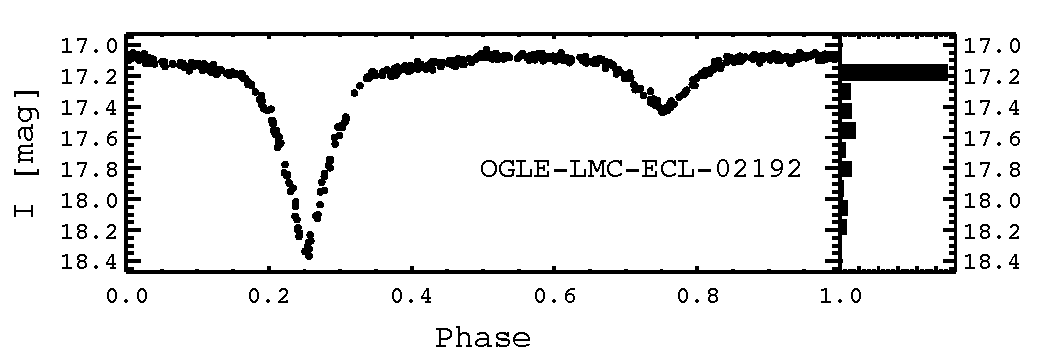
\includegraphics[width=0.98\textwidth,trim={0.0in 0.2in 0 0}]{figures/chapter3/f6_lmc02192.pdf}
\caption{OGLE-LMC-ECL-02192 的周期($P = 1.59\, \tif{d}$)叠加光变曲线(左侧),该系统属于 ED,并且其中一颗恒星的洛希瓣被充满。右栏为掩食内星等分布柱状图,入食与出食相位分别为 0.1 和 0.5。该系统入出掩食较缓慢,星等分布拥有明亮尾巴,因而拥有正斜度($S=1.94$,$K=4.98$),在图 \ref{fig:lmcks} 中处于点线方框内。}
\label{fig:lmc02192}
\end{figure}

如果系统中拥有可能的掩食盘候选体,那么光变曲线中掩食内的星等统计分布则与上述两种情况完全不
同。通常而言这样的系统会在光变曲线侧翼中(掩食半遮掩状态)包含平台状的结构。这也并不难理解,
因为盘的几何尺度往往比恒星尺度大,在伴星掩食主星之前,伴星周围的盘会先开始掩食。如果盘的结构
不复杂(多环、倾斜或单边状),那么在恒星掩食开始前会有一段盘掩食的平坦光变区间,这也正是系统 
OGLE-LMC-ECL-11893(图 \ref{fig:lmc11893})和 OGLE-LMC-ECL-17782(图 \ref{fig:lmc11782})与
图 \ref{fig:lmcks} 中其他 EBs 的不同之处。

\begin{figure}[t]
\centering
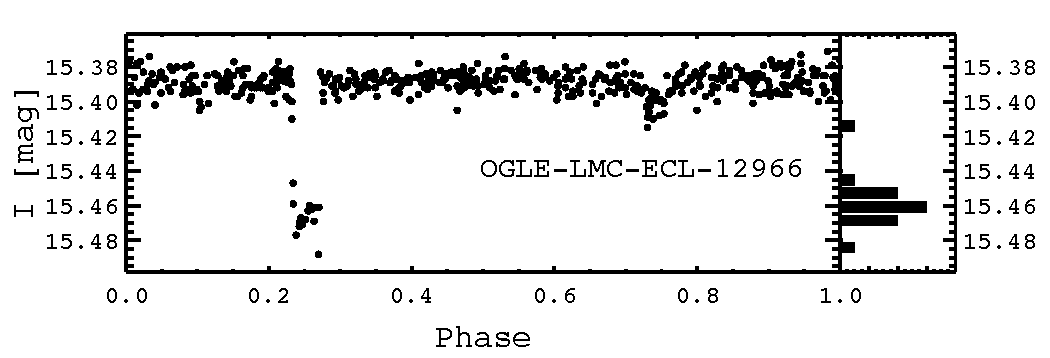
\includegraphics[width=0.98\textwidth,trim={0.0in 0.2in 0 0}]{figures/chapter3/f7_lmc12966.pdf}
\caption{与图 \ref{fig:lmc02192} 相同,但为系统 OGLE-LMC-ECL-12966($P = 239.6\, \tif{d}$)。该系统同样为 ED,但不同的是由于掩食内光变曲线呈方波形状,从而右侧星等分布集中在暗端,斜度也因此为负值($S=-1.35$,$K=1.21$)。在图 \ref{fig:lmcks} 中位于虚线框内。}
\label{fig:lmc12966}
\end{figure}


\begin{figure}[ht!]
\centering
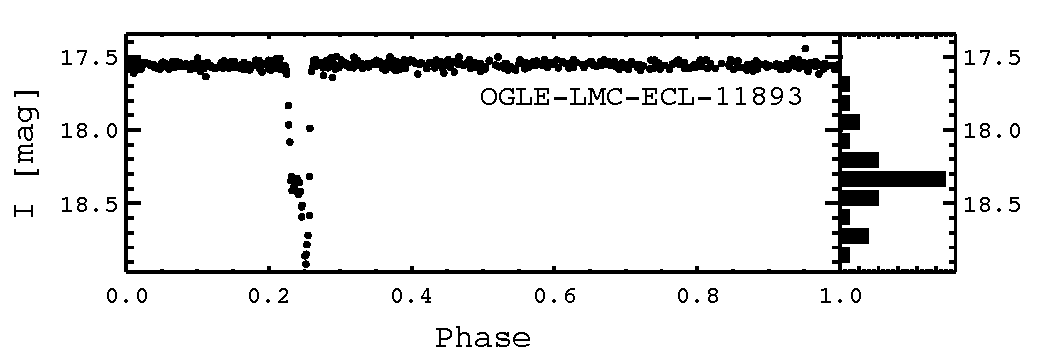
\includegraphics[width=0.98\textwidth,trim={0.0in 0.2in 0 0}]{figures/chapter3/f8_lmc11893.pdf}
\caption{与图 \ref{fig:lmc02192} 相同,但为系统 OGLE-LMC-ECL-11893($P = 468.045\, \tif{d}$)。该系的星等分布拥有斜度接近于零和正峰度($S=-0.45$,$K=0.25$),这是因为掩食内中央区域有一段平台期,在图 \ref{fig:lmcks} 中位于实线框内。}
\label{fig:lmc11893}
\end{figure}


\begin{figure}[ht!]
\centering
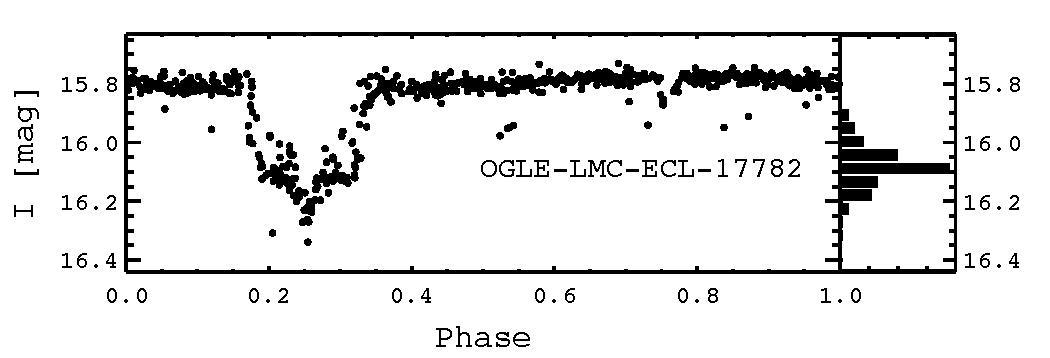
\includegraphics[width=0.98\textwidth,trim={0.0in 0.2in 0 0}]{figures/chapter3/f9_lmc11782.pdf}
\caption[与图 \ref{fig:lmc02192} 相同,但为系统 OGLE-LMC-ECL-17782($P=13.353\,\tif{d}$)。此系统为前人已识别的掩食盘候选体。由于该系统的掩食内星等分布同样拥有平台阶段,因而斜度与峰度值接近系统 OGLE LMC-ECL-11893($S=0.12$,$K=0.89$)。可以从图中看到该系统拥有变化的掩食轮廓和深度。]{与图 \ref{fig:lmc02192} 相同,但为系统 OGLE-LMC-ECL-17782($P=13.353\,\tif{d}$)。此系统为前人已识别的掩食盘候选体\cite{Graczyk2011}。由于该系统的掩食内星等分布同样拥有平台阶段,因而斜度与峰度值接近系统 OGLE LMC-ECL-11893($S=0.12$,$K=0.89$)。可以从图中看到该系统拥有变化的掩食轮廓和深度。}
\label{fig:lmc11782}
\end{figure}


需要说明的是,峰度斜度的筛选法并不能区分出以往类似 EE Cep 的进出掩食不对称结构,同样对诸如$
\epsilon$ Aur 的“W 型”掩食结构也没办法分离与识别,因为峰度斜度只能用来描述掩食内观测点的不均匀
性。从图 \ref{fig:lmcks} 中,还有另外一个系统 OGLE-LMC-ECL-17138 也在前面提到的实线方框(即掩
食盘可能区域)内。该系统的光变曲线以及掩食内星等统计如图 \ref{fig:lmc17138},似乎该系统并未显示
盘状掩食结构,那么为什么它的统计多极矩计算值和两个候选体类似呢?这里,我们将此峰度归结于这颗
系统存在掩食深度变化(Eclipsing Depth Variation,简称 EDV)。当我们在该系统单个周期内检查光变
曲线时,发现它的掩食内是明显的方波形状(峰度较小)。然而在周期折叠后的光变图中,该系统不同掩
食深度叠加后的确会成为该方法的例外,因而我们通过眼睛查看确认后将该系统排除出掩食盘候选体。

\begin{figure}[t]
\centering
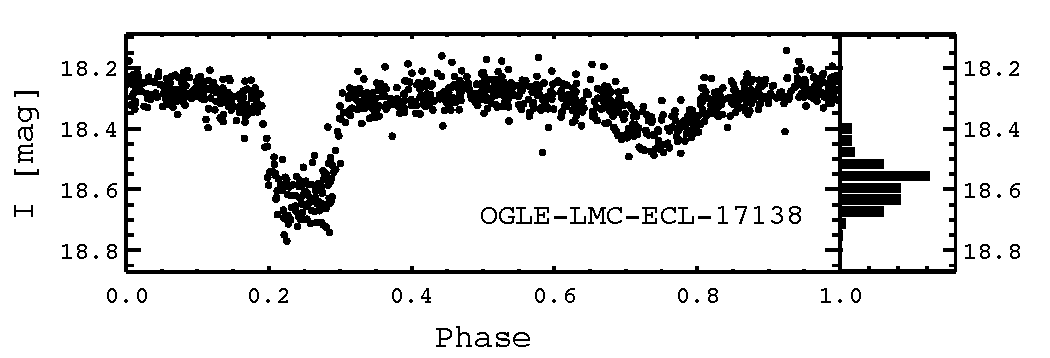
\includegraphics[width=0.98\textwidth,trim={0.0in 0.2in 0 0}]{figures/chapter3/f10_lmc17138.pdf}
\caption{与图 \ref{fig:lmc02192} 相同,但为系统OGLE LMC-ECL-17138($P = 11.1 \tif{d}$)。它是在 图 \ref{fig:lmcks} 实线框中的唯一的污染源。此系统拥有与掩食盘候选体 OGLE-LMC-ECL-11893 与 OGLE-LMC-ECL-17782 类似的掩食内星等分布斜度与峰度统计值($S=-0.36$ and $K=-0.02$),这是由系统的掩食深度变化所导致的。}
\label{fig:lmc17138}
\end{figure}


接下来,我们将该方法流程应用到 OGLE-III LMC EBs 次掩食,SMC EBs 主、次掩食以及 GD EBs 样本
中。在 LMC EBs 样本中,我们运用同样的方法总共找到 418 个高信噪比次掩食系统,然而在这些系统中
并没有找到掩食盘的候选体。而对与 SMC 中 EBs 样本,我们将 6,138 个系统缩小至 748 个高信噪比主
掩食,同样计算出斜度和峰度分布图并分析后我们得到了一个疑似掩食盘系统 OGLE- SMC-ECL-0007,
由于该双星周期为 $1.211 \tif{d}$ 并且主次掩食都发现了同样的非对称结构,因此猜测两颗星同时拥有掩
食盘的概率应该不会大。与此同时,文献 \citen{Pawlak2013} 的研究显示该系统为视线方向上的前景晚型
恒星,单独查看周期发现光变曲线在掩食内仅拥有 3---4 个测光点,因此我们怀疑该双星有 ETV 或者存在
星风,但也并不能对该系统下定论。

\begin{figure}[t]
\centering
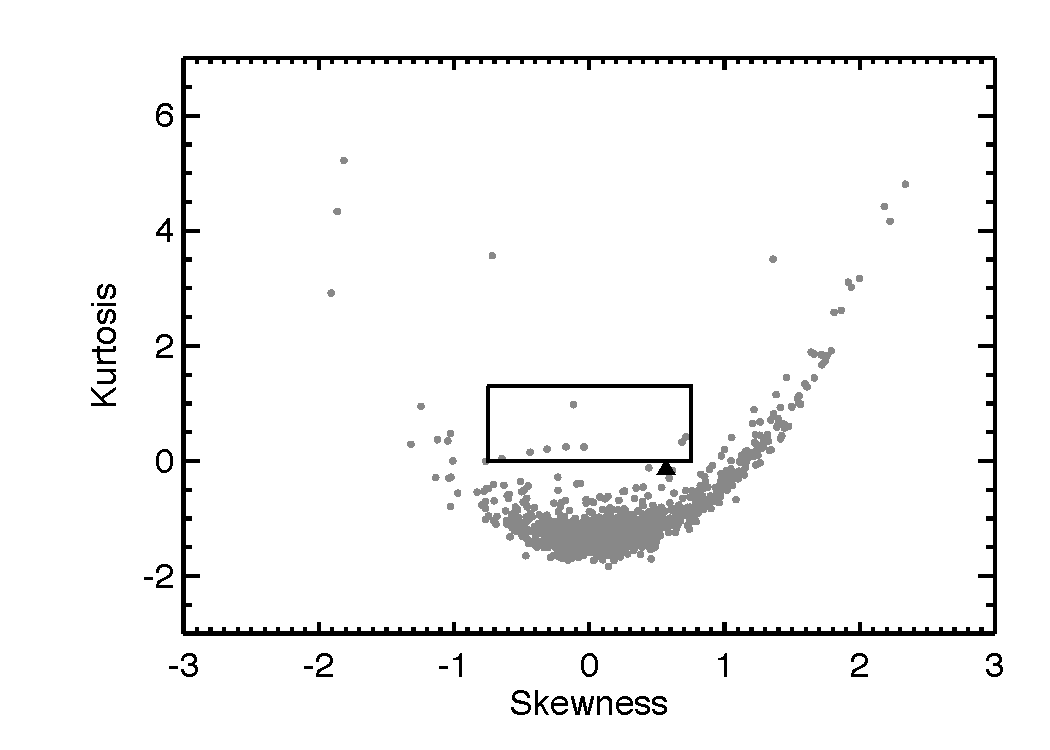
\includegraphics[width=0.98\textwidth,trim={0.4in 0.2in 0 0}]{figures/chapter3/f11_smcks.pdf}
\caption{与图 \ref{fig:lmcks} 相同,此图样本为 SMC EBs。我们同样检验了掩食盘在斜度峰度图上的可能区域,发现所有的点几乎都没有任何掩食盘的迹象,除了用三角形标注的系统 OGLE-SMC-ECL-0007(参见图 \ref{fig:smc0007})。虽然该系统在实线方框之外,光变曲线掩食内部分有些微的不对称性。}
\label{fig:smcks}
\end{figure}


\begin{figure}[t]
\centering
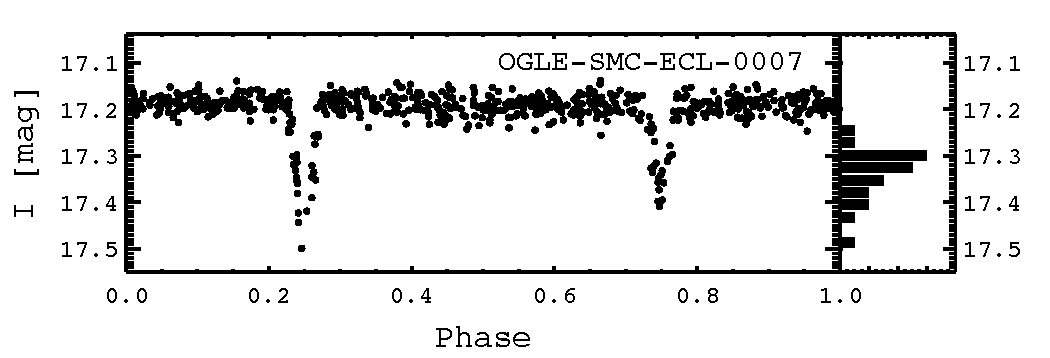
\includegraphics[width=0.98\textwidth,trim={0.0in 0.2in 0 0}]{figures/chapter3/f12_smc0007.pdf}
\caption{与图 \ref{fig:lmc02192} 相同,但为系统 OGLE-SMC-ECL-0007($P = 1.211 \tif{d}$)。此系统为 SMC EBs 中可能的掩食盘例子。它掩食内星等分布统计显示出不对成性$S=0.57$ and $K=-0.15$)。可以看出来主掩和次掩都为不对称结构,应为该系统为短周期双星,因此我们怀疑它同样存在 ETV。}
\label{fig:smc0007}
\end{figure}

最后,前文提到的方法被应用到 GD EBs 样本中,同样未发现明显的掩食盘信号(共 570 个高信噪比系
统)。这可能是因为 GD 样本的掩食深度噪声比相对于 LMC 甚至 SMC 都要差一些,并且在 GD 样本中
大部分恒星都偏年老,而盘的年龄要远远小于恒星的年龄。需要说明的是,在 GD EBs 样本中,最长周期
仅为 $P = 103.502 $天,在掩食盘搜索工作中,双星的间距越大,那么它们周围盘的洛希半径也就越
大,充满洛希半径的盘也更容易被巡天发现(关于洛希瓣请参考附录图 \ref{fig:rocher}。)。

\subsection{LMC 中掩食盘候选体的性质} \label{sec:discebprop}

文献 \cite{Derekas2007,Graczyk2011} 中提到 LMC 中 EBs 的色指数星等分布图具有双峰结构,分别为偏蓝
的近主序星和偏红的红巨星、超巨星(参见 \S \ref{apdx:HRdiagram},图 \ref{fig:hrdiagram})。那么在 
OGLE-III 的 EBs 中有多少为主序星呢?如果在这里我们定义$V - I \le 0.5 $ mag 为主序,那么在这 2823 
个高信噪比的 LMC EBs 中,一共有 2,471 对在主序附近。


我们将所有高信噪比 LMC EBs 的色指数 --- 星等画在图 \ref{fig:lmctracks} 中,可以看到 OGLE-LMC-ECL- 
17782(实心方框)和 OGLE-LMC-ECL-11893(实心三角)拥有接近与主序性质。此图采用文献 
\citen{Marigo2008} 提供的 Pandova internet server\footnote{\url{http://stev.oapd.inaf.it/cgi-bin/cmd}} 来制作
金属丰度为 $Z=0.006$(LMC 的经典丰度值)年龄跨越 $\log_{10}$(age/yr)$=6.0-9.0$ 且步长为 $\Delta 
\log_{10}$(age)$=0.1$ 的颜色---星等图。图中我们保留原始的 LMC EB 样本的星等与色指数值不变,而是将等年
龄线做了消光红移修正。修正量为 $A_V=0.55$(文献\citen{Zaritsky2004}),距离模数为 $\delta m=18.48$ mag 
(\citen{Walker2012})。下面我们将详细分析这两个系统。


\begin{figure}[t]
\centering
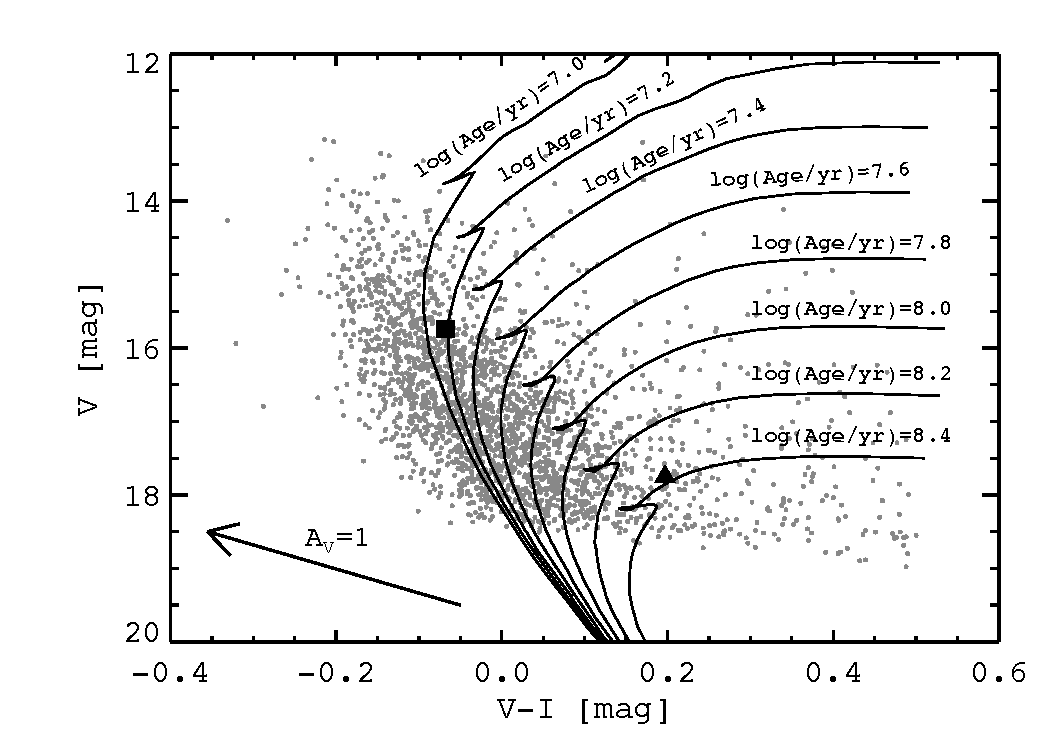
\includegraphics[width=1.0\textwidth]{figures/chapter3/f13_isotracks.pdf}
\caption[ LMC 低噪声 EB 样本的颜色 --- 星等分布图,其中 $V - I \le 0.5 $ mag 定义为主序系统。那么前文提到的掩食盘候选系统 OGLE-LMC-ECL- 17782(实心方框)和 OGLE-LMC-ECL-11893(实心三角)的多波段测光性质与主序正好吻合。叠加在其上的曲线为主序星从 $\log_{10}$(age/yr)$=7.0-8.4$ 步长为 $\Delta \log_{10}$(age)$=0.2$ 的等年龄线(Marigo et al. 2008)。并且这些等年龄线的红化已经通过 0.55 星等的消光与 18.48 星等的距离模数修正过,另外图中的箭头为 $A_{V}=1\,\rm{mag}$ 的消光矢量。]{ LMC 低噪声 EB 样本的色指数 --- 星等分布图,其中 $V - I \le 0.5 $ mag 定义为主序系统。那么前文提到的掩食盘候选系统 OGLE-LMC-ECL- 17782(实心方框)和 OGLE-LMC-ECL-11893(实心三角)的多波段测光性质与主序正好吻合。叠加在其上的曲线为主序星从 $\log_{10}$(age/yr)$=7.0-8.4$ 步长为 $\Delta \log_{10}$(age)$=0.2$ 的等年龄线\cite{Marigo2008}。并且这些等年龄线的红化已经通过 0.55 星等的消光与 18.48 星等的距离模数修正过,另外图中的箭头为 $A_{V}=1\,\rm{mag}$ 的消光矢量。}
\label{fig:lmctracks}
\end{figure}


\subsubsection{OGLE-LMC-ECL-17782} \label{sec:lmc17782}

对于 OGLE-LMC-ECL-17782 系统,我们将现有的测光信息汇总于表格 \ref{tbl:photo17782}。然而文献 
\citen{Zaritsky2004} 与 文献 \citen{Massey2002} 二者观测的星等与颜色并不相符,因此很难直接限定这个系统的
年龄。这也许是由于观测时间正好相互不重叠导致的。文献 \citen{Massey2002} 中的观测一共包括在 Cerro Tololo 
Inter-American Observatory(稍早于 \textsc{UT} 时间)观测的五个夜晚,\textsc{UT} 1999 年 1 月 8 日,
\textsc{UT} 2001 年 3 月 28--30 日与 UT 2001 年4 月 1 日。通过文献 \citen{Graczyk2011} 提供给的星历表,可
知该系统周期为 13.352899 天,主掩极小值开始于 Heliocentric Julian Date(HJD)2453563.2912,因而掩食可
能发生在  \textsc{UT} 1999 年 1 月 7 日 23 小时或者 \textsc{UT} 2011 年 4 月 1 日中午时刻,故文献 
\citen{Massey2002}  中给出的观测时间很可能落在主掩食内(文献 \citen{Zaritsky2004} 并未给出他们的观测时
间)。然而掩食内此系统会明显偏暗(星等值会变大),因而文献 \citen{Massey2002} 与文献 
\citen{Zaritsky2004} (与文献 \citen{Derekas2007} 以及文献 \citen{Ulaczyk2012} 一致)拥有不相符的 UBV 波段
星等并不能认为是盘遮挡住主星的原因,但也不能排除盘在文献 \citen{Massey2002} 观测的时间内遮挡伴星的量
少了一些。OGLE-III 的观测显示该系统并没有明显的掩食外亮度变化。值得一提的是,文献 \citen{Rivinius2013} 
曾提到一些 B 型恒亮度的确会偶尔突然增大,这背后的机制也还有待解释。


虽然 UBV 波段的星等稍有争议,但在 I 波段以及红外波段观测却出奇的一致。该系统主掩与次掩的时间间隔为 
0.5 个相位,因此轨道有很大几率为圆形的。同时掩食最深处的光变曲线形状为尖角形预示着主星与伴星拥有相近的半径
大小(伴星半径大于主星 2 倍以上,稍稍有观测倾角的很少数情况也可能造成类似的掩食形状)。为了更好的该星
的物理性质,本文使用 \textsc{NIGHTFALL} 程序\footnote{更多信息请参见 Nightfall 用户手册\cite{Wichmann2011},链接
\url{http://www.hs.uni-hamburg.de/DE/Ins/ Per/Wichmann/Nightfall.html},该程序考虑了临边昏暗、引力昏暗(增
量)以及恒星等势面形状等因素。}来拟合该系统的光变曲线。我们的模型内包含三个组分:主星、伴星以及星周
盘,并通过手动调整参数来使得恒星的物理参数最好的拟合光变曲线。

{\renewcommand{\arraystretch}{1.3}
\begin{table}[t]
\caption{OGLE-LMC-ECL-17782 系统宽带测光信息表}
\label{tbl:photo17782}
\centering
\begin{tabularx}{0.9\textwidth}{@{\extracolsep{\fill}}c l c l c}
\hline
波段  & 星等  & 参考文献 & 星等 & 参考文献 \\
\hline
$U$  & $15.356\pm 0.027$  & Z04 & 14.38 & M02\\
$B$ & $15.563\pm 0.062$ & Z04 & 15.13 & M02\\
$V$ & $15.711\pm 0.027$ & Z04 & 15.784 & U12\\
$V$ & 15.793                    & D07 & 15.21 & M02 \\
$V$ & 15.737                    & G11 &  15.793 & D07      \\
$R$ & 15.888                   & D07    &          &         \\
$I$ & $15.855\pm 0.035$ & Z04 & 15.895 & U12 \\
$I$ &   15.805                   & G11 &              & \\
$J$  & $15.97 \pm 0.02$   &   K07 & $15.913\pm 0.039$ & C06 \\
$H$  & $15.98\pm 0.02$    &   K07  &$15.916\pm 0.074$ &C06 \\
$K_{_{\rm{S}}}$ & $15.92\pm 0.07 $  & K07 & $15.907\pm 0.137$ & C06 \\
$\left[3.6\right]$ &  $ 15.951 \pm  0.076$ & M06 & &\\
$\left[4.5\right]$ & $15.853  \pm   0.088$ & M06 && \\
\hline
\end{tabularx}
\medskip \\
此表格使用的测光值引自参考文献列表如下:
Z04 --- 文献\citen{Zaritsky2004};
K07 --- 文献\citen{Kato2007};
M06 ---  文献\citen{Meixner2006};
C06 ---  文献\citen{Cutri2012};
U12 ---  文献\citen{Ulaczyk2012};
M02 ---  文献\citen{Massey2002};
G11 --- 文献\citen{Graczyk2011};
D07 ---  文献\citen{Derekas2007}。
\end{table}
}

拟合的结果展示在图 \ref{fig:discfit} 中,拟合过程中我们发现即使假设盘已经完全延展到伴星的洛希瓣,伴星的质
量都几乎必须得和主星差不多大($M_2 \gtrsim 0.8 M_1$)才能比较好的拟合光变曲线主掩最大值两侧的宽翼部
分。考虑到 Nightfall 并不能调整盘的不透明度参数,因此我们假设盘为纯粹的黑体辐射,并且通过调整盘的轨道倾
角以及几何厚度来更好的符合主掩食极大两侧的宽翼部分。根据图 \ref{fig:lmctracks} 给出的该系统的绝对 V 波段
视星等(即亮星亮度之和)以及统一幅图中得到的初始输入有效温度与大体质量(假设两颗星年龄相同),我们将 
OGLE-LMC-ECL-17782 系统的物理参数限定在有效温度约 29 000 K,光度为 $1.4 \times 10^4 L_\odot$ 匹配的总
质量为 14.3 $M_\odot$,年龄 50 万年,消光大约为 $A_V \sim 0.4$ 星等。考虑到主星和伴星的总光度,可得到系
统经过消光修正后的绝对星等 $M_V$ 为 $-3.1$。 从而可以计算得到 $U-B = -0.92$ 星等,$V-I = -0.12$ 星等。该
值与表格 \ref{tbl:photo17782} 中所列的文献 \citen{Zaritsky2004} 以及文献 \citen{Ulaczyk2012} 相符合。这里
拟合得到的消光值比文献 \citen{Zaritsky2004}估算的平均消光值稍微偏小,如果消光值比拟合值偏大那么 $V-I$ 色
指数久无法很好的匹配上文献中给出的值;相反如果消光减小至 0.3 星等,主星的年龄会明显的增加(为了拟合系
统的光度),从而掩食的时长将会明显大于观测值。

\begin{figure}[t]
\centering
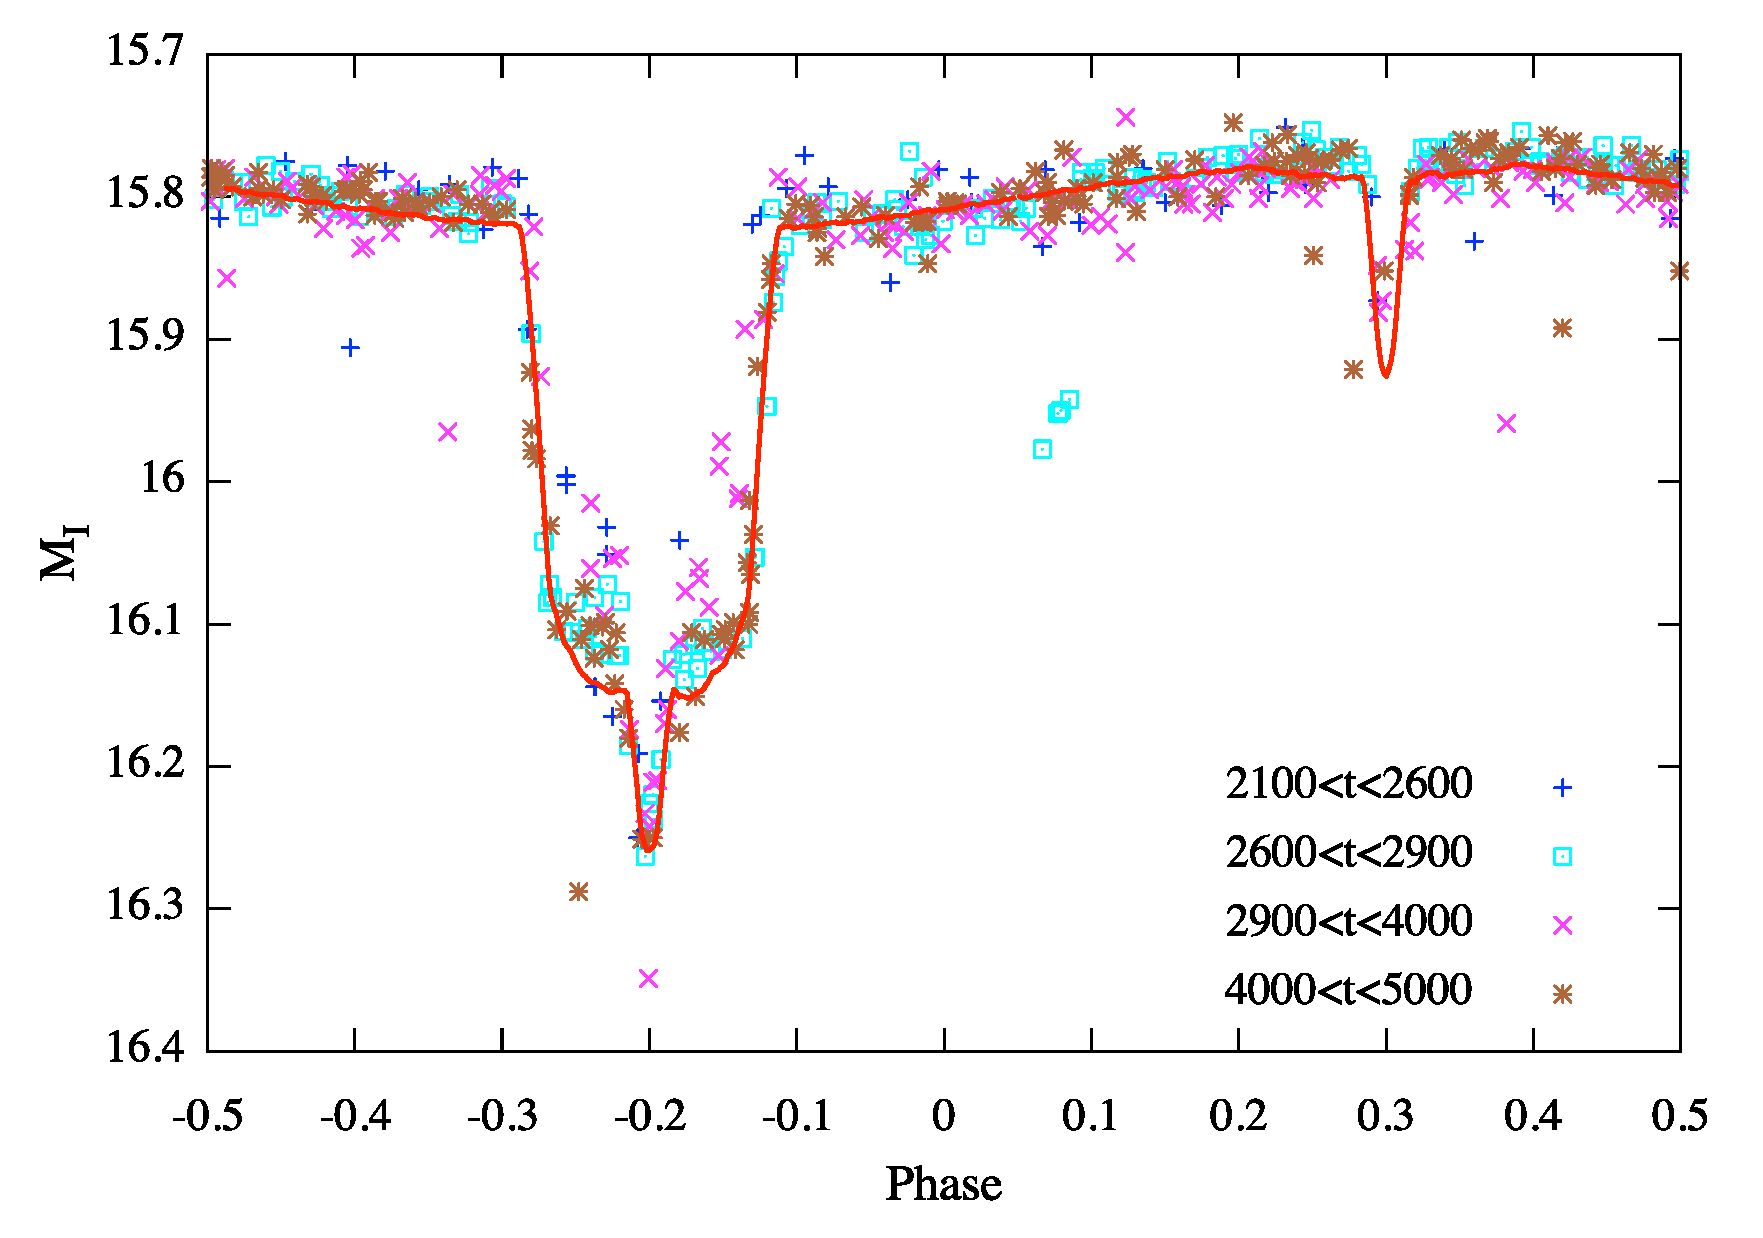
\includegraphics[width=1.0\textwidth]{figures/chapter3/f14_discparam.pdf}
\caption{周期叠加后的 OGLE-III 系统 OGLE-LMC-ECL-17782 以及拟合的光变曲线图。不同点代表不同的时间测得的数据,图中的时间定义为 $t = \tif{HJD} − 245 0000$。关于此  Nightfall  程序的拟合参数请参见表格 \ref{tbl:discparam}。为了显示,我们将此图主掩极大的相位移动了 $\theta_\tif{p}= -0.2$。}
\label{fig:discfit}
\end{figure}

该系统的除了主掩食有浅一些的盘掩食迹象,次掩食也同样可以看到类似的结构,拟合程序 Nightfall 看似并未考虑
次掩时盘对主星的反射,但次掩两侧的长时间浅侧翼也似乎是该反照效应。我们考虑了该系统中正弦相位导致的亮
度变化(振幅大小为 0.025 星等),这正是由于伴星在不同轨道相位上的反射光导致的。同时为了检测该伴星究竟
是否为致密星,我们通过 XMM-Newton 的 LMC 曝光照确认 X-rays 流量为否定的结果。

{\renewcommand{\arraystretch}{1.4}
\begin{table}
\caption{OGLE-LMC-ECL-17782 系统的光变曲线拟合参数}
\label{tbl:discparam}
\centering
\begin{tabularx}{0.9\textwidth}{@{\extracolsep{\fill}}lr}
\hline
Orbital Period & 13.3525 days \\
Primary $T_\tif{eff}$  & 29,000  K  \\
Secondary $T_\tif{eff}$  & 25,500 K   \\
Disk $T_\tif{eff}$  & 6000 K  \\
Primary Roche Fill & 0.176\\
Secondary Roche Fill & 0.158\\
Disk  Roche Fill & 0.97 \\
Orbit Inclination & 87.5$^\circ$ \\
Orbital eccentricity & 0.0 \\
Disk aspect ratio $H/R$  & 0.03 \\
Mass ratio $M_2/M_1$ & 0.8 \\
Primary mass $M_1$     &  $14.3 M_\odot$ \\
Total mass  & $26 M_\odot$ \\
Primary Radius  & $4.6 R_\odot$ \\
Secondary Radius & $3.7 R_\odot$ \\
Disk Radius  & 32.6 $R_\odot$, 0.15 AU \\
Semi-major axis & 70.0 $R_\odot$, 0.33 AU \\
Primary Luminosity & $1.3 \times 10^4 L_\odot $\\ 
Secondary Luminosity & $5000 L_\odot $\\ 
\hline
\end{tabularx}
\medskip \\
对 OGLE-LMC-ECL-17782 系统主星、伴星以及掩食盘的 Nightfall 拟合物理量表格(光变曲线拟合见图 \ref{fig:discfit})。
\end{table}
}

如果该掩食盘在主掩时彻底遮挡住主星,那么通过该掩食深度可以估算得到该盘的光深大概为 $\tau \sim 0.3$。而
部分盘遮挡住主星的情况将会对应更大的光深。通过恒星的总质量(26$\tif{M}_\odot$)我们同样可以估算该盘的
大小为 $\sim 0.15\tif{AU}$。这时考虑到主星的光度($\sim  1.3\times 10^4\,\rm{L_\odot}$),盘吸收了主星 30\% 
的光子能量后,对应于在 0.33 AU 处的温度至少为 $\sim 5500\,\tif{K}$(尚未考虑伴星的辐射)。如果通过盘在整
个掩食周期上所花的时间,则对应与不到 10\% 的遮挡横截面。不管如何,这样的吸收在 Be 恒星周围都很有可能
造成红外超\cite{Waters1988,Dougherty1994}。而温度高达 5500 K 的盘已经完全可以升华所有的盘内固体物质
(即使光变曲线形状更接近于弥散的尘埃盘)。而在如此高的盘遮挡面积下,根据盘的大小以及温度和掩食深度,
不透明度的来源极有可能为 Thompson 散射,以及自由---束缚辐射(如 H\textsc{I} 的光致电离)而不是自由---自由
辐射\cite{Rivinius2013}。而这里我们得到的光变曲线拟合模型并不能很好的限制此系统的性质是因为没有视向曲线
的测量(包括光谱型以及发射谱)。

\subsubsection{OGLE-LMC-ECL-11893} \label{sec:lmc11893}

正如文献 \citen{Scott2014} 中讨论到的,OGLE-LMC-ECL-11893 的光谱显示系统的主星光谱型为 B9III。该系统的
光谱显示主星刚离开主序阶段,也拥有稍稍大于 LMC EB 系统的平均消光。该系统的年龄大约为 150 Myr,消光以
及绝对 V 波段星等,对于光谱型 B9 的恒星而言,该星的绝对光度比主序星阶段常见值明显大一些。虽然该系统双
星的周期为 468 天,但主星的温度非常高,因而星周盘的温度也很可能超过固体升华点。关于该系统的具体讨论以
及掩食盘的详细拟合请参见文献 \citen{Scott2014}。


\section{掩食盘概率估算} \label{sec:discebdiscuz}

与以往 OGLE-II 巡天\cite{Wyrzykowski2003}相比,OGLE-III LMC 巡天的观测时间几乎整整多了一倍,而且归功于
测光精度的提升,OGLE-III LMC 发现的 EBs 数目也比以往多出了一倍。根据文献 \citen{Graczyk2011},LMC EB 
样本星表的完备度几乎达到 90\%(对于 $i$ 波段视星等亮于 18 等的子样本完备度还会更高)。由于 OGLE-III 
LMC 高可信的完备度,我们在这边讨论 LMC EB 样本探测掩食盘的完备度问题。

从文献 \citen{Haisch2001} 中可知,银河系内年轻恒星团的盘出现概率与年龄成反相关性,而且早型恒星盘的寿命
也会明显短过晚型星族,如不足 10\% 的 A-F 型恒星在 3 Myr 年龄内拥有盘,而 T-Tauri 恒星却可高达 30--35\%
\cite{Hernandez2007}。另外年轻恒星是否拥有盘以及盘存活的时间也依赖于恒星的是否处于多星系统中。在对 
1--2 Myr 年龄的 Taurus-Auriga 恒星形成区的搜寻中,Harris 等人发现多星系统的恒星仅有三分之一的比例拥有能
够被探测到星周尘埃盘的毫米波段辐射($\gtrsim$ 10 mJy),与之相比的单星系统却有三分之二的比例
\cite{Harris2012}。考虑到这些因素,我们保守估算在年龄不到 1Myr 的早型星样本中,大概只有 5\% 左右的双星
能够拥有星周盘,而对于 10 Myr 的系统比例则会下降到 1/10。

正是由于这些系统中星周盘存活时标相对较短,因而才会在 LMC 的样本中看到拥有星周盘的双星系统候选体仍处
于主序阶段(当然盘也可能通过后期的质量交换而形成)。在我们分析筛选得到的 2,471 个高信噪比早型 EB 系统
中,至少应该有两个可能的掩食盘候选体(两个通过掩食中平台而发现的盘,如果通过查找 W 型或者不对称型的
掩食内光变曲线还可以找到类似 $\epsilon$ Aur 和 EE Cep 的系统)。如此我们得到的概率 $\gtrsim 1/1000$,应
该和前人在 EBs 中找到盘的比例没有明显的不一致性。然而这里,我们搜索到的两个掩食盘候选体 OGLE-LMC-
ECL-11893 以及 OGLE-LMC-ECL-17782 都应该不是原初恒星盘。可能是由于恒星星风作用\cite{Graczyk2011}或
者快速自转的恒星周围抛射出的喷射盘\cite{Rivinius2013}。相比于 OGLE-LMC-ECL-17782 系统 13.3 天的较短周
期,我们更秦翔宇在距离更远的双星周围找到类似的尘埃盘。

最后需要考虑的是,由于我们探测掩食盘的方法并不能有效的探测  W 型或者不对称型的掩食内光变曲线系统如 $
\epsilon$ Aur 和 EE Cep,因而这边估算的 LMC EB 样本中掩食盘的出现概率还会减少额外的 50\%。通过掩食中
平台的方法来探测 OGLE-LMC-ECL-17782 并不能适用于每个系统 OGLE-LMC-ECL- 11893,因此我们不推荐增加 
\ref{fig:lmcks} 图中的实线方框区域来包括更多的系统,或许更好的做法是利用其他的方法来探测掩食盘可能出现的
特殊形状。




\chapter{统计与性质} \label{chapter:data_stat}
%%%%%%%%%%%%%%%%%%%%%%%%%%%%%%%%%%%%%%%%%%%%%%%%%%%%%%%%%%%%%%%%%%%%%%%%%%%%%%%
% 学位论文的正文应以《结论》作为最后一章
\chapter{总结与展望} \label{chapter:conclusion}

\epigraph{... the ways by which men arrive at knowledge of the celestial things are hardly less wonderful than the nature of these things themselves}{\textit{Johannes Kepler}}


\section{更丰富细致的行星样本}

在短短二十年内,系外行星领域在仪器方面可谓发生了质的飞跃,新发现的系统也一次又一次地
打翻了以往我们对于行星陈旧的认知。可我们在系外行星这条探索之路上才刚刚启程,下一步科
学研究依旧得依赖更多与更深的挖掘。在仪器方面,传统的视向速度依然在稳步中不断提高仪器
的谱分辨率与可靠度(如 TESS\cite{Ricker2015} 与 PLATO\cite{Rauer2014})以尝试去发现更
多的中长周期行星,这包括温木星(warm Jupiter)以及更长周期的冷木星。其中对温木星的探
测与刻画是通往解释它们自身以及热木星形成的必经之路
\cite{Petrovich2016,Huang2016,Dong2014a,Frewen2016,Dawson2014a,Antonini2016}。
在目前形成热木星的机制中,盘迁移能够解释低偏心率以及处于共振的系统,偏心率较中等的系
统则往往只能通过行星---行星散射形成,而更高偏心率的则很可能正处于强烈的潮汐圆化过程。
如何区分不同的机制以及温木星究竟是不是失败的热木星,都是非常值得探究的问题。这群特殊
的木星在解开行星形成密钥的同时,也对恒星的演化有着重要的暗示,具体请见 \S \ref{sec:fateofplanets})。

再者,利用已知行星系统去寻找发现质量更小的超级行星也十分有趣。类似 WASP-47 这样的系统
在观测中又究竟还有多少遗漏,而小质量行星的信号到底会不会被掩埋在已存在巨行星的 RV 信号
中呢?这些问题必须得利用多观测手段同时查漏来解答,比如 \textit{Gaia} 卫星的天体测量数据可
用来解除拟合参数中轨道倾角 $i$ 与真实质量的简并\cite{Gaia2016},并且在探测一些处于共振的
行星系统也有独特的优势\cite{Wu2016}。

相比之下,凌星法在探测系外行星的密度,表层大气环流以及压强温度垂直分布轮廓有着独特的先
机(如图 \ref{fig:transitspectro}),直接成像法亦可直接测量行星的光谱。如今这部分系统只有三十
颗行星成功利用 \textit{Spitzer} 与 Hubble 观测到其高层大气结构和垂直温度分布,如系统 HD 189733 b
\cite{Knutson2007}。利用凌星发测得的行星半径与 RV 得到的质量还可以初步限定行星的密度(如
图 \ref{fig:massrad})。对诸多天体研究\cite{Baraffe2008,Fortney2007}显示从恒星级天体到类地行
星,质量与半径的关系呈现出截然不同的指数系数:

\begin{equation} \label{eq:massrad}
R \propto \left\{
  \begin{array}{lr}
       \,   M            &  \qquad \text{恒星} 	   \\
       \,   M^{-1/8}  &  \qquad \text{褐矮星} 	   \\
       \,   M^{1/10} &  \qquad \text{气巨行星}   \\
       \,   M^{1/3}   &  \qquad \text{类地行星} 
  \end{array}
\right.
\end{equation} \myequation{不同天体的质量半径关系}

这些关系恰恰可以反映行星内部的成分以及物态方程\cite{Zapolsky1969}。同样的,超级地球中大
气与固体组成构造的差别也将能很好的解释类似超级地球等「过渡型」行星究竟是失败的气巨星还
是大个头的地球\cite{Rogers2015a,Lissauer2014},这也能帮助我们了解超级地球在原行星盘中的
形成地点和演化吸积过程\cite{Miguel2011,Haghighipour2013}。

\begin{figure}[t]
\centering
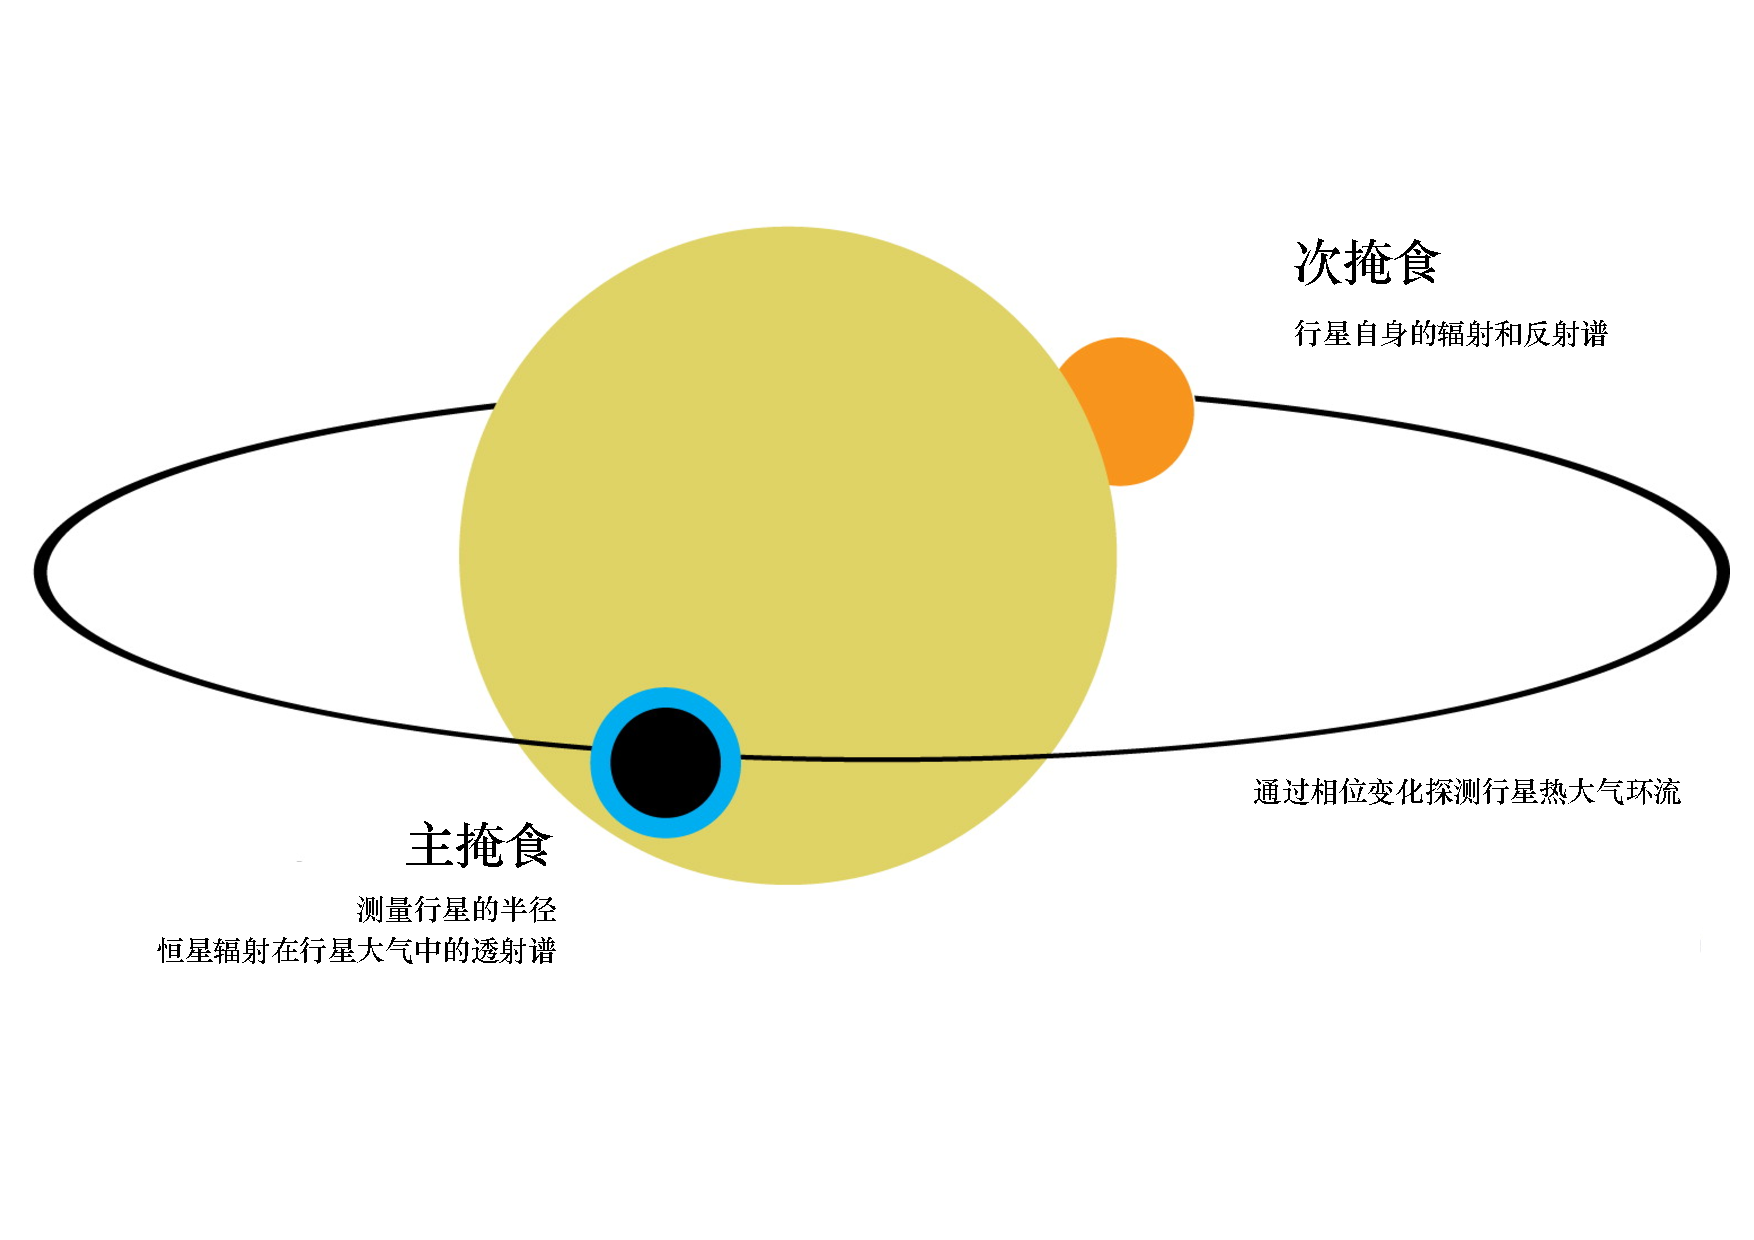
\includegraphics[width=1.0\textwidth]{figures/chapter5/fig1_eclipsing.pdf}
\caption{凌星探测法对行星物理性质的后续观测示意图。从主掩食(Transit)到次掩食(Occultation)可以分别看到行星大气随着相位变化以及行星大气所蕴含的半径和大气成分等重要信息。图片版权 Sara Seager。}
\label{fig:transitspectro}
\end{figure}


除了研究这些特殊的行星之外,另一个更重要的目标就是将行星质量探测下限延伸至类地行星甚至
系外卫星。目前系外卫星探测率至今仍为零\cite{Kipping2011},而在探测极限允许的条件下,这很
可能与主星的光致蒸发与动力学作用相关\cite{Yang2016}。而在 HEC 列表
\footnote{\url{http://phl.upr.edu/projects/habitable-exoplanets-catalog}}中,总共也列出约 50 颗的潜
在宜居住行星(habitable exoplanets),我们究竟该如何定义宜居性\cite{Kasting1993},而宜居性
又是否与行星本身的质量、温度、大气与液态水、其他行星以及主星的活动之间(尤其是 M 型恒星)
有必然关联\cite{Kasting2003,Segura2005,Scalo2007}?另外系外生命的存在信号(即系外生物信号,
biosignature)以及她们是否真的依赖类似地球大气中的 $O_2$ 等等。这些问题或许都值得去等待
James Webb Space Telescope(JWST) 卫星的发射来揭晓。


\begin{figure}[t]
\centering
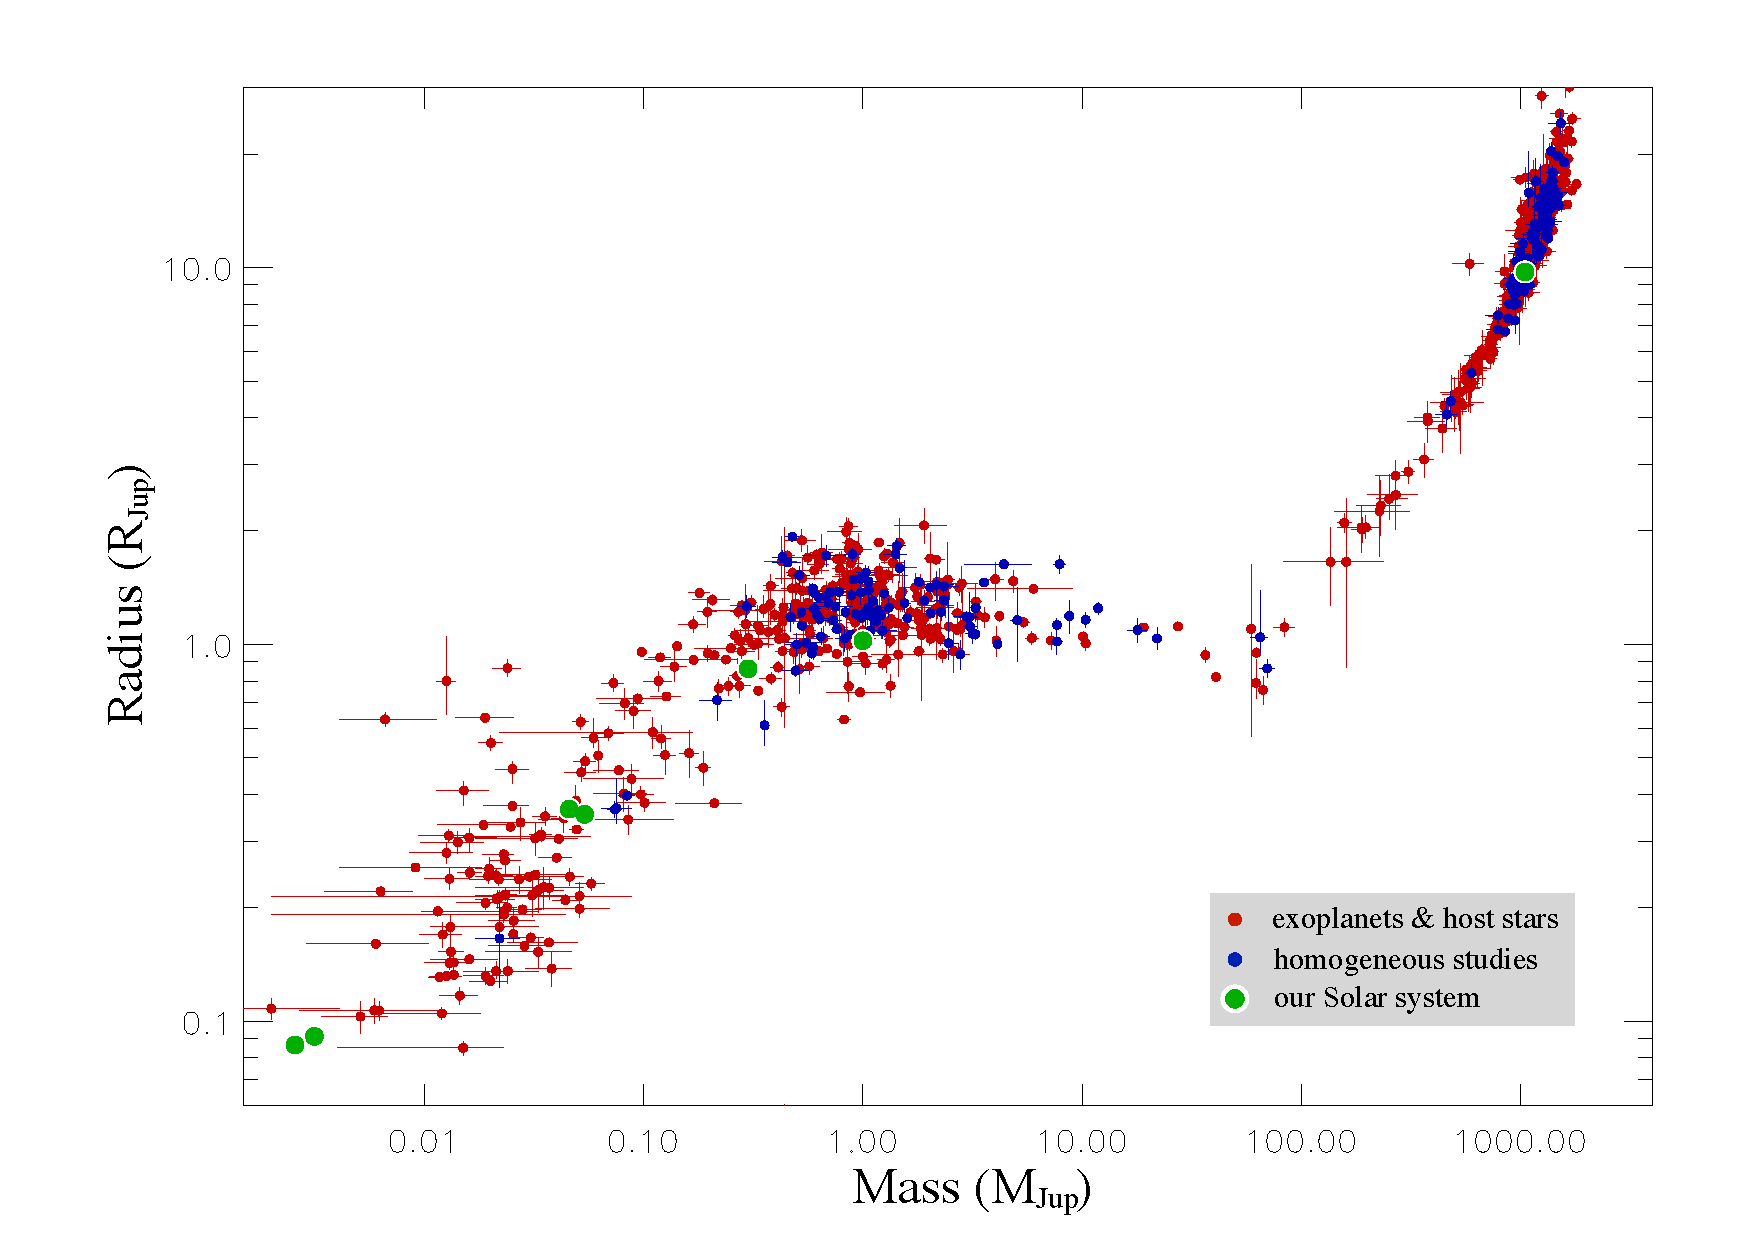
\includegraphics[width=1.0\textwidth]{figures/chapter5/fig2_massrad.pdf}
\caption{凌星法探测的行星的质量与半径关系图(包括其主星)。从恒星、矮星到气态巨行星与类地行星半径质量关系呈现处的不同变化向我们反映了它们内部结构与物质状态的不同。此图数据源自网站 TEPCat。}
\label{fig:massrad}
\end{figure}
 

\section{全局的行星系统演化} \label{sec:fateofplanets}

作为行星原材料的摇篮,恒星以及诞生恒星的分子云和周边的星际空间在支配恒星以及后续的行星
演化有着至关重要的作用。一些研究显示不同的质量以及金属丰富的主星会对其中行星出现的概率
和质量其决定性因素\cite{Fischer2005},比如 M 型矮星周围的气巨星形成率会偏低,而类地行星则
正好相反\cite{Johnson2007b,Cumming2008,Kennedy2008},而随着恒星质量的增加大质量行星出
现的概率也会偏大,比如对于巨星和亚巨星分支,这类恒星周围更容易看到大质量行星\cite{Johnson2007}。
但与此同时,巨星周围的短周期热木星出现的概率却又偏少(共 99 个系外行星处于巨星周围,其中
周期小于 10 天的却只有 2 颗\footnote{\url{https://www.lsw.uni-heidelberg.de/users/sreffert/giantplanets/giantplanets.php}})。
这很可能是因为主星半径膨胀后潮汐作用将行星吞噬后的演化结果\cite{Sato2008,LilloBox2016}。


此外,在双星或者多星系统环境中行星形成过程和对类地行星的影响也不可小觑\cite{Desidera2007}。
太阳系内木星与地球可以同时存活,可是在双星系统中(如图 \ref{fig:staraffp} 所示)情况却大有不同,
在三体不稳定模型下\cite{Marzari2007},由于混沌效应,行星产生的概率明显随着恒星的交汇次数以
及时间而减小,同样若行星系统中存在类似木星的长周期行星,那么将对内行星系统造成更强的摧毁
效应,而且散射至外围的行星也可能是环双星行星候选体的一种形成机制\cite{Gong2013}。


\begin{figure}[t!]
\centering
\begin{subfigure}[b]{.48\textwidth}
\captionsetup{width=0.9\textwidth}
\centering
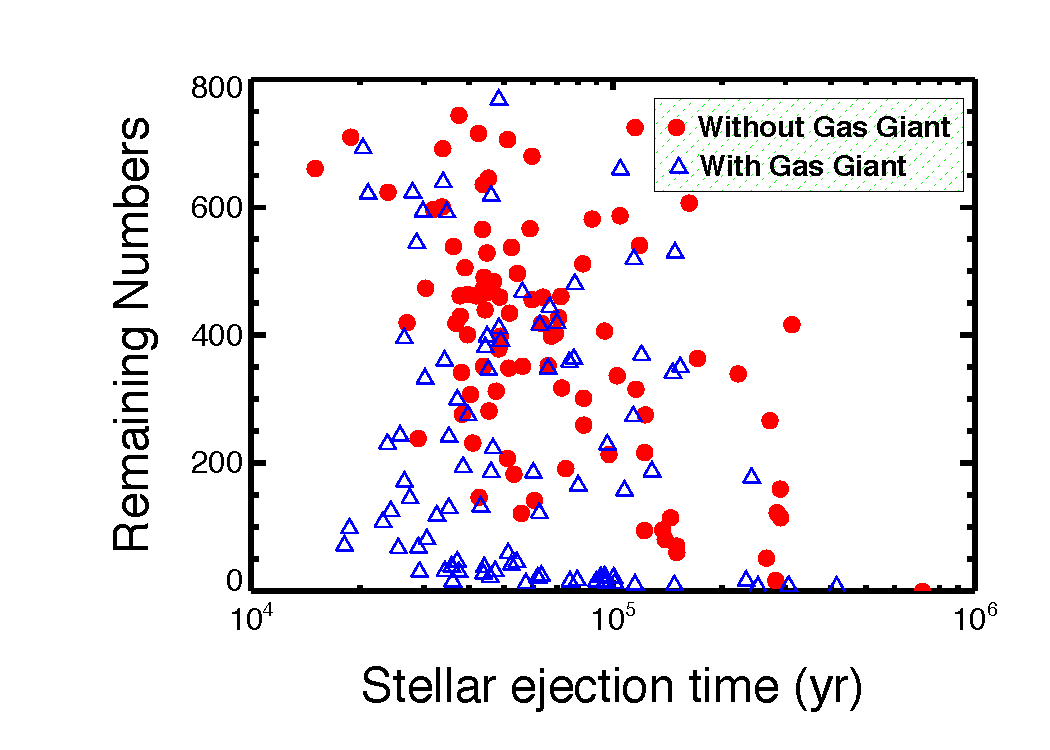
\includegraphics[width=0.95\textwidth]{figures/chapter5/fig3a_stellarenv.pdf}
\caption{恒星发生不稳定的时标对于行星系统内行星的存活率造成的影响。图中三角形表示质量为零的测试粒子(Testing Particle,TP)情况,而红色圆点则表示在系统中加入一颗木星质量的行星后木星的存活对 TPs 的影响。}
\end{subfigure}
\begin{subfigure}[b]{.48\textwidth}
\captionsetup{width=0.9\textwidth}
\centering
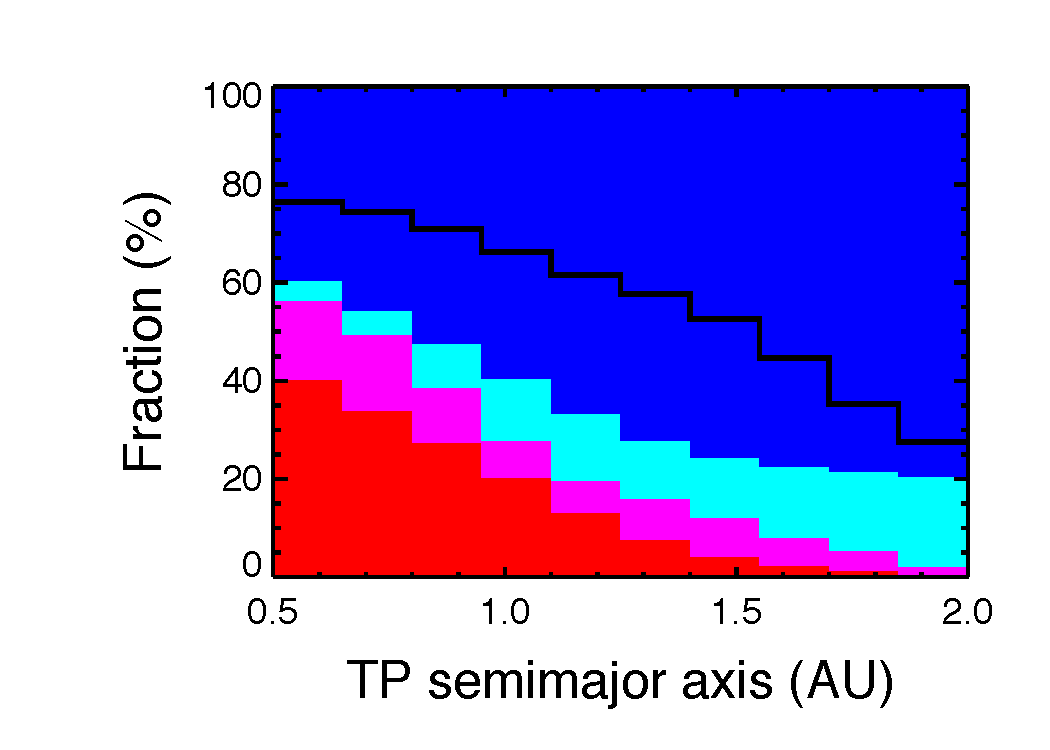
\includegraphics[width=0.95\textwidth]{figures/chapter5/fig3b_innerplanet.pdf}
\caption{在不同半长径下红色(气巨星逃逸, TPs 存活)、紫色(气巨星 TPs 均存活)、浅蓝色(气巨星存活, TPs 逃逸)与深蓝色(气巨星与 TPs 均逃逸 )的概率。黑色线则表示未添加气巨星,TPs 的存活比例。}
\end{subfigure}
\caption{恒星在多星系统中的形成环境对行星系统的影响:三星系统由于三体不稳定性会导致其中两颗恒星发生密近交汇,这种剧烈的动力学过程会导致行星系统发生不稳定性,此效应更会对恒星周围其他的行星如类地行星产生恶性连锁反应,因而气巨星对类地行星存在几乎是种灾难。}
\label{fig:staraffp} 
\end{figure}


随着恒星与行星系统的演化,灾难在所难免。比如在白矮星周围,光谱观测看到了其表面的重金属
污染\cite{Barstow2014},这样的污染很可能因为行星系统被潮汐撕裂后留下的残骸撞击中心致密性
导致的\cite{Vanderburg2015,Boyajian2016}。对于一些紧密间隔的行星系统,行星的不稳定时标大
大缩短\cite{Lissauer2011,Lovis2011,MacDonald2016},而就连太阳系内长期演化后都可能导致各大
行星之间的不稳定性发生,从而造成轨道交错以致最后彼此互相摧毁,化为碎屑\cite{Laskar1988,Laskar1990}。


\section{具现代化的范式转换}

当今的科学是一项重任,取之于民同时用之于民。全民参与以为着新的时代已经悄然到来(Citizen 
Science),其中 Zooniverse\footnote{\url{https://www.zooniverse.org}} 旗下的 Planet Hunters 已经
发表了十二篇文章,包括第一篇被认证的系外行星(参见文献 \citen{Schwamb2013} )。更多人提供
了额外能够让人们参与进来的提议,包括命名系外行星\footnote{\url{http://nameexoworlds.iau.org/}}
以及其它越来越丰富的可能性\cite{Hessman2010,Marshall2015}。在软件层面,整合源代码网站 
ASCL\footnote{\url{http://ascl.net/}} 以及越来越多建立在 Python 之上的开发工具也在极大程度上降低
了数据分析的门槛,如 Astropy \footnote{\url{http://www.astropy.org/}} 与 
Rebound\footnote{\url{https://github.com/hannorein/rebound}}。

另外利用机器学习(machine learning)分析以及深度挖掘数据(data mining)也将会在天文领域有
相应的一席之地\cite{Ball2010,McCauliff2015,Thompson2015}。若要结合大数据(big data)来反馈
到系外行星领域,星族合成方法(Population Synthesis )也许是最能够还原众多系外行星集体性质
与演化的途径之一\cite{Benz2014,Mordasini2009}。

\section{细致刻画单个系统}

热木星的大气环流

宜居性 Proxima Centauri

Kepler-78 b 等 USPs









%%%%%%%%%%%%%%%%%%%%%%%%%%%%%%%%%%%%%%%%%%%%%%%%%%%%%%%%%%%%%%%%%%%%%%%%%%%%%%%
% 致谢,应放在《结论》之后
\begin{acknowledgement}


\end{acknowledgement}

%%%%%%%%%%%%%%%%%%%%%%%%%%%%%%%%%%%%%%%%%%%%%%%%%%%%%%%%%%%%%%%%%%%%%%%%%%%%%%%
% 附录
\appendix
% 参考文献。应放在\backmatter之前。
% 推荐使用BibTeX,若不使用BibTeX时注释掉下面一句。
\nocite{*}
\bibliography{meldon_exoplanet}
% 附录,必须放在参考文献后,backmatter前
\appendix
%% Appendix tex file by Meldonization.

\chapter{文内常用约定} \label{apdx:nomenclature}
\section{物理符号含义} \label{apdx:symbol}
\begin{multicols}{2}
\begin{tabularx}{1.0\linewidth}{@{\extracolsep{\fill}}lr}
\centering
$a$      	     			&     轨道半长径 		\\
$d$      	     			&     质点二体间距离	 	\\
$P$      	     			&     轨道周期	 		\\
$e$      	     			&     轨道偏心率 		\\
$i$          	     			&     轨道倾角 			\\
%$\omega$      			&     近心点角距 		\\
%$\Omega$     			&     升交点经度 		\\
%$f$              			&     真近点角   			\\
$\tif{M}_\odot$          		&     太阳质量   			\\
$\tif{R}_\odot$          		&     太阳半径   			\\
$\tif{M}_\tif{J}$          		&     木星质量   			\\
$\tif{M}_\oplus$          	&     地球质量   			\\
$M_\tif{s}$          		&     恒星质量   			\\
$R_\tif{s}$          		&     恒星半径   			\\
$M_\tif{p}$         	 	&     行星质量   			\\
$m$         	 			&     视星等   			\\
$c$         	 			&     真空光速   			\\
$m$         	 			&     视星等   			\\
$\nu$         	 		&     光子频率   			\\
$k$         	 			&     玻尔兹曼常数   		\\
$h$         	 			&     普朗克常数   		\\
T		       	 		&      温度   			\\
$\tif{T}_\tif{p}$         	 	&      行星温度   		\\
$\tif{T}_\tif{s}$         	 	&      行星温度   		\\
$\tif{T}_\tif{d}$         	 	&      星周盘温度   		\\
$\tif{T}_\tif{eff}$         	 	&      有效温度   		\\

\end{tabularx}
\columnbreak

\begin{tabularx}{1.0\linewidth}{@{\extracolsep{\fill}}lr}
\centering
L		         	 	&      光度		   		\\
$\tif{L}_\tif{IR}$         	 	&      红外光度   		\\

\end{tabularx}
\end{multicols}

\newpage


\section{首字母缩写}  \label{apdx:acronym}
本文首字母缩写主要参考自书籍\citen{AstroDict},按照字母先后顺序排列如下:
\begin{multicols}{2}
\begin{tabularx}{1.0\linewidth}{@{\extracolsep{\fill}}lr}
\centering
AST3           &   南极巡天望远镜     	   	  \\  
BB		   &   黑体					   \\
CS 	 	   &   环恒星				   \\
CCD		   &   电荷耦合器件			   \\
CSTAR        &   南极之星望远镜阵列 		   \\  
EB               &   掩食双星 				   \\  
FFP             &   自由飘游行星        		   \\ 
FOV            &   视场			     		   \\ 
GB              &   银核球				   \\
GD              &   银盘				  	    \\
GI                &   引力不稳定              		    \\
IAU             &    国际天文学联合会   	    	    \\
IR               &   近红外波段		 	            \\
MMR           &   平运动共振   	                     \\   
MMSN         &   最小质量原行星盘                 \\
NIAOT         &   南京天文光学技术研究所       \\
NIR              &   近红外波段		             \\
OGLE         &    光学引力透镜实验   	     	     \\
PPD            &    原行星盘   	   	     	     \\
RV              &    视向速度                    	     \\
SED            &    光谱能量分布                   	     \\
TNO           &    海外天体                    	     \\
TTV            &    凌星计时变化             	     \\


\end{tabularx}
\columnbreak
\begin{tabularx}{1.0\linewidth}{@{\extracolsep{\fill}}lr}
\centering
YSO           &    初期恒星体                	     \\
\end{tabularx}
\end{multicols}




\chapter{二体运动示意图} \label{apdx:twobodyproblem}

\begin{figure}[h]
\centering
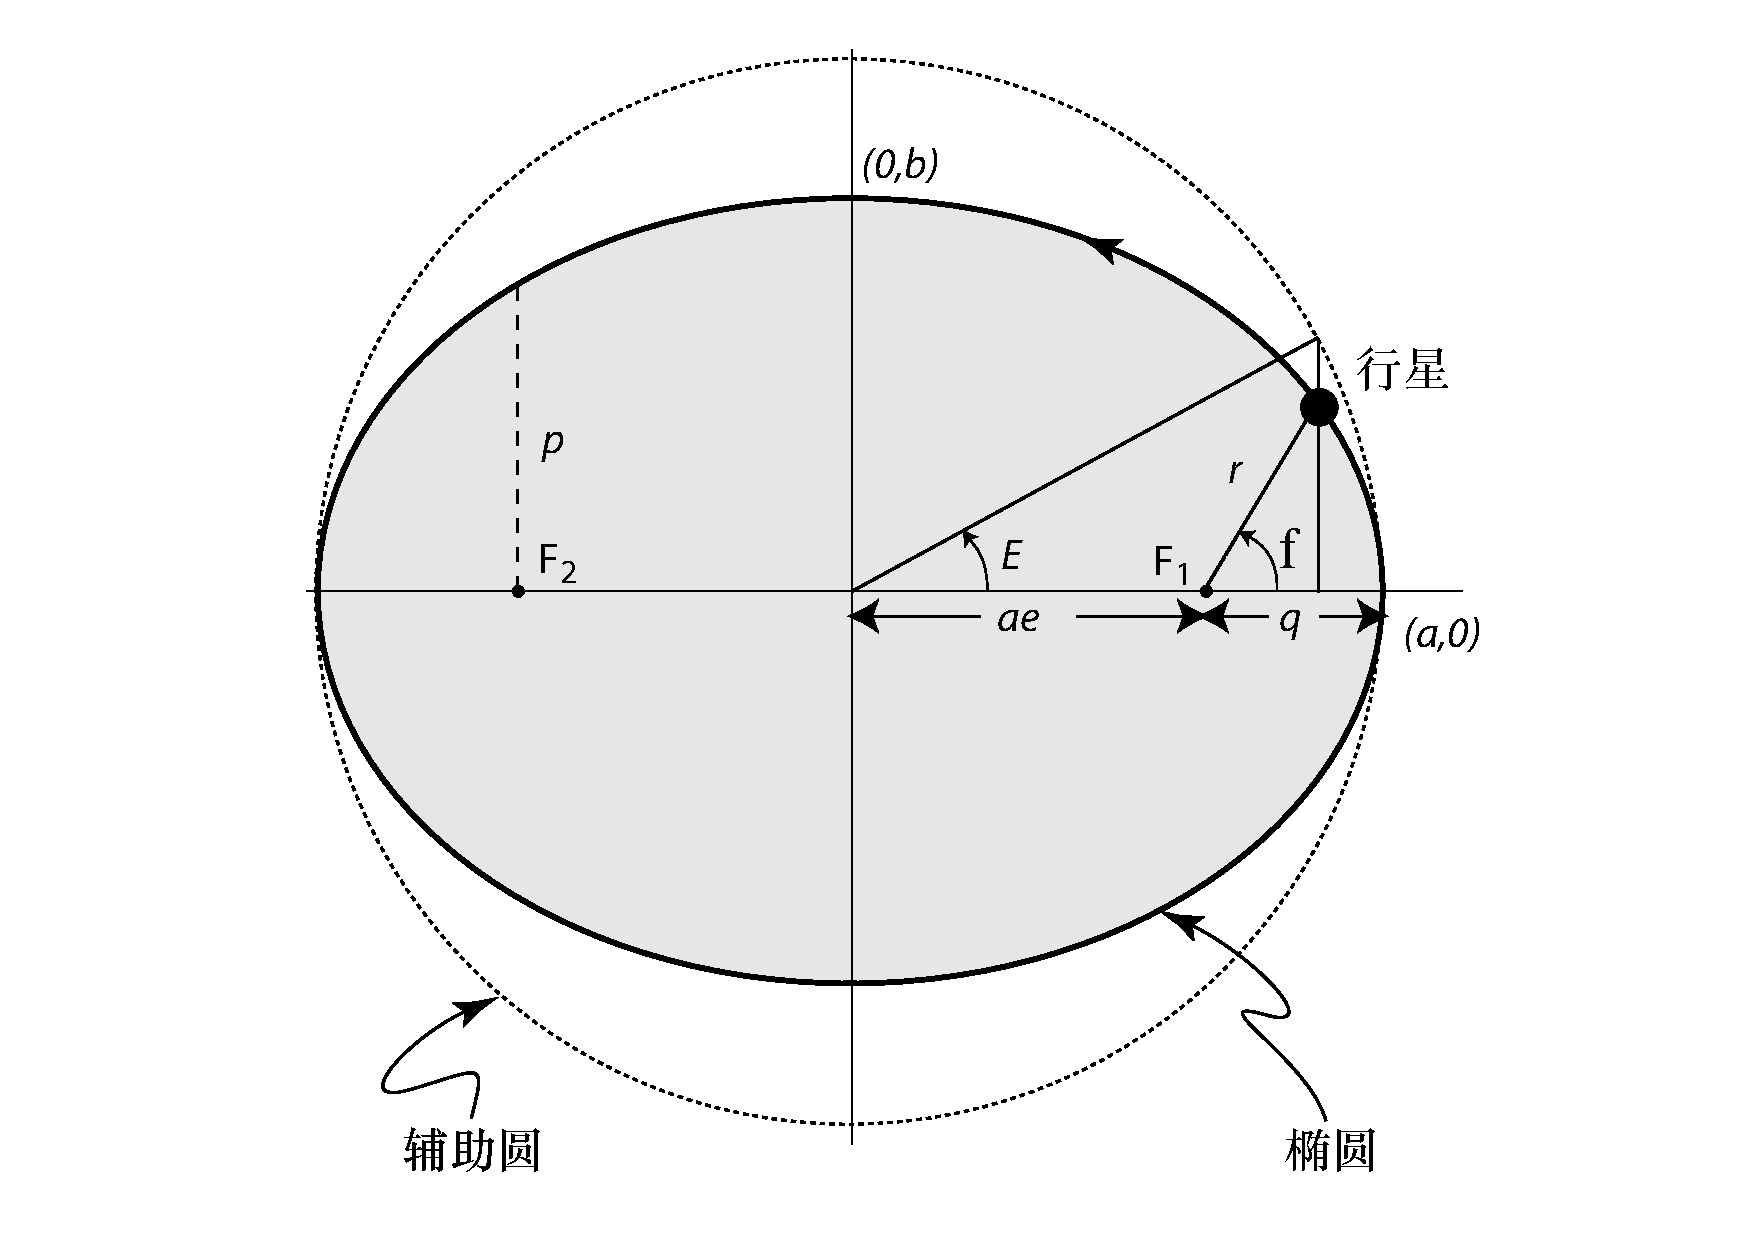
\includegraphics[width=0.95\textwidth]{figures/appendix/f1_ellipse.pdf}
\caption{二体在轨道平面内的椭圆运动示意图,图片来源 Perryman。}
\label{fig:ellipse}
\end{figure}

在次方反比的中心引力作用下,二体的运动轨迹为封闭的圆锥曲线\cite{Newton1687}。
图\ref{fig:ellipse} 和 \ref{fig:3dorbit} 展示的是椭圆二体运动示意图,其中 $a,\,e,\,i,\,\omega,\,\Omega,\,f$ 
被称作描述椭圆二体运动的六个轨道常数,文内符号几乎均沿袭自书本\citen{MurrayDermott1999ssd}。
在中心天体坐标系中,行星距离主星的标量距离 $r$ 可表示为:
\begin{equation} \label{radialdistance}
r = \frac{a(1-e^2)}{1+e\cos f}
\end{equation} %\myequation{二体运动的径向距离与轨道根素的关系}

\begin{figure}[t]
\centering
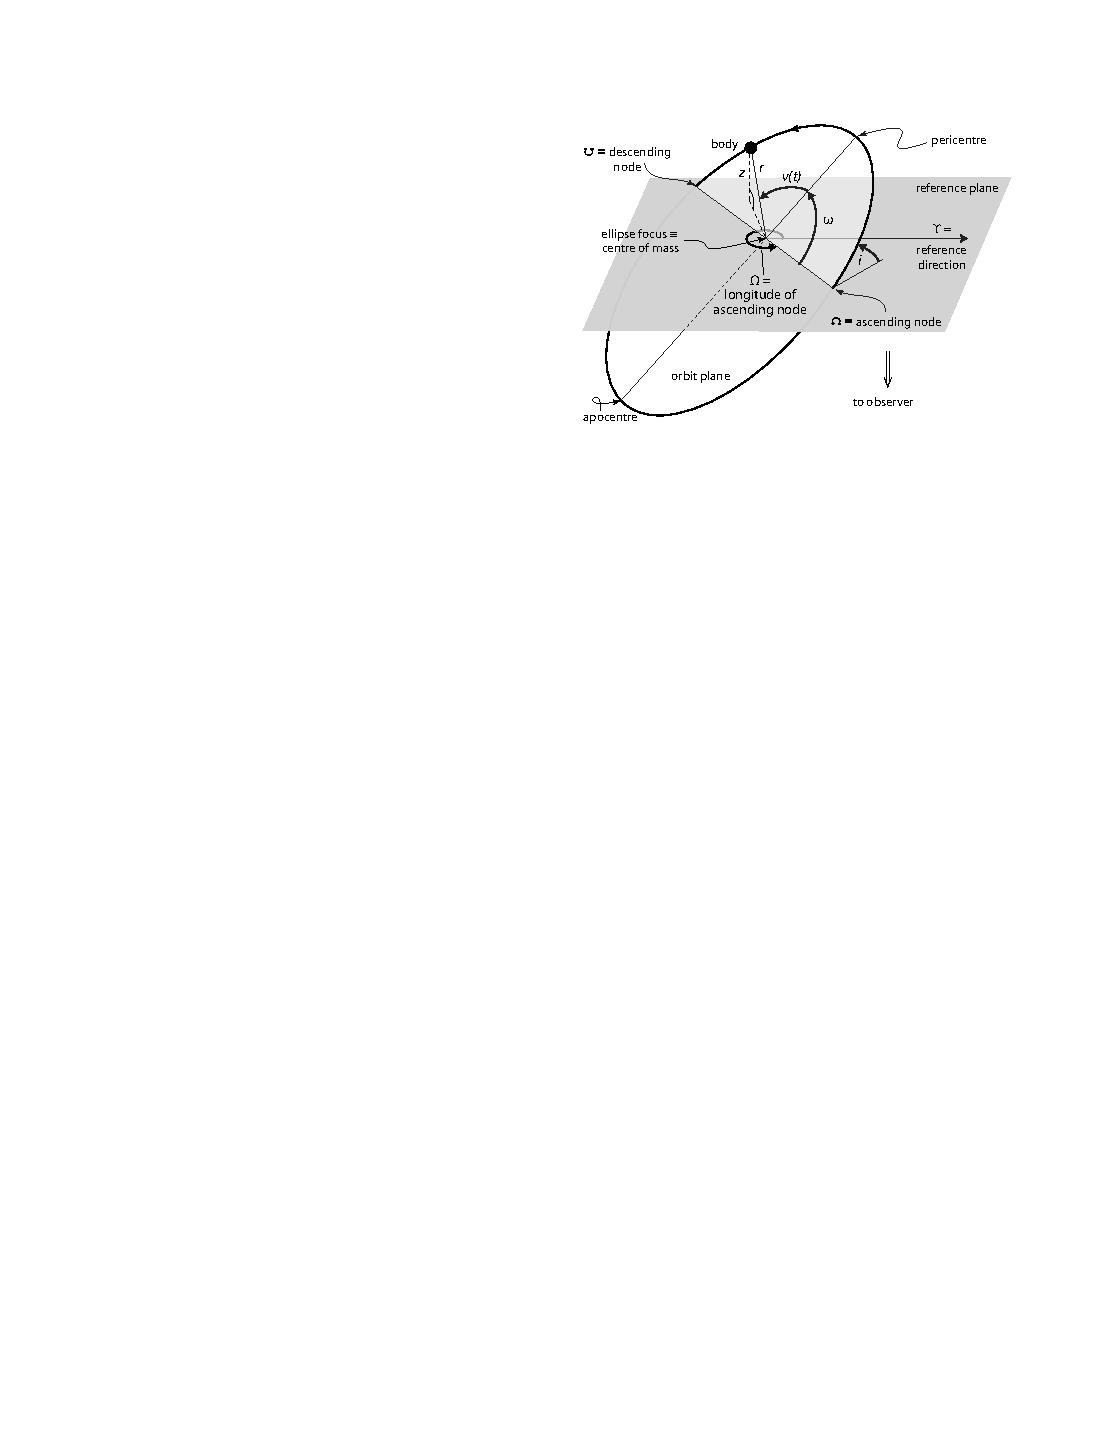
\includegraphics[width=0.95\textwidth]{figures/appendix/f2_3dorbit.pdf}
\caption{椭圆二体运动轨道在三维空间内的示意图,图内标识分别为轨道根数与参考系。图片来源 Perryman。}
\label{fig:3dorbit}
\end{figure}




%%%%%%%%%%%%%%%%%%%%%%%%%%%%%%%%%%%%%%%%%%%%%%%%%%%%%%%%%%%%%%%%%%%%%%%%%%%%%%%
% 书籍附件
\backmatter
%%%%%%%%%%%%%%%%%%%%%%%%%%%%%%%%%%%%%%%%%%%%%%%%%%%%%%%%%%%%%%%%%%%%%%%%%%%%%%%
% 作者简历与科研成果页,应放在backmatter之后
%%%%%%%%%%%%%%%%%%%%%%%%%%%%%%%%%%%%%%%%%%%%%%%%%%%%%%%%%%%%%%%%%%%%%%%%%%%%%%%
%%  
%% 文档类 NJU-Thesis 用户手册
%%
%% 作者:胡海星,starfish (at) gmail (dot) com
%% 项目主页: https://github.com/Haixing-Hu/nju-thesis
%%
%% This file may be distributed and/or modified under the conditions of the
%% LaTeX Project Public License, either version 1.2 of this license or (at your
%% option) any later version. The latest version of this license is in:
%%
%% http://www.latex-project.org/lppl.txt
%%
%% and version 1.2 or later is part of all distributions of LaTeX version
%% 1999/12/01 or later.
%%
%%%%%%%%%%%%%%%%%%%%%%%%%%%%%%%%%%%%%%%%%%%%%%%%%%%%%%%%%%%%%%%%%%%%%%%%%%%%%%%

\begin{resume}

\end{resume}
%%%%%%%%%%%%%%%%%%%%%%%%%%%%%%%%%%%%%%%%%%%%%%%%%%%%%%%%%%%%%%%%%%%%%%%%%%%%%%%
% 生成《学位论文出版授权书》页面,应放在最后一页
\makelicense
%%%%%%%%%%%%%%%%%%%%%%%%%%%%%%%%%%%%%%%%%%%%%%%%%%%%%%%%%%%%%%%%%%%%%%%%%%%%%%%
\end{document}
